% Options for packages loaded elsewhere
\PassOptionsToPackage{unicode}{hyperref}
\PassOptionsToPackage{hyphens}{url}
%
\documentclass[
  ignorenonframetext,
]{beamer}
\usepackage{pgfpages}
\setbeamertemplate{caption}[numbered]
\setbeamertemplate{caption label separator}{: }
\setbeamercolor{caption name}{fg=normal text.fg}
\beamertemplatenavigationsymbolsempty
% Prevent slide breaks in the middle of a paragraph
\widowpenalties 1 10000
\raggedbottom
\setbeamertemplate{part page}{
  \centering
  \begin{beamercolorbox}[sep=16pt,center]{part title}
    \usebeamerfont{part title}\insertpart\par
  \end{beamercolorbox}
}
\setbeamertemplate{section page}{
  \centering
  \begin{beamercolorbox}[sep=12pt,center]{part title}
    \usebeamerfont{section title}\insertsection\par
  \end{beamercolorbox}
}
\setbeamertemplate{subsection page}{
  \centering
  \begin{beamercolorbox}[sep=8pt,center]{part title}
    \usebeamerfont{subsection title}\insertsubsection\par
  \end{beamercolorbox}
}
\AtBeginPart{
  \frame{\partpage}
}
\AtBeginSection{
  \ifbibliography
  \else
    \frame{\sectionpage}
  \fi
}
\AtBeginSubsection{
  \frame{\subsectionpage}
}
\usepackage{lmodern}
\usepackage{amsmath}
\usepackage{ifxetex,ifluatex}
\ifnum 0\ifxetex 1\fi\ifluatex 1\fi=0 % if pdftex
  \usepackage[T1]{fontenc}
  \usepackage[utf8]{inputenc}
  \usepackage{textcomp} % provide euro and other symbols
  \usepackage{amssymb}
\else % if luatex or xetex
  \usepackage{unicode-math}
  \defaultfontfeatures{Scale=MatchLowercase}
  \defaultfontfeatures[\rmfamily]{Ligatures=TeX,Scale=1}
\fi
% Use upquote if available, for straight quotes in verbatim environments
\IfFileExists{upquote.sty}{\usepackage{upquote}}{}
\IfFileExists{microtype.sty}{% use microtype if available
  \usepackage[]{microtype}
  \UseMicrotypeSet[protrusion]{basicmath} % disable protrusion for tt fonts
}{}
\makeatletter
\@ifundefined{KOMAClassName}{% if non-KOMA class
  \IfFileExists{parskip.sty}{%
    \usepackage{parskip}
  }{% else
    \setlength{\parindent}{0pt}
    \setlength{\parskip}{6pt plus 2pt minus 1pt}}
}{% if KOMA class
  \KOMAoptions{parskip=half}}
\makeatother
\usepackage{xcolor}
\IfFileExists{xurl.sty}{\usepackage{xurl}}{} % add URL line breaks if available
\IfFileExists{bookmark.sty}{\usepackage{bookmark}}{\usepackage{hyperref}}
\hypersetup{
  pdftitle={Generalised Linear Models},
  pdfauthor={Joseph Bulbulia, Psychology, Victoria University},
  hidelinks,
  pdfcreator={LaTeX via pandoc}}
\urlstyle{same} % disable monospaced font for URLs
\newif\ifbibliography
\usepackage{color}
\usepackage{fancyvrb}
\newcommand{\VerbBar}{|}
\newcommand{\VERB}{\Verb[commandchars=\\\{\}]}
\DefineVerbatimEnvironment{Highlighting}{Verbatim}{commandchars=\\\{\}}
% Add ',fontsize=\small' for more characters per line
\usepackage{framed}
\definecolor{shadecolor}{RGB}{248,248,248}
\newenvironment{Shaded}{\begin{snugshade}}{\end{snugshade}}
\newcommand{\AlertTok}[1]{\textcolor[rgb]{0.94,0.16,0.16}{#1}}
\newcommand{\AnnotationTok}[1]{\textcolor[rgb]{0.56,0.35,0.01}{\textbf{\textit{#1}}}}
\newcommand{\AttributeTok}[1]{\textcolor[rgb]{0.77,0.63,0.00}{#1}}
\newcommand{\BaseNTok}[1]{\textcolor[rgb]{0.00,0.00,0.81}{#1}}
\newcommand{\BuiltInTok}[1]{#1}
\newcommand{\CharTok}[1]{\textcolor[rgb]{0.31,0.60,0.02}{#1}}
\newcommand{\CommentTok}[1]{\textcolor[rgb]{0.56,0.35,0.01}{\textit{#1}}}
\newcommand{\CommentVarTok}[1]{\textcolor[rgb]{0.56,0.35,0.01}{\textbf{\textit{#1}}}}
\newcommand{\ConstantTok}[1]{\textcolor[rgb]{0.00,0.00,0.00}{#1}}
\newcommand{\ControlFlowTok}[1]{\textcolor[rgb]{0.13,0.29,0.53}{\textbf{#1}}}
\newcommand{\DataTypeTok}[1]{\textcolor[rgb]{0.13,0.29,0.53}{#1}}
\newcommand{\DecValTok}[1]{\textcolor[rgb]{0.00,0.00,0.81}{#1}}
\newcommand{\DocumentationTok}[1]{\textcolor[rgb]{0.56,0.35,0.01}{\textbf{\textit{#1}}}}
\newcommand{\ErrorTok}[1]{\textcolor[rgb]{0.64,0.00,0.00}{\textbf{#1}}}
\newcommand{\ExtensionTok}[1]{#1}
\newcommand{\FloatTok}[1]{\textcolor[rgb]{0.00,0.00,0.81}{#1}}
\newcommand{\FunctionTok}[1]{\textcolor[rgb]{0.00,0.00,0.00}{#1}}
\newcommand{\ImportTok}[1]{#1}
\newcommand{\InformationTok}[1]{\textcolor[rgb]{0.56,0.35,0.01}{\textbf{\textit{#1}}}}
\newcommand{\KeywordTok}[1]{\textcolor[rgb]{0.13,0.29,0.53}{\textbf{#1}}}
\newcommand{\NormalTok}[1]{#1}
\newcommand{\OperatorTok}[1]{\textcolor[rgb]{0.81,0.36,0.00}{\textbf{#1}}}
\newcommand{\OtherTok}[1]{\textcolor[rgb]{0.56,0.35,0.01}{#1}}
\newcommand{\PreprocessorTok}[1]{\textcolor[rgb]{0.56,0.35,0.01}{\textit{#1}}}
\newcommand{\RegionMarkerTok}[1]{#1}
\newcommand{\SpecialCharTok}[1]{\textcolor[rgb]{0.00,0.00,0.00}{#1}}
\newcommand{\SpecialStringTok}[1]{\textcolor[rgb]{0.31,0.60,0.02}{#1}}
\newcommand{\StringTok}[1]{\textcolor[rgb]{0.31,0.60,0.02}{#1}}
\newcommand{\VariableTok}[1]{\textcolor[rgb]{0.00,0.00,0.00}{#1}}
\newcommand{\VerbatimStringTok}[1]{\textcolor[rgb]{0.31,0.60,0.02}{#1}}
\newcommand{\WarningTok}[1]{\textcolor[rgb]{0.56,0.35,0.01}{\textbf{\textit{#1}}}}
\usepackage{graphicx}
\makeatletter
\def\maxwidth{\ifdim\Gin@nat@width>\linewidth\linewidth\else\Gin@nat@width\fi}
\def\maxheight{\ifdim\Gin@nat@height>\textheight\textheight\else\Gin@nat@height\fi}
\makeatother
% Scale images if necessary, so that they will not overflow the page
% margins by default, and it is still possible to overwrite the defaults
% using explicit options in \includegraphics[width, height, ...]{}
\setkeys{Gin}{width=\maxwidth,height=\maxheight,keepaspectratio}
% Set default figure placement to htbp
\makeatletter
\def\fps@figure{htbp}
\makeatother
\setlength{\emergencystretch}{3em} % prevent overfull lines
\providecommand{\tightlist}{%
  \setlength{\itemsep}{0pt}\setlength{\parskip}{0pt}}
\setcounter{secnumdepth}{-\maxdimen} % remove section numbering
\ifluatex
  \usepackage{selnolig}  % disable illegal ligatures
\fi
\newlength{\cslhangindent}
\setlength{\cslhangindent}{1.5em}
\newlength{\csllabelwidth}
\setlength{\csllabelwidth}{3em}
\newenvironment{CSLReferences}[2] % #1 hanging-ident, #2 entry spacing
 {% don't indent paragraphs
  \setlength{\parindent}{0pt}
  % turn on hanging indent if param 1 is 1
  \ifodd #1 \everypar{\setlength{\hangindent}{\cslhangindent}}\ignorespaces\fi
  % set entry spacing
  \ifnum #2 > 0
  \setlength{\parskip}{#2\baselineskip}
  \fi
 }%
 {}
\usepackage{calc}
\newcommand{\CSLBlock}[1]{#1\hfill\break}
\newcommand{\CSLLeftMargin}[1]{\parbox[t]{\csllabelwidth}{#1}}
\newcommand{\CSLRightInline}[1]{\parbox[t]{\linewidth - \csllabelwidth}{#1}\break}
\newcommand{\CSLIndent}[1]{\hspace{\cslhangindent}#1}

\title{Generalised Linear Models}
\author{Joseph Bulbulia, Psychology, Victoria University}
\date{2020-APRIL-27}

\begin{document}
\frame{\titlepage}

\begin{frame}[fragile]
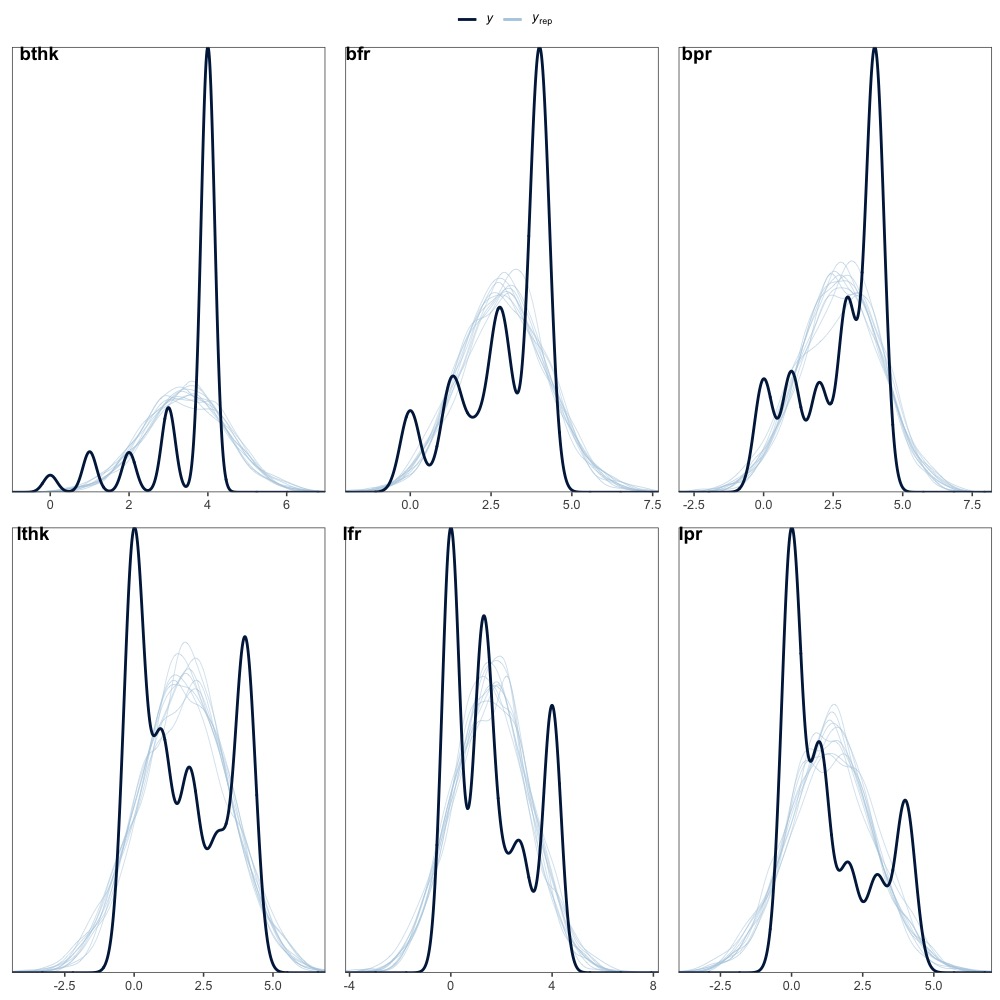
\includegraphics[width=13.89in]{op}

\begin{block}{Generalised linear models}
\protect\hypertarget{generalised-linear-models}{}
\end{block}

\begin{block}{Objectives}
\protect\hypertarget{objectives}{}
\begin{enumerate}[<+->]
\tightlist
\item
  logistic regression models, which apply to \emph{binary} responses;
\item
  Poisson regression models, which apply to \emph{rates};
\item
  over-dispersed poisson models.
\item
  Zero-inflated poisson models, in which rates data contain an
  over-abundance of zeros.
\end{enumerate}
\end{block}

\begin{block}{Introduction}
\protect\hypertarget{introduction}{}
Our regression workflow is built on two imperatives:

\begin{enumerate}[<+->]
[(1)]
\tightlist
\item
  to clarify our assumptions;
\item
  to clarify our decisions.
\end{enumerate}
\end{block}

\begin{block}{Linear regression: Fit a line}
\protect\hypertarget{linear-regression-fit-a-line}{}
\[
y_i \sim Normal ( \mu_i, \sigma)\\
\sigma \sim Exponentional (1) \\
\mu_i \sim \alpha + \beta x_i \\
\boldsymbol{\eta} =  \boldsymbol{\alpha} + \boldsymbol{X}\boldsymbol{\beta}\\
\]
\end{block}

\begin{block}{Generalised linear model implies a `link' function}
\protect\hypertarget{generalised-linear-model-implies-a-link-function}{}
\(g(\cdot)\) = link function \$h(\cdot) = g\^{}-1(\cdot) \$ = inverse
link function

Where \((\cdot)\) is the linear predictor: \(\mathboldsymbol{\eta}\)
\end{block}

\begin{block}{Logistic regression}
\protect\hypertarget{logistic-regression}{}
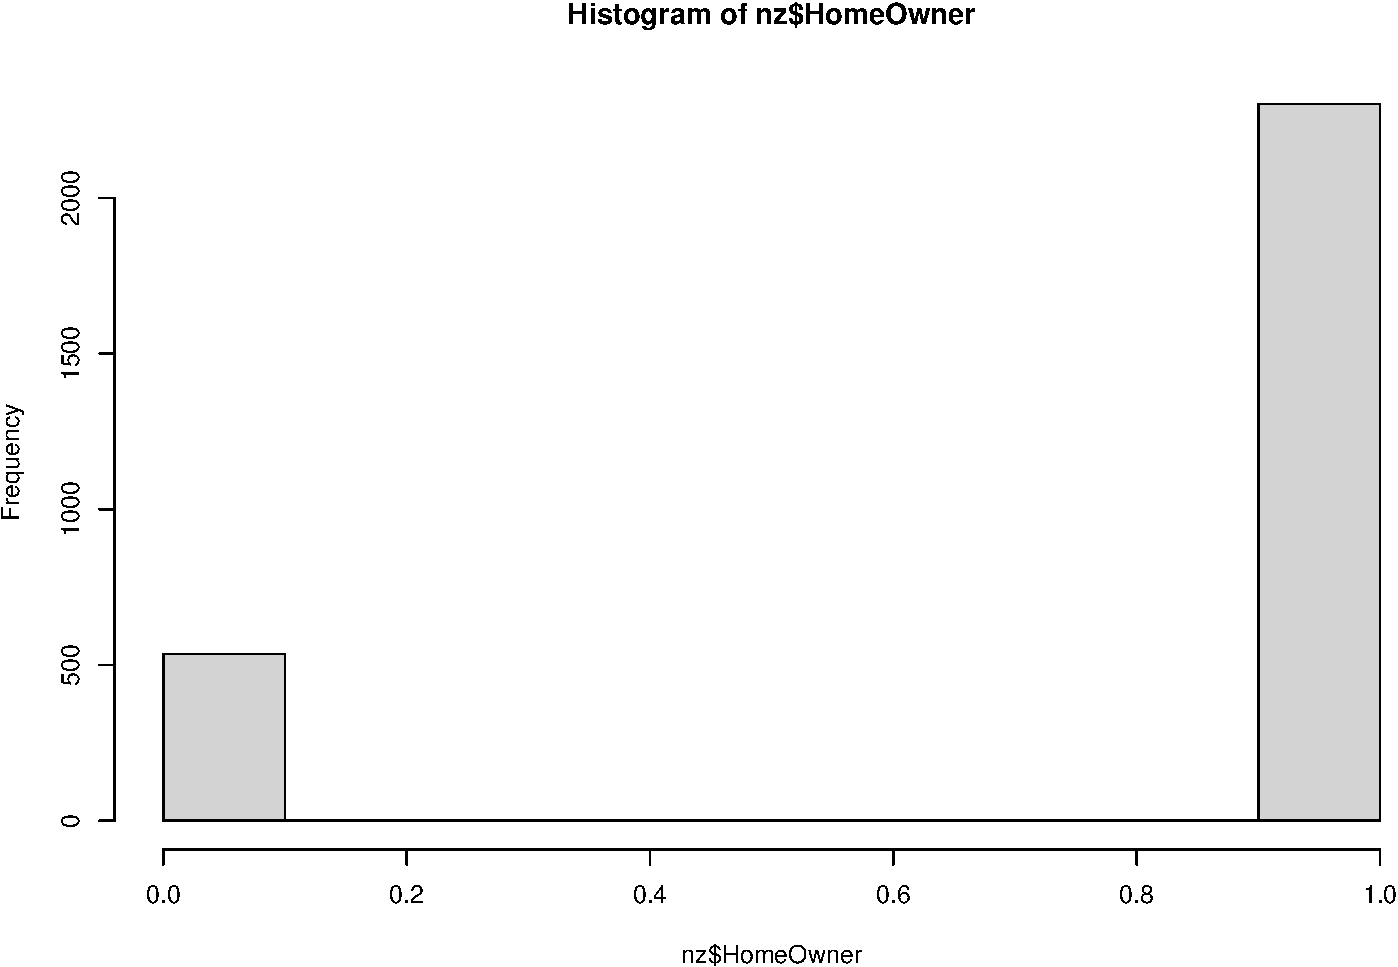
\includegraphics{slides_files/figure-beamer/unnamed-chunk-1-1.pdf}
\end{block}

\begin{block}{Link function for logistic regression}
\protect\hypertarget{link-function-for-logistic-regression}{}
The model requires a binomial link function:

\[Home_i \sim Binomial (Ownership_i, Pr)\]
\end{block}

\begin{block}{The binomial link function does two things}
\protect\hypertarget{the-binomial-link-function-does-two-things}{}
\begin{itemize}[<+->]
\tightlist
\item
  first, it maps the range \((0, 1)\) to \(-(\infty, -\infty)\).
\item
  second, it maps these values back to the unit range (see: Gelman,
  Hill, and Vehtari (2020) )
\end{itemize}
\end{block}

\begin{block}{The logistic function satisfies the first task:}
\protect\hypertarget{the-logistic-function-satisfies-the-first-task}{}
\(logit(\cdot) = log_e\frac{p}{(1-p)}\)
\end{block}

\begin{block}{The inverse logit functionsatisfies the second task:}
\protect\hypertarget{the-inverse-logit-functionsatisfies-the-second-task}{}
\(logit^-1(\cdot) = log\frac{e^\cdot}{(1-e^\cdot)}\)
\end{block}

\begin{block}{We write this}
\protect\hypertarget{we-write-this}{}
\[
\Pr(y_i = 1) = p_i \\
logit(p_i) = \alpha + \beta x_i \\
\Pr(y_i = 1) = logit^{-1}(\alpha + \beta x_i)
\]
\end{block}

\begin{block}{Logistic regression model}
\protect\hypertarget{logistic-regression-model}{}
\end{block}

\begin{block}{Result}
\protect\hypertarget{result}{}
\begin{verbatim}
## Parameter   | Log-Odds |   SE |       95% CI |     z |      p
## -------------------------------------------------------------
## (Intercept) |     1.46 | 0.05 | [1.36, 1.55] | 30.38 | < .001
\end{verbatim}
\end{block}

\begin{block}{Equation form}
\protect\hypertarget{equation-form}{}
\[
\log\left[ \frac { \widehat{P( \operatorname{HomeOwner} = \operatorname{1} )} }{ 1 - \widehat{P( \operatorname{HomeOwner} = \operatorname{1} )} } \right] = 1.46
\]

\begin{block}{Intepretation using \texttt{plogis}}
\protect\hypertarget{intepretation-using-plogis}{}
\begin{verbatim}
## [1] 0.811068
\end{verbatim}
\end{block}
\end{block}
\end{frame}

\begin{frame}[fragile]{Logistic regression with a single co-variate.}
\protect\hypertarget{logistic-regression-with-a-single-co-variate.}{}
\begin{block}{Workflow: center and scale continuous predictors}
\protect\hypertarget{workflow-center-and-scale-continuous-predictors}{}
\end{block}

\begin{block}{Model syntax}
\protect\hypertarget{model-syntax}{}
\end{block}

\begin{block}{Results}
\protect\hypertarget{results}{}
\begin{verbatim}
## Parameter       | Log-Odds |   SE |       95% CI |     z |      p
## -----------------------------------------------------------------
## (Intercept)     |     1.58 | 0.05 | [1.48, 1.69] | 29.37 | < .001
## Household.INC_s |     0.72 | 0.08 | [0.57, 0.89] |  8.86 | < .001
\end{verbatim}

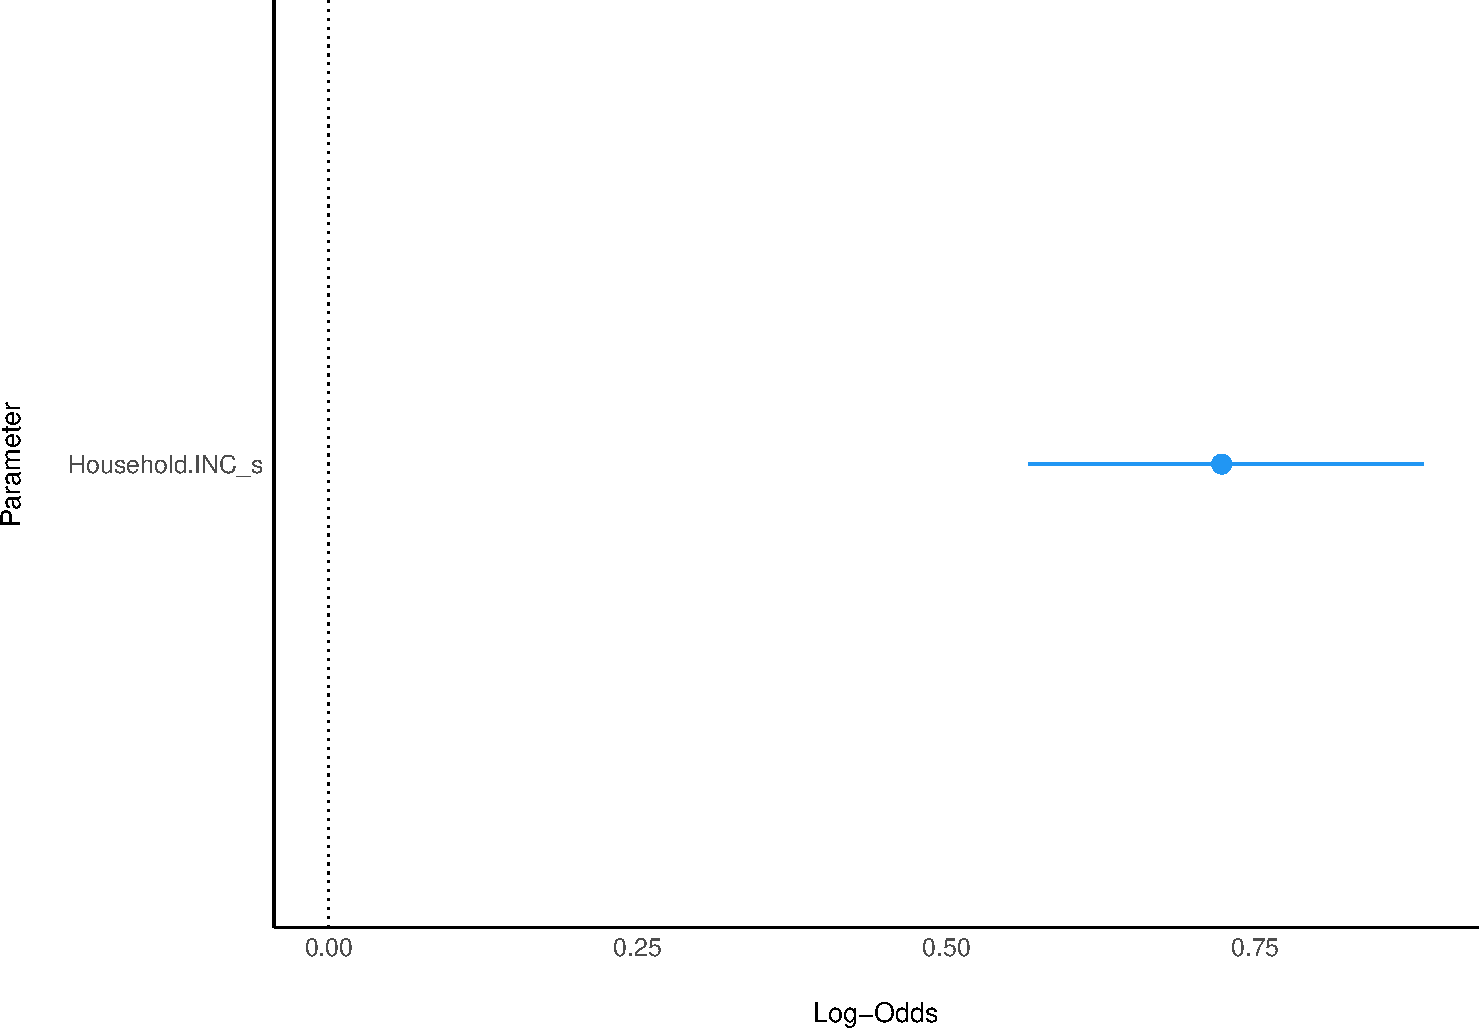
\includegraphics{slides_files/figure-beamer/unnamed-chunk-8-1.pdf}
\end{block}

\begin{block}{Equation form}
\protect\hypertarget{equation-form-1}{}
\[
\log\left[ \frac { \widehat{P( \operatorname{HomeOwner} = \operatorname{1} )} }{ 1 - \widehat{P( \operatorname{HomeOwner} = \operatorname{1} )} } \right] = 1.58 + 0.72(\operatorname{Household.INC\_s})
\]

\begin{block}{Interpretation not clear}
\protect\hypertarget{interpretation-not-clear}{}
\begin{verbatim}
## We fitted a logistic model (estimated using ML) to predict HomeOwner with Household.INC_s (formula: HomeOwner ~ Household.INC_s). The model's explanatory power is weak (Tjur's R2 = 0.04). The model's intercept, corresponding to Household.INC_s = 0, is at 1.58 (95% CI [1.48, 1.69], p < .001). Within this model:
## 
##   - The effect of Household.INC_s is significantly positive (beta = 0.72, 95% CI [0.57, 0.89], p < .001; Std. beta = 0.73, 95% CI [0.57, 0.89])
## 
## Standardized parameters were obtained by fitting the model on a standardized version of the dataset. 95% Confidence Intervals (CIs) and p-values were computed using
\end{verbatim}
\end{block}
\end{block}

\begin{block}{Graph your results!}
\protect\hypertarget{graph-your-results}{}
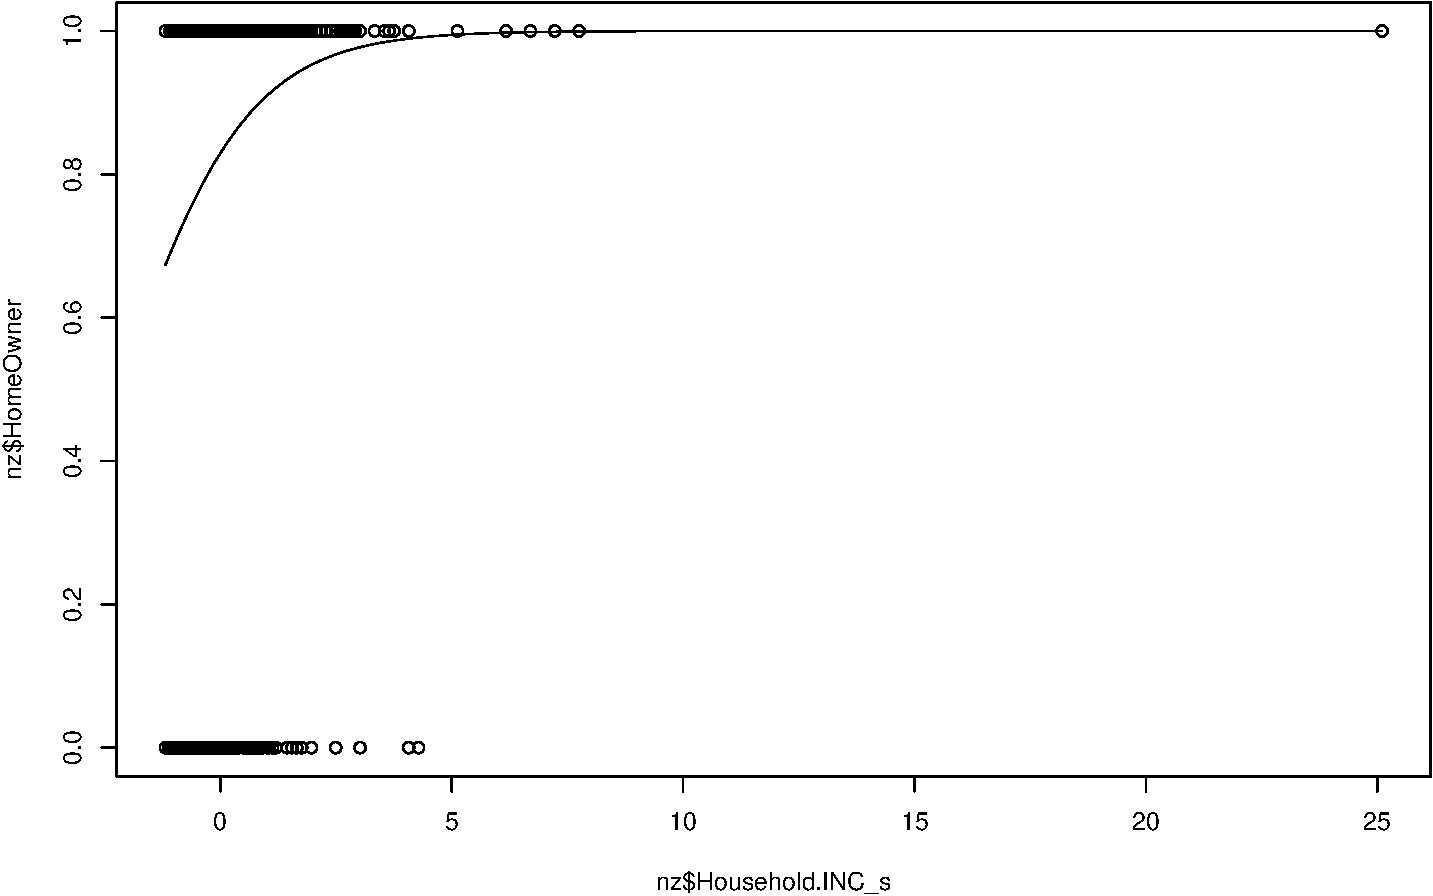
\includegraphics{slides_files/figure-beamer/unnamed-chunk-11-1.pdf}
\end{block}

\begin{block}{Alternative graph}
\protect\hypertarget{alternative-graph}{}
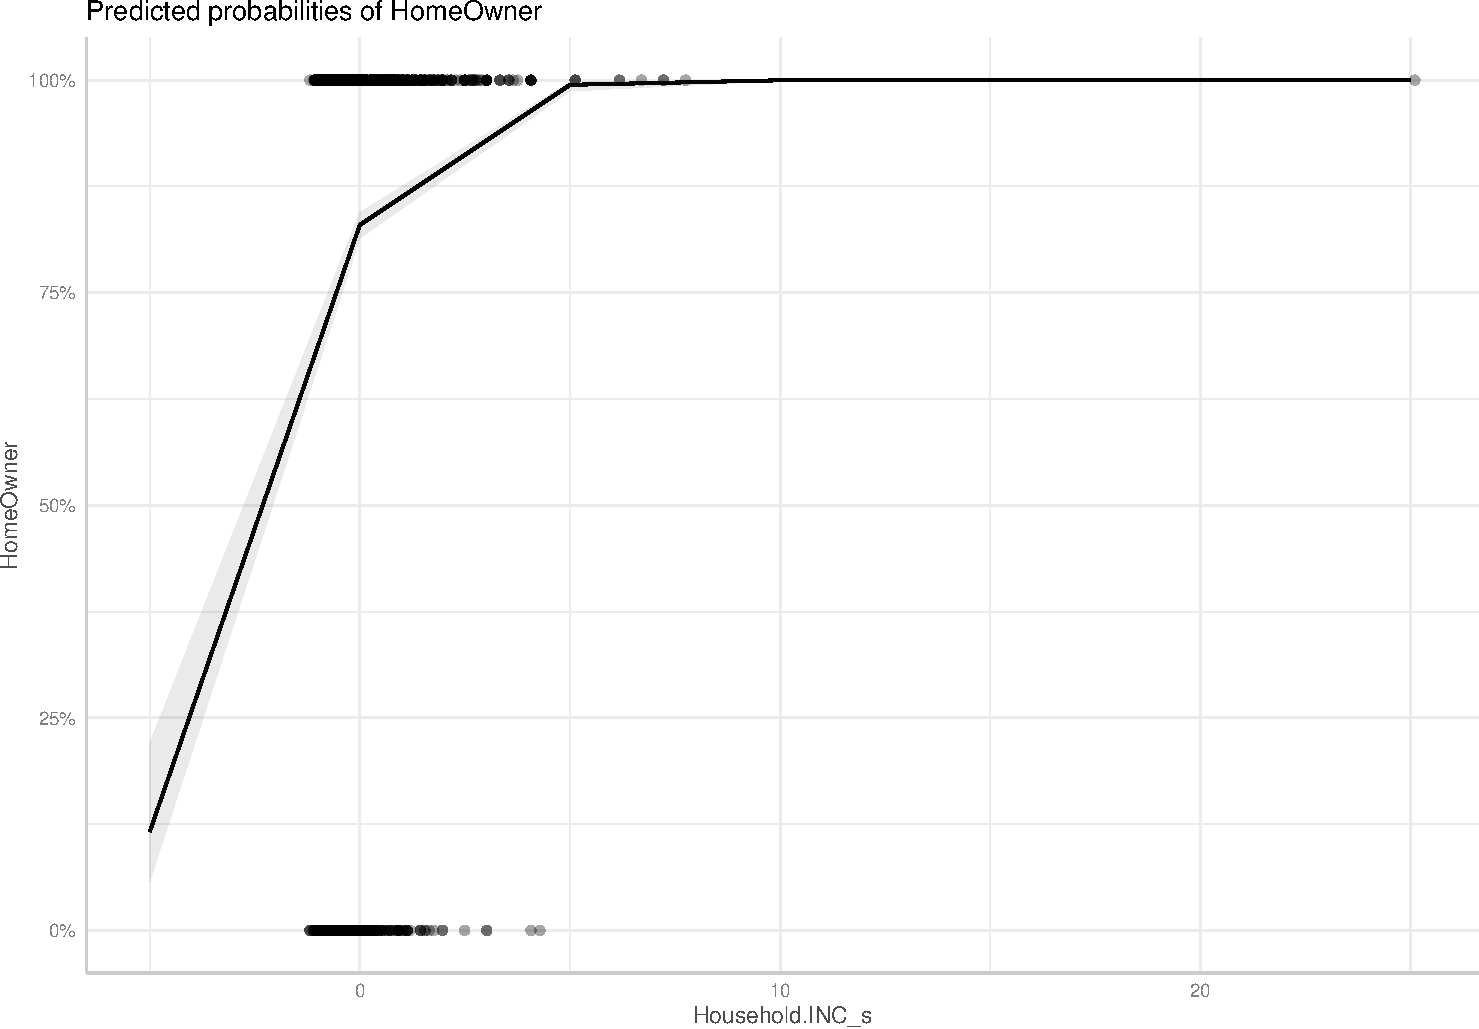
\includegraphics{slides_files/figure-beamer/unnamed-chunk-12-1.pdf}
\end{block}

\begin{block}{Spread of income}
\protect\hypertarget{spread-of-income}{}
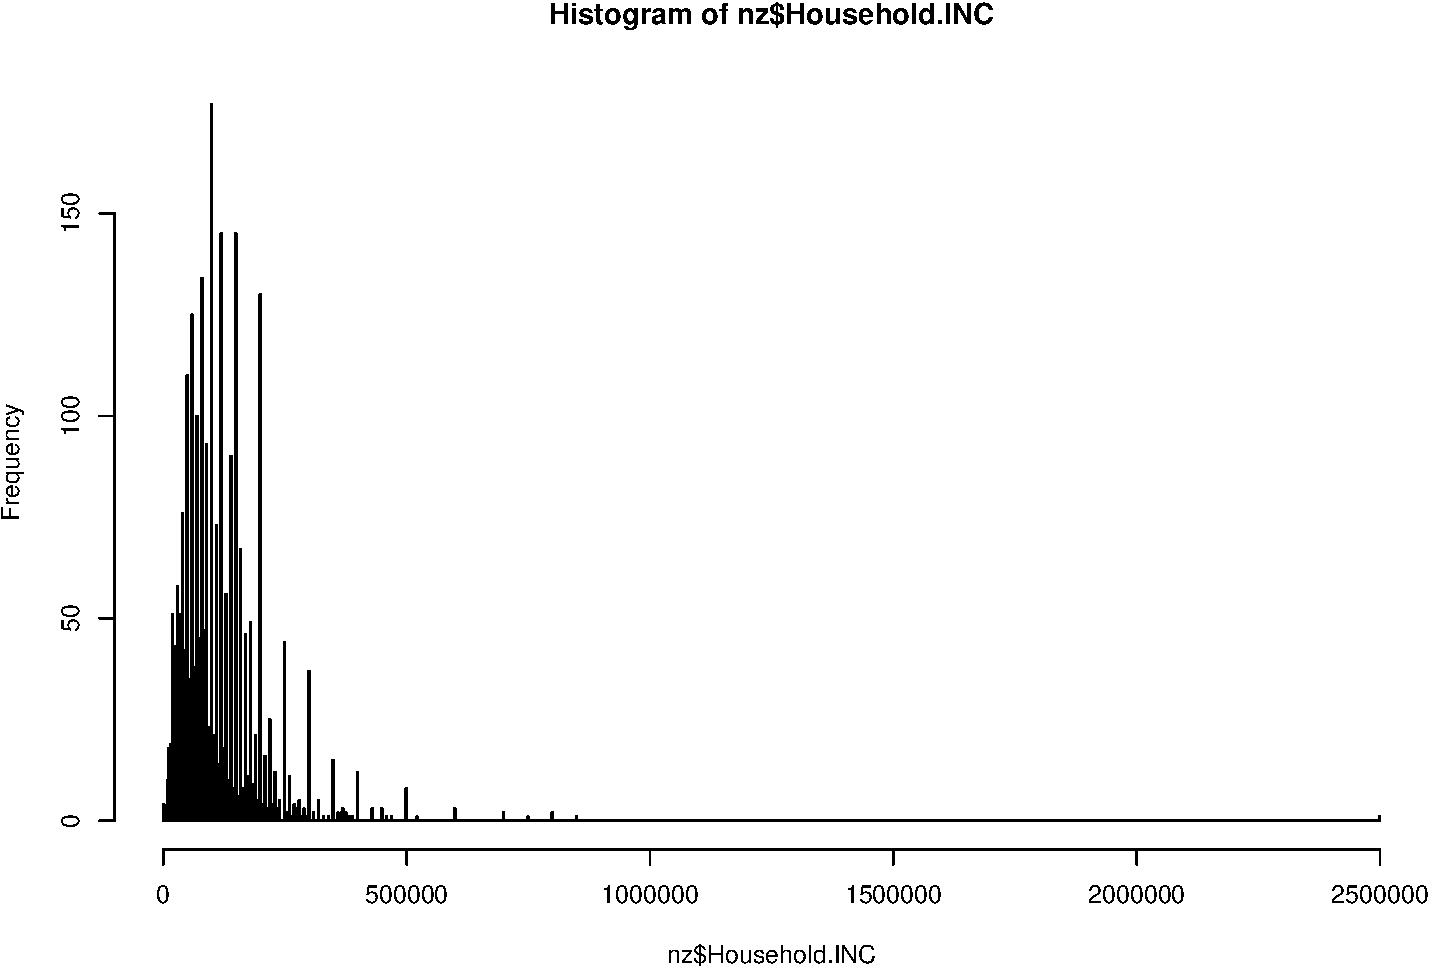
\includegraphics{slides_files/figure-beamer/unnamed-chunk-13-1.pdf}
\end{block}

\begin{block}{Range of income}
\protect\hypertarget{range-of-income}{}
The range of incomes is: 0, \ensuremath{2.5\times 10^{6}}.
\end{block}

\begin{block}{Sensitivity to outliers?}
\protect\hypertarget{sensitivity-to-outliers}{}
\begin{verbatim}
## [1] 0.979438
\end{verbatim}
\end{block}

\begin{block}{Alternative model}
\protect\hypertarget{alternative-model}{}
\begin{verbatim}
## Parameter       | Log-Odds |   SE |       95% CI |     z |      p
## -----------------------------------------------------------------
## (Intercept)     |     1.60 | 0.05 | [1.50, 1.71] | 29.21 | < .001
## Household.INC_s |     0.78 | 0.08 | [0.62, 0.95] |  9.27 | < .001
\end{verbatim}
\end{block}

\begin{block}{Range of predictors}
\protect\hypertarget{range-of-predictors}{}
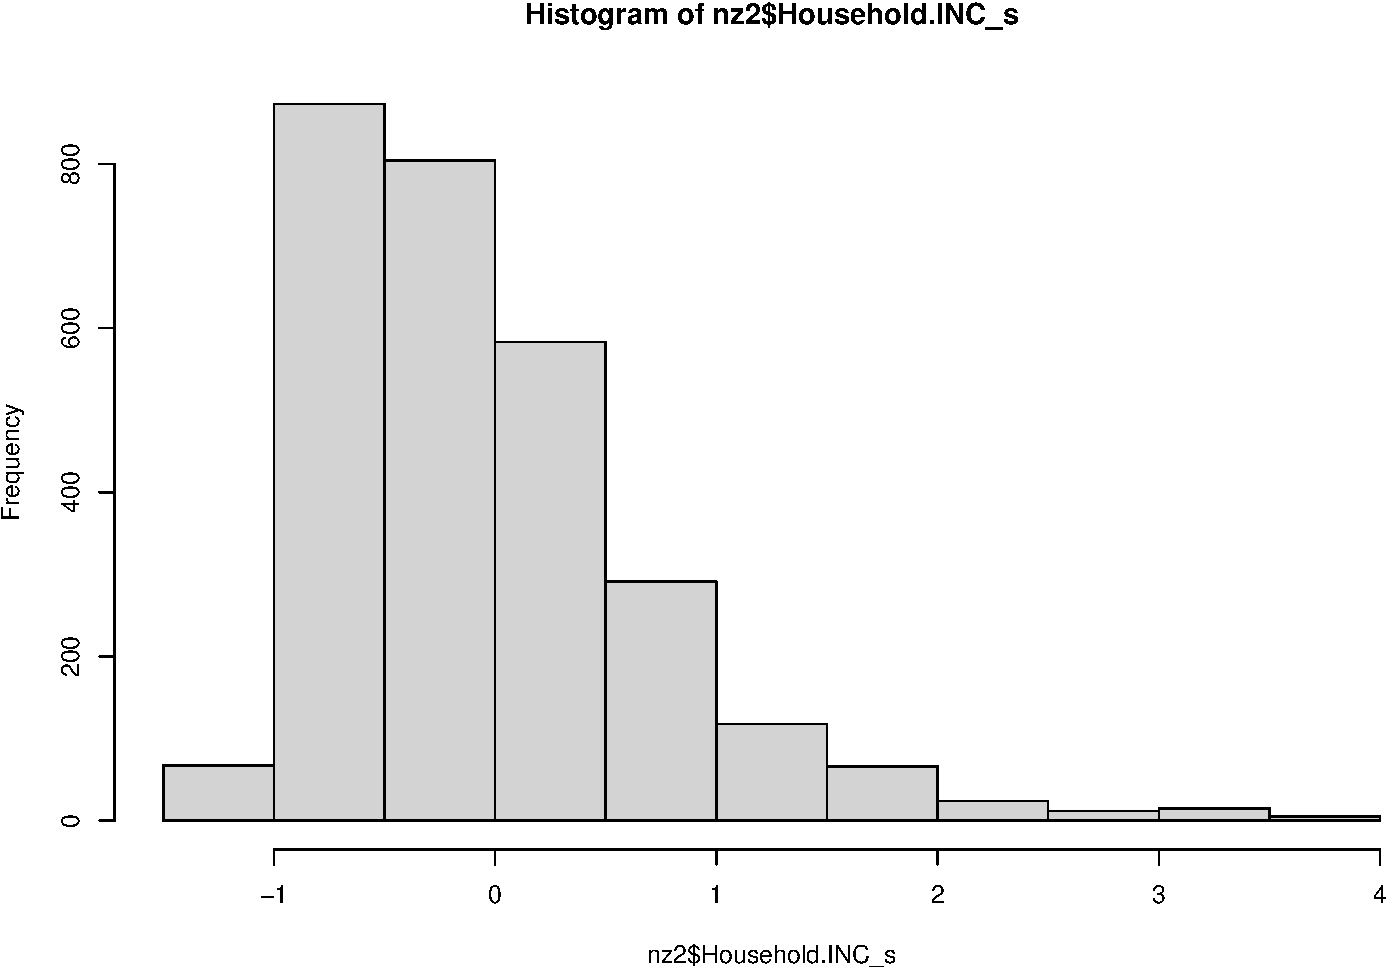
\includegraphics{slides_files/figure-beamer/unnamed-chunk-16-1.pdf}
\end{block}

\begin{block}{Model with extreme values removed}
\protect\hypertarget{model-with-extreme-values-removed}{}
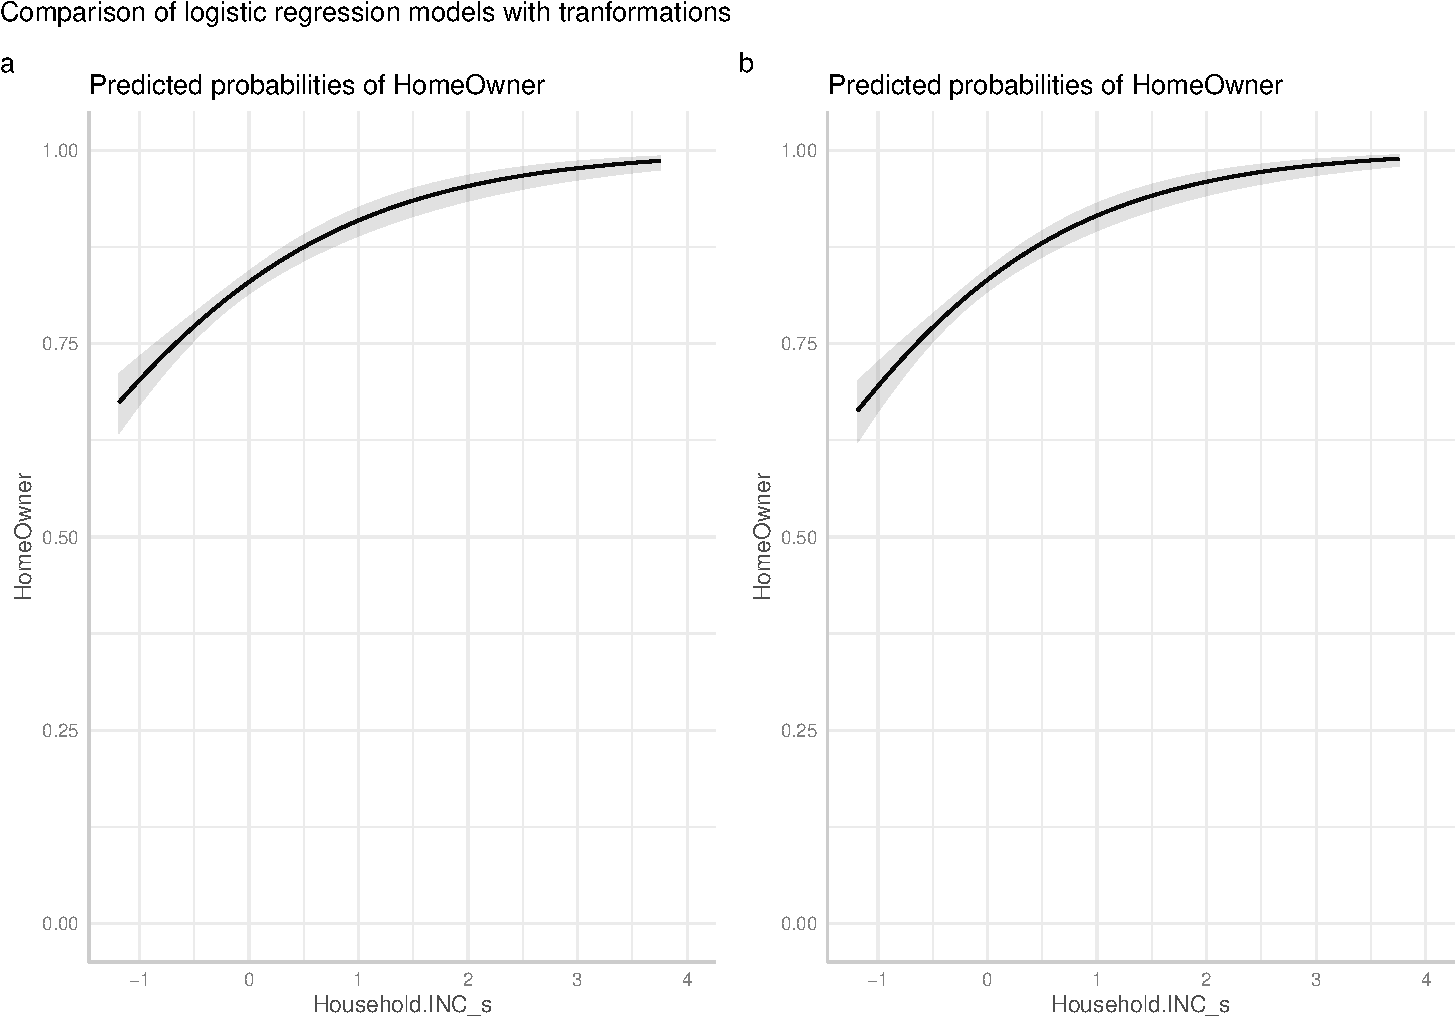
\includegraphics{slides_files/figure-beamer/unnamed-chunk-17-1.pdf}
\end{block}

\begin{block}{Aside: a trick}
\protect\hypertarget{aside-a-trick}{}
\texttt{scale\_x\_continuous(limits\ =\ c(-1.2,\ 4))}

This code allowed me to constrain both graphs to the same x-axis scale.
If I left this out the graphs would have looked like this:

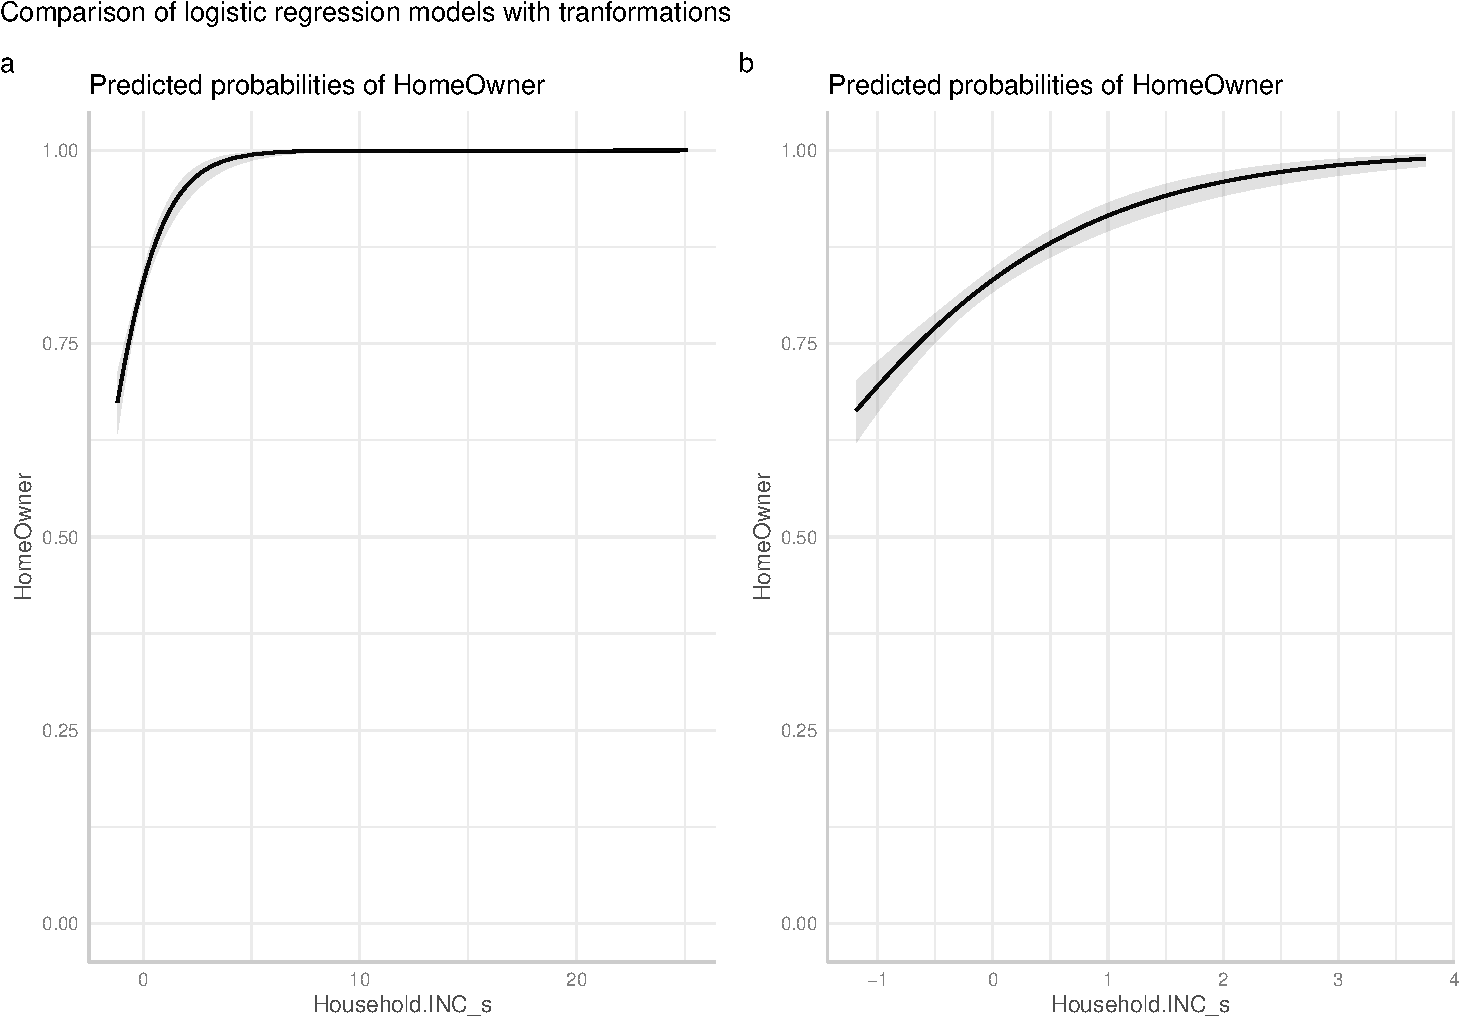
\includegraphics{slides_files/figure-beamer/unnamed-chunk-18-1.pdf}
\end{block}

\begin{block}{What if we used \texttt{lm}}
\protect\hypertarget{what-if-we-used-lm}{}
\begin{verbatim}
## Parameter       | Coefficient |       SE |       95% CI | t(2796) |      p
## --------------------------------------------------------------------------
## (Intercept)     |        0.81 | 7.27e-03 | [0.80, 0.83] |  111.88 | < .001
## Household.INC_s |        0.06 | 7.23e-03 | [0.04, 0.07] |    8.04 | < .001
\end{verbatim}

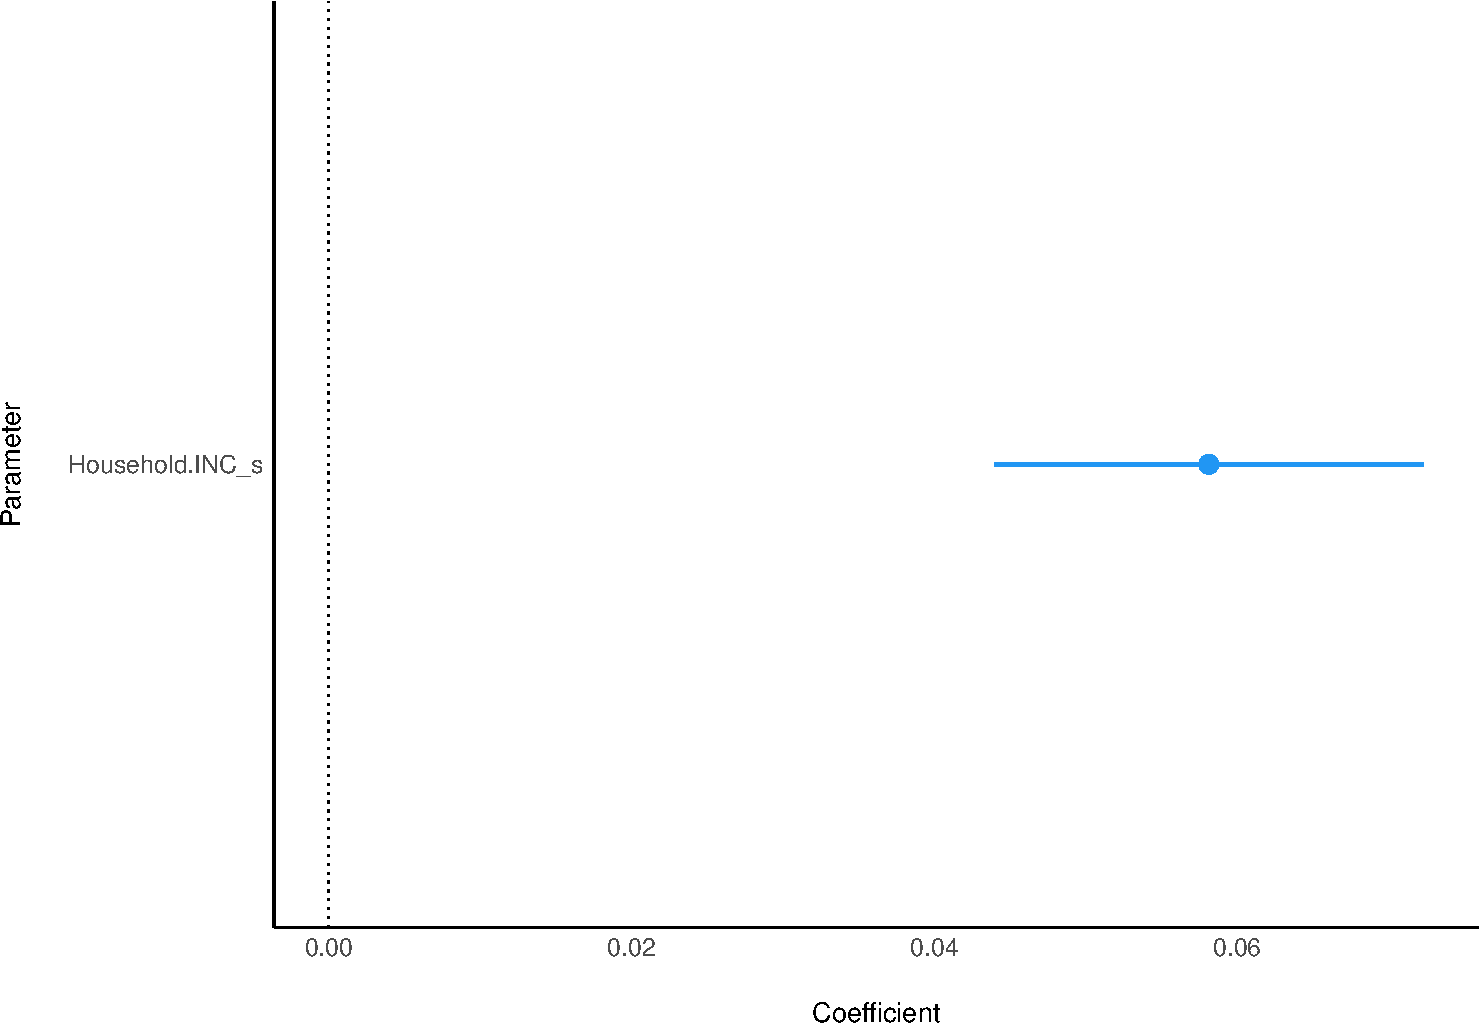
\includegraphics{slides_files/figure-beamer/unnamed-chunk-19-1.pdf}
\end{block}

\begin{block}{Compare graphs}
\protect\hypertarget{compare-graphs}{}
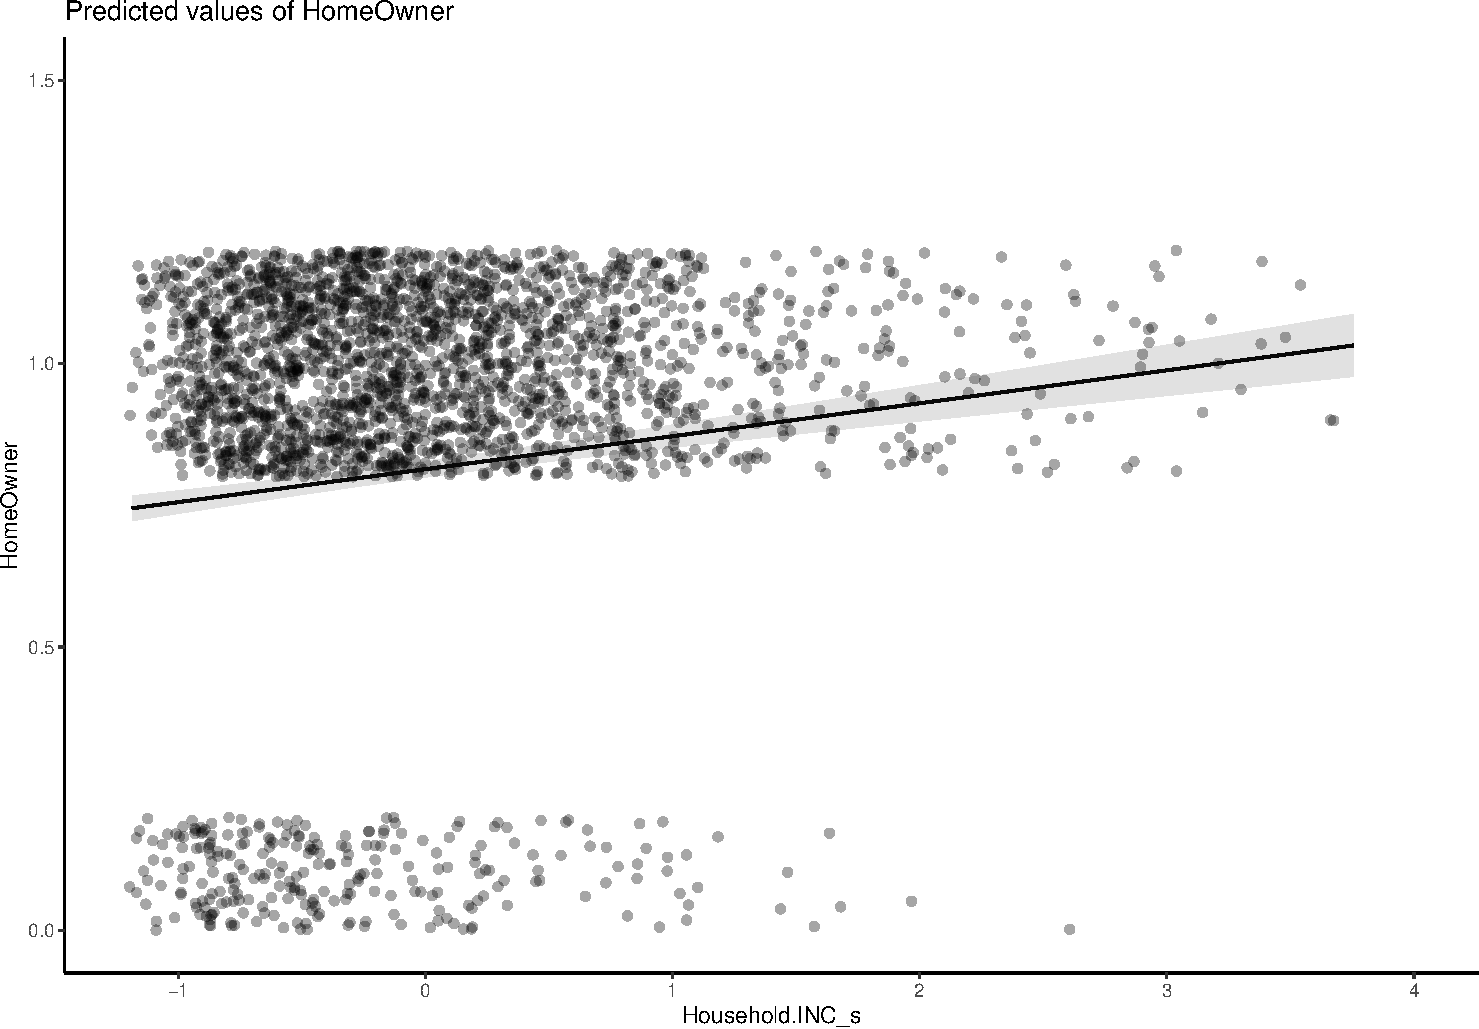
\includegraphics{slides_files/figure-beamer/unnamed-chunk-20-1.pdf}
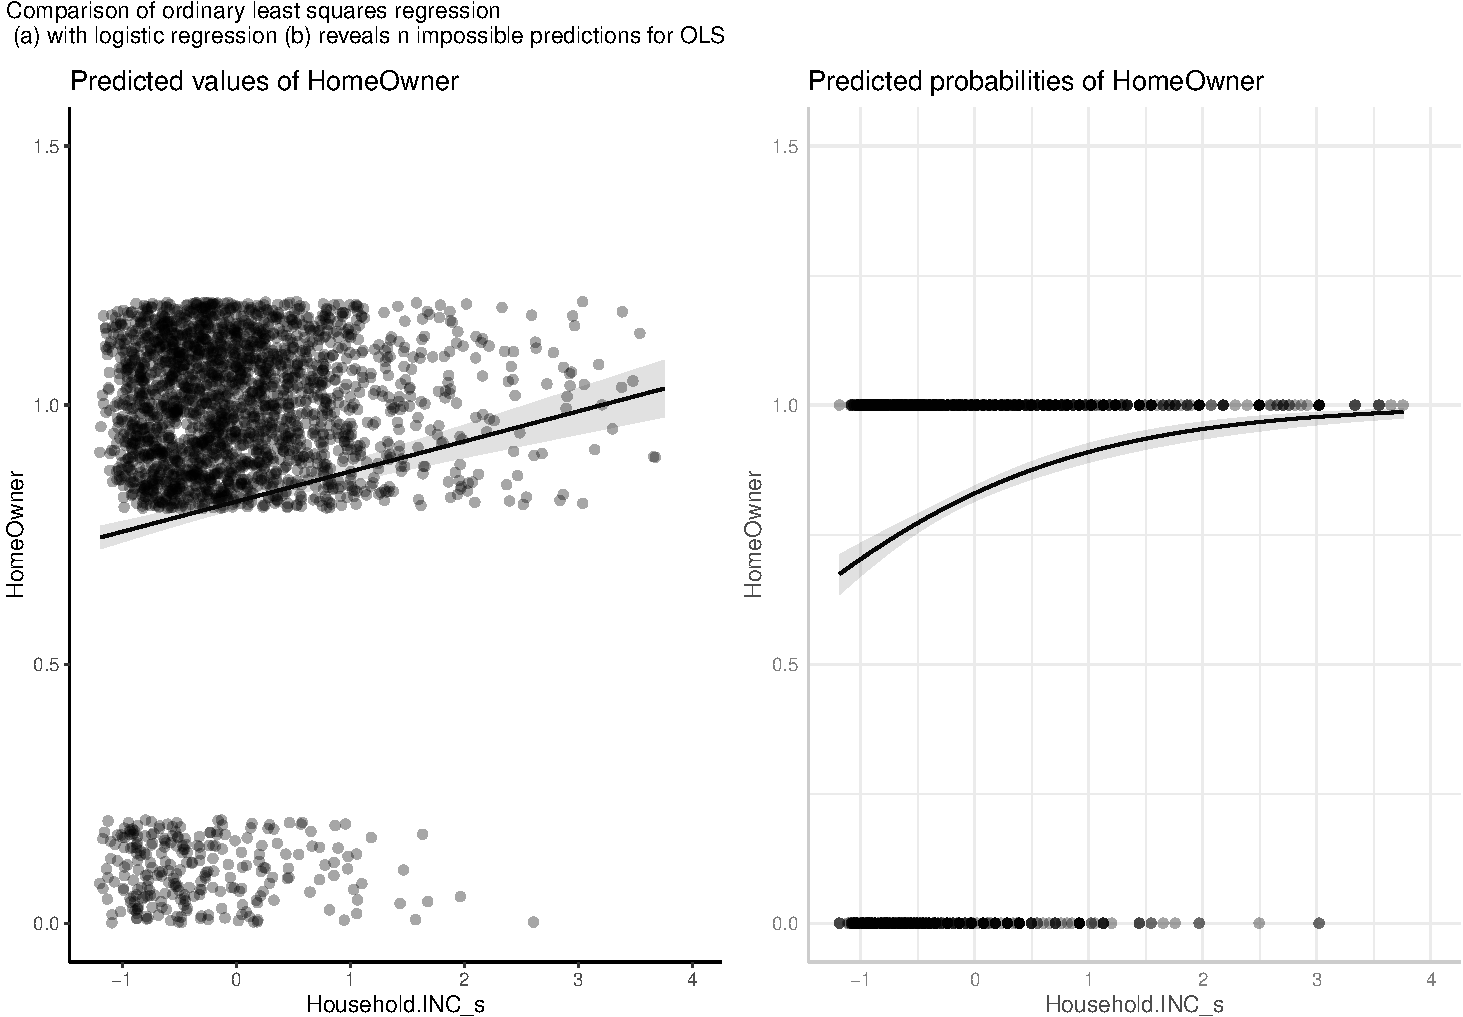
\includegraphics{slides_files/figure-beamer/unnamed-chunk-20-2.pdf}
\end{block}

\begin{block}{Logistic regression with a categorical covariate}
\protect\hypertarget{logistic-regression-with-a-categorical-covariate}{}
\begin{verbatim}
## Parameter                               | Log-Odds |   SE |         95% CI |      z |      p
## --------------------------------------------------------------------------------------------
## (Intercept)                             |     2.13 | 0.10 | [ 1.94,  2.34] |  20.68 | < .001
## GenCohortGen_Silent *  born< 1946       |     0.26 | 0.28 | [-0.26,  0.85] |   0.94 | 0.347 
## GenCohortGenX *  born >=1961 & b.< 1980 |    -0.62 | 0.13 | [-0.87, -0.38] |  -4.90 | < .001
## GenCohortGenY *  born >=1980 & b.< 1996 |    -1.87 | 0.14 | [-2.15, -1.59] | -13.00 | < .001
## GenCohortGenZ *  born >= 1996           |    -4.91 | 1.04 | [-7.80, -3.30] |  -4.74 | < .001
\end{verbatim}
\end{block}

\begin{block}{Interpretation}
\protect\hypertarget{interpretation}{}
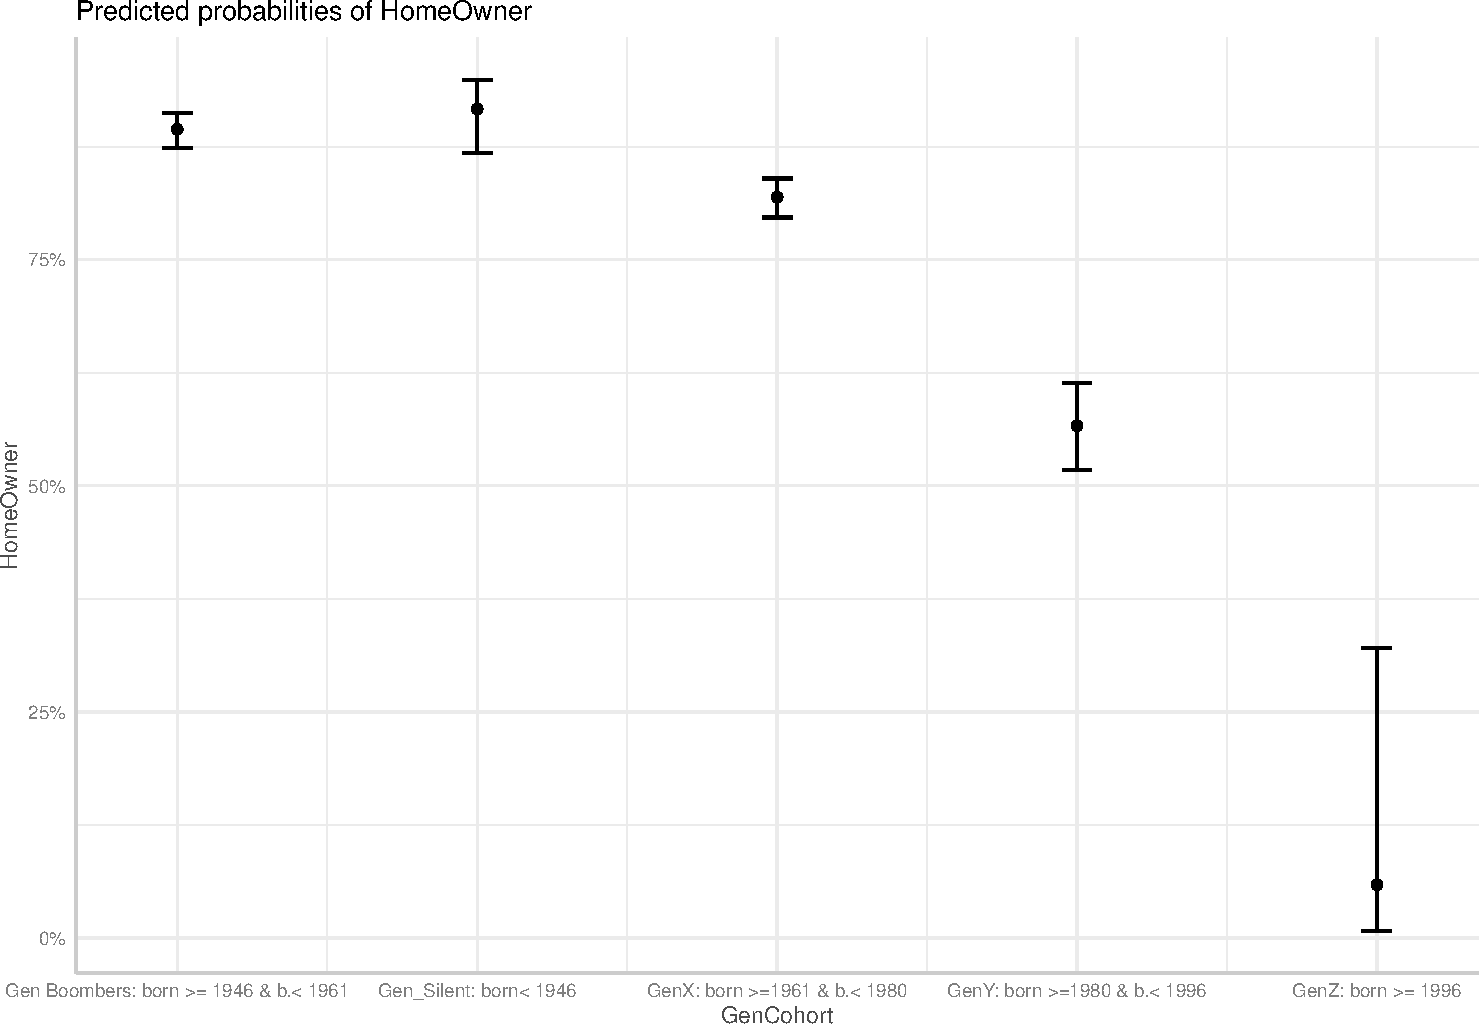
\includegraphics{slides_files/figure-beamer/unnamed-chunk-22-1.pdf}
\end{block}

\begin{block}{Stratify by income}
\protect\hypertarget{stratify-by-income}{}
\begin{verbatim}
## Parameter                               | Log-Odds |   SE |         95% CI |      z |      p
## --------------------------------------------------------------------------------------------
## (Intercept)                             |     2.60 | 0.12 | [ 2.37,  2.84] |  21.79 | < .001
## GenCohortGen_Silent *  born< 1946       |     0.70 | 0.30 | [ 0.15,  1.33] |   2.35 | 0.019 
## GenCohortGenX *  born >=1961 & b.< 1980 |    -0.99 | 0.14 | [-1.26, -0.73] |  -7.31 | < .001
## GenCohortGenY *  born >=1980 & b.< 1996 |    -2.40 | 0.16 | [-2.71, -2.09] | -14.94 | < .001
## GenCohortGenZ *  born >= 1996           |    -4.99 | 1.06 | [-7.91, -3.32] |  -4.72 | < .001
## Household.INC_s                         |     1.19 | 0.10 | [ 0.99,  1.39] |  11.62 | < .001
\end{verbatim}
\end{block}

\begin{block}{Results}
\protect\hypertarget{results-1}{}
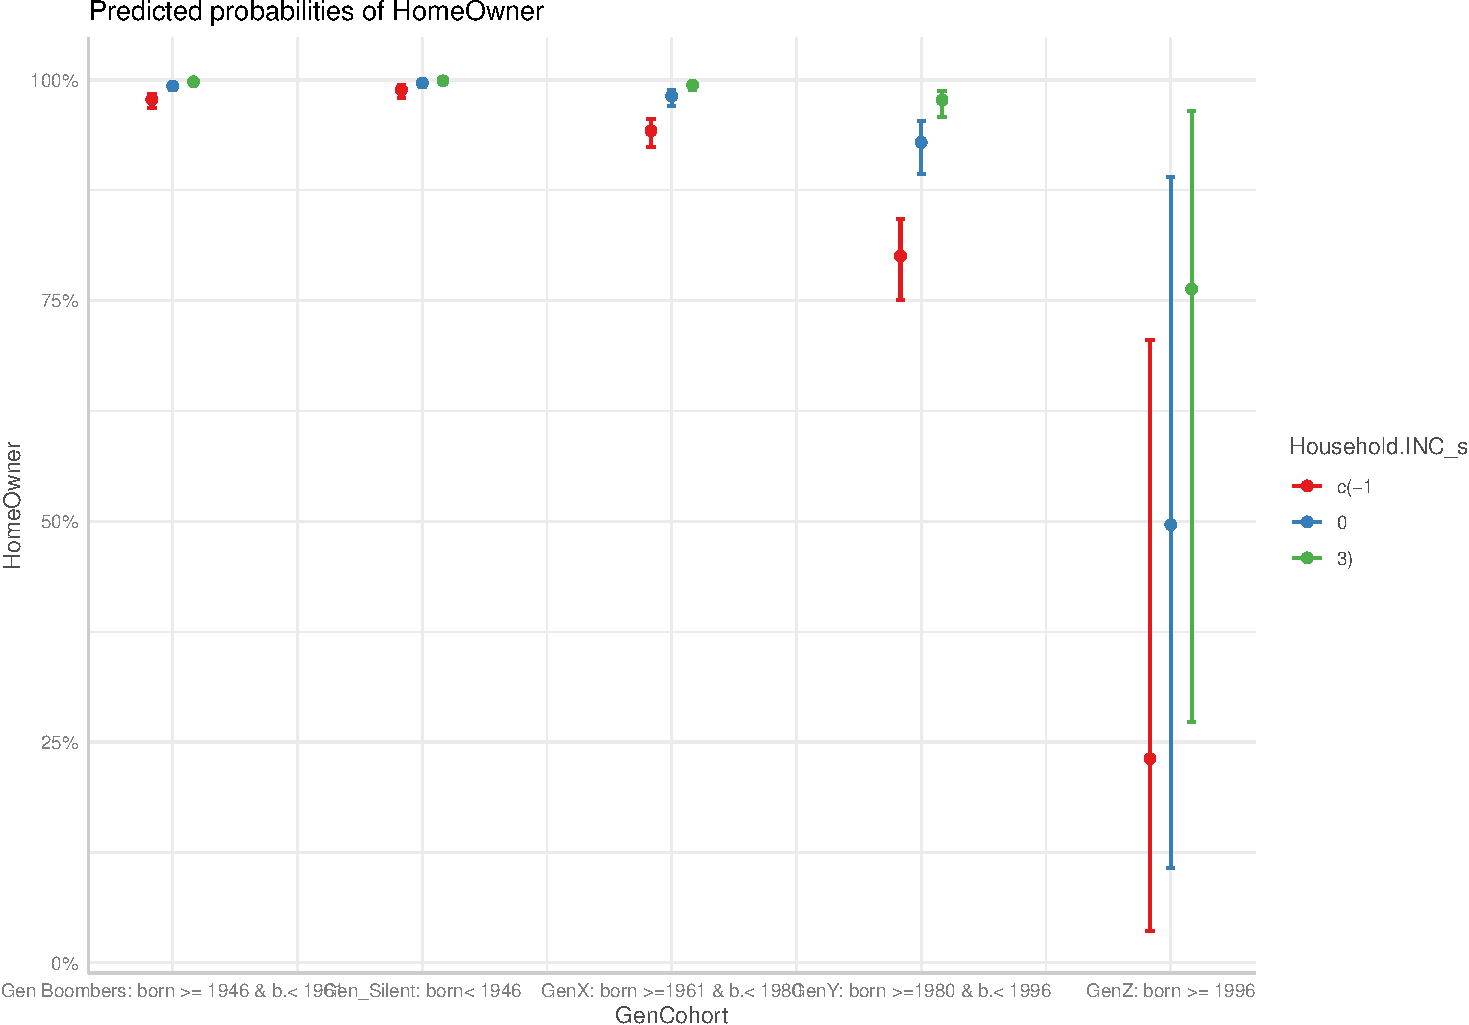
\includegraphics{slides_files/figure-beamer/unnamed-chunk-24-1.pdf}
\end{block}

\begin{block}{Add data to graph}
\protect\hypertarget{add-data-to-graph}{}
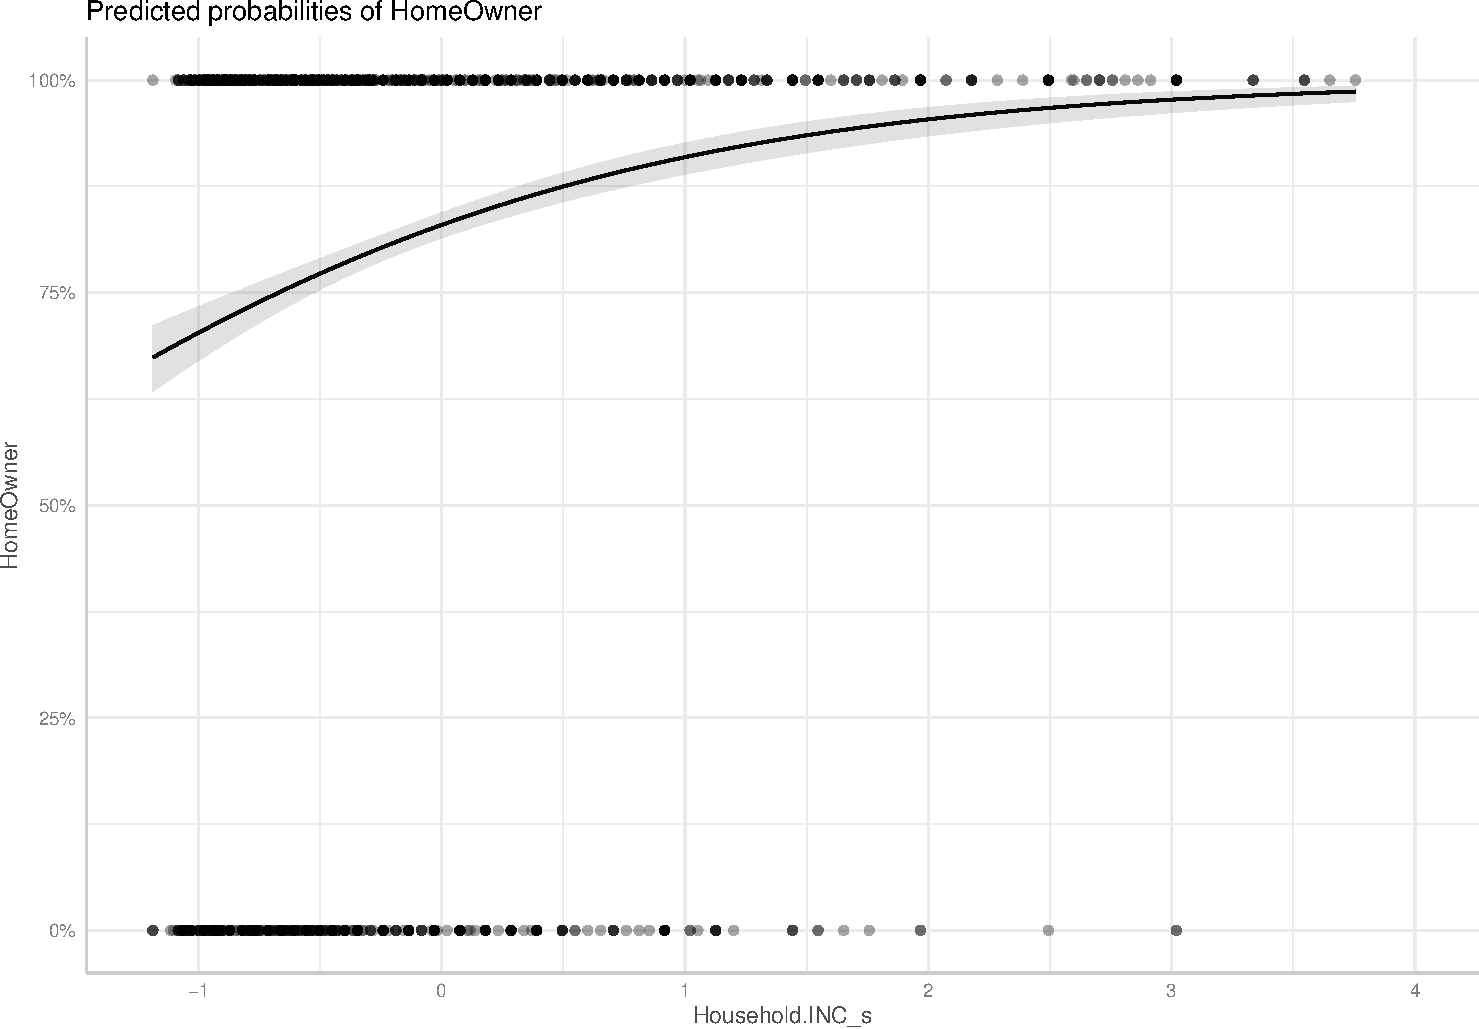
\includegraphics{slides_files/figure-beamer/unnamed-chunk-25-1.pdf}
\end{block}

\begin{block}{Counts in cells}
\protect\hypertarget{counts-in-cells}{}
\begin{verbatim}
## 
## Gen Boombers: born >= 1946 & b.< 1961                Gen_Silent: born< 1946 
##                                  1024                                   208 
##          GenX: born >=1961 & b.< 1980          GenY: born >=1980 & b.< 1996 
##                                  1253                                   416 
##                    GenZ: born >= 1996 
##                                    17
\end{verbatim}
\end{block}

\begin{block}{Graph}
\protect\hypertarget{graph}{}
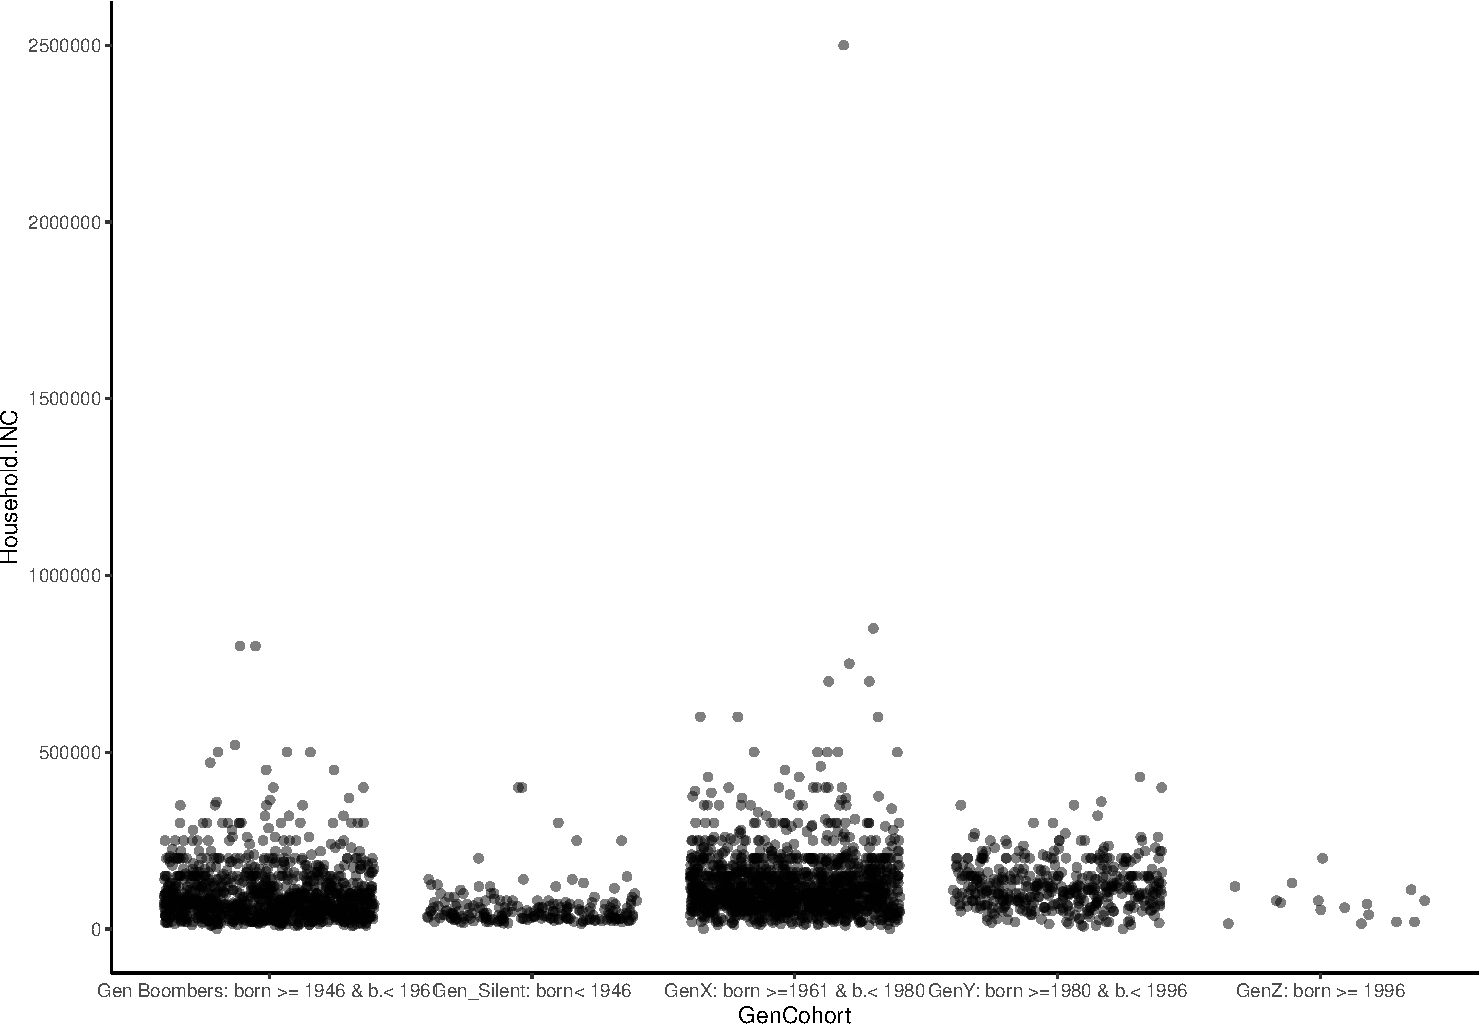
\includegraphics{slides_files/figure-beamer/unnamed-chunk-27-1.pdf}
\end{block}

\begin{block}{Model selection}
\protect\hypertarget{model-selection}{}
\begin{verbatim}
## # Comparison of Model Performance Indices
## 
## Name  | Model |      AIC |      BIC | Tjur's R2 |  RMSE | Sigma | Log_loss | Score_log |   PCP | Score_spherical
## ----------------------------------------------------------------------------------------------------------------
## home2 |   glm | 2590.320 | 2602.193 |     0.036 | 0.381 | 0.962 |    0.462 |      -Inf | 0.708 |                
## mg1   |   glm | 2516.922 | 2546.675 |     0.099 | 0.372 | 0.941 |    0.442 |      -Inf | 0.724 |       3.915e-04
## mg2   |   glm | 2272.307 | 2307.927 |     0.168 | 0.354 | 0.900 |    0.404 |      -Inf | 0.748 |       5.159e-04
\end{verbatim}
\end{block}

\begin{block}{Graph}
\protect\hypertarget{graph-1}{}
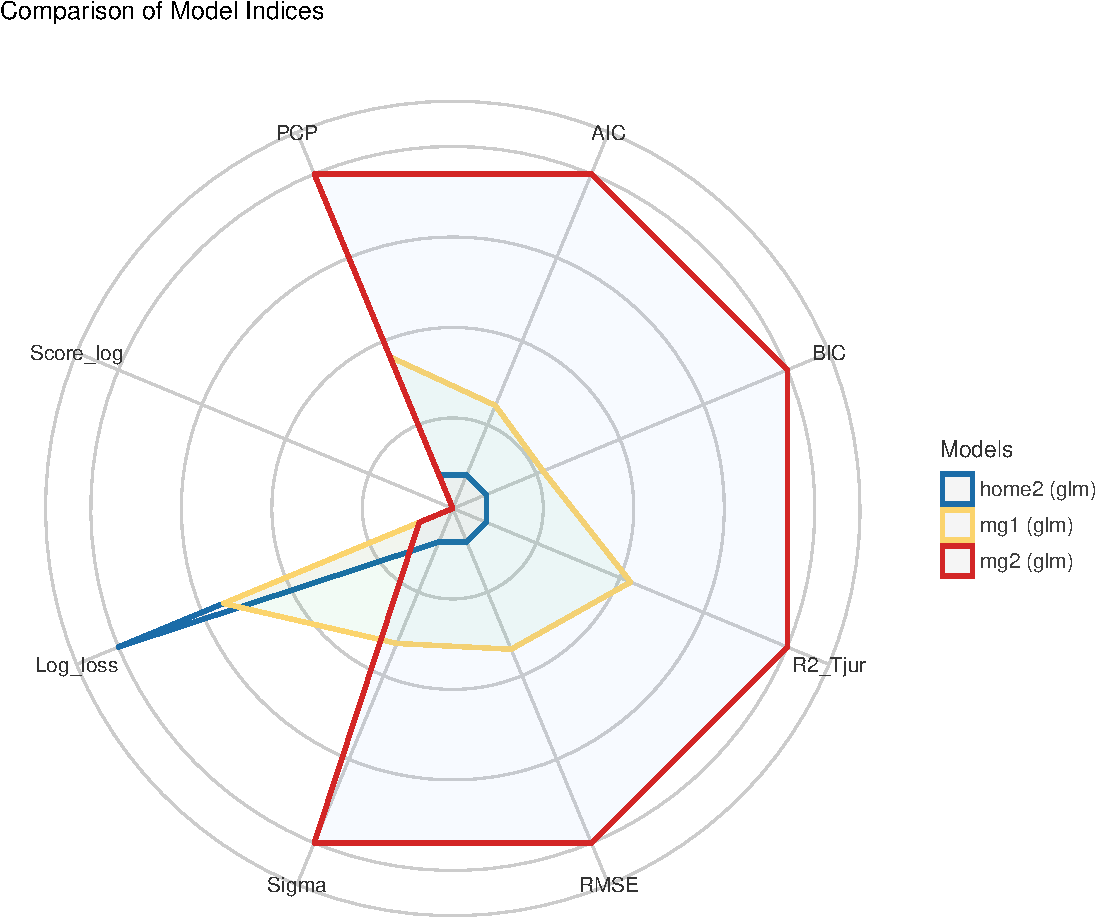
\includegraphics{slides_files/figure-beamer/unnamed-chunk-29-1.pdf}
\end{block}

\begin{block}{Model accuracy: model 1}
\protect\hypertarget{model-accuracy-model-1}{}
\begin{verbatim}
## # Accuracy of Model Predictions
## 
## Accuracy: 66.56%
##       SE: 2.26%-points
##   Method: Area under Curve
\end{verbatim}
\end{block}

\begin{block}{Model accuracy: model 2}
\protect\hypertarget{model-accuracy-model-2}{}
\begin{verbatim}
## # Accuracy of Model Predictions
## 
## Accuracy: 77.03%
##       SE: 1.94%-points
##   Method: Area under Curve
\end{verbatim}
\end{block}
\end{frame}

\begin{frame}[fragile]{Poisson regression (counts)}
\protect\hypertarget{poisson-regression-counts}{}
\begin{block}{Link function for poisson regression}
\protect\hypertarget{link-function-for-poisson-regression}{}
\[
y_i \sim Poisson(\lambda_i)\\  
log(\lambda_i) = \alpha +\beta x_i\\
E(\lambda|y_i) = exp(\alpha +\beta x_i)
\]
\end{block}

\begin{block}{Example}
\protect\hypertarget{example}{}
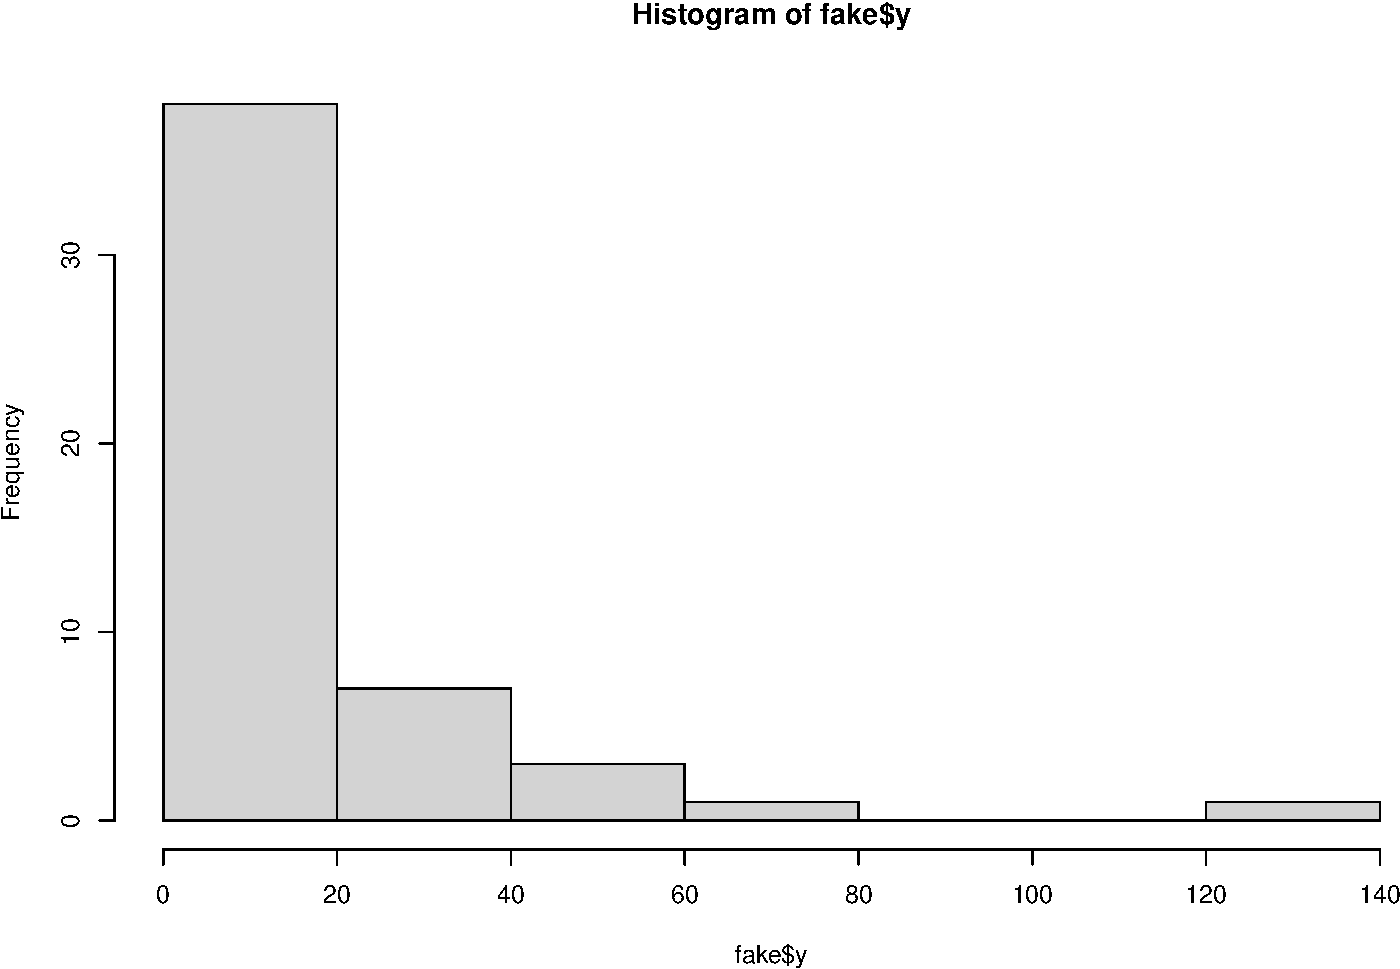
\includegraphics{slides_files/figure-beamer/unnamed-chunk-32-1.pdf}
\end{block}

\begin{block}{Model syntax}
\protect\hypertarget{model-syntax-1}{}
\begin{verbatim}
## Parameter   | Log-Mean |   SE |       95% CI |     z |      p
## -------------------------------------------------------------
## (Intercept) |     1.01 | 0.11 | [0.79, 1.21] |  9.40 | < .001
## x           |     1.99 | 0.08 | [1.84, 2.14] | 26.24 | < .001
\end{verbatim}
\end{block}

\begin{block}{Results}
\protect\hypertarget{results-2}{}
\[
\log ({ \widehat{E( \operatorname{y} )} })  = 1.01 + 1.99(\operatorname{x})
\]
\end{block}

\begin{block}{Graph}
\protect\hypertarget{graph-2}{}
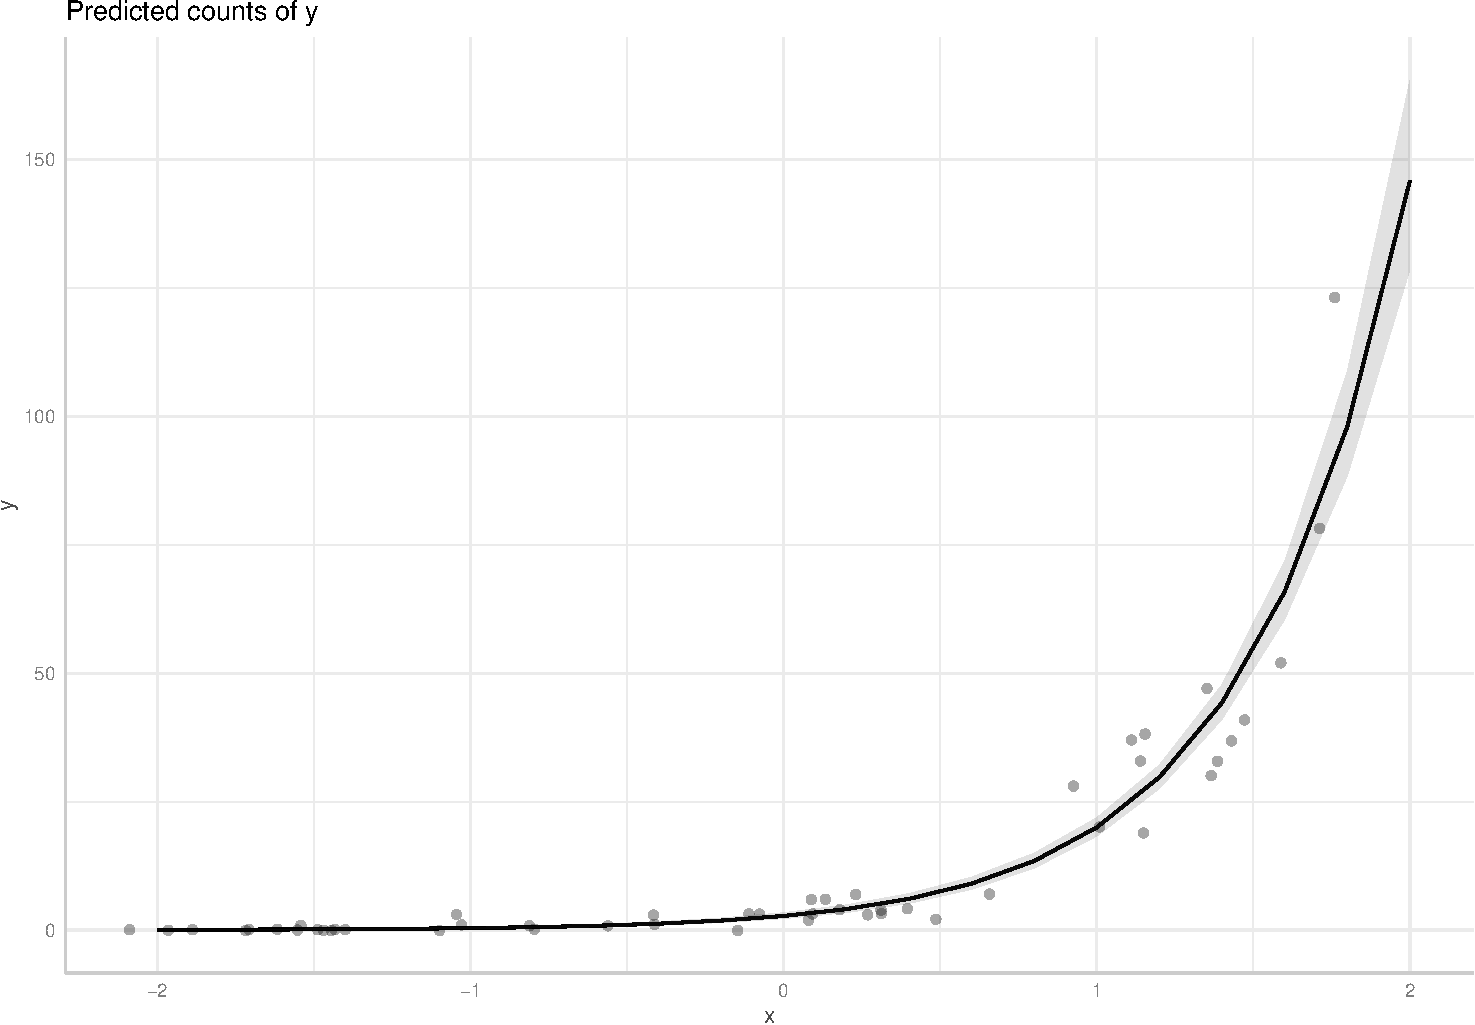
\includegraphics{slides_files/figure-beamer/unnamed-chunk-35-1.pdf}
\end{block}

\begin{block}{Compare with normal lm}
\protect\hypertarget{compare-with-normal-lm}{}
\begin{Shaded}
\begin{Highlighting}[]
\CommentTok{\# model}
\NormalTok{pois2 }\OtherTok{\textless{}{-}} \FunctionTok{glm}\NormalTok{(y }\SpecialCharTok{\textasciitilde{}}\NormalTok{ x, }\AttributeTok{data =}\NormalTok{ fake) }\CommentTok{\# remove "family = \textasciigrave{}poisson\textasciigrave{})}
\CommentTok{\# graph }
\NormalTok{p\_pois2 }\OtherTok{\textless{}{-}} \FunctionTok{plot}\NormalTok{(ggeffects}\SpecialCharTok{::}\FunctionTok{ggpredict}\NormalTok{(pois2, }\AttributeTok{terms =} \StringTok{"x"}\NormalTok{),}
                \AttributeTok{add.data =} \ConstantTok{TRUE}\NormalTok{)}
\CommentTok{\# render}
\NormalTok{p\_pois2}
\end{Highlighting}
\end{Shaded}

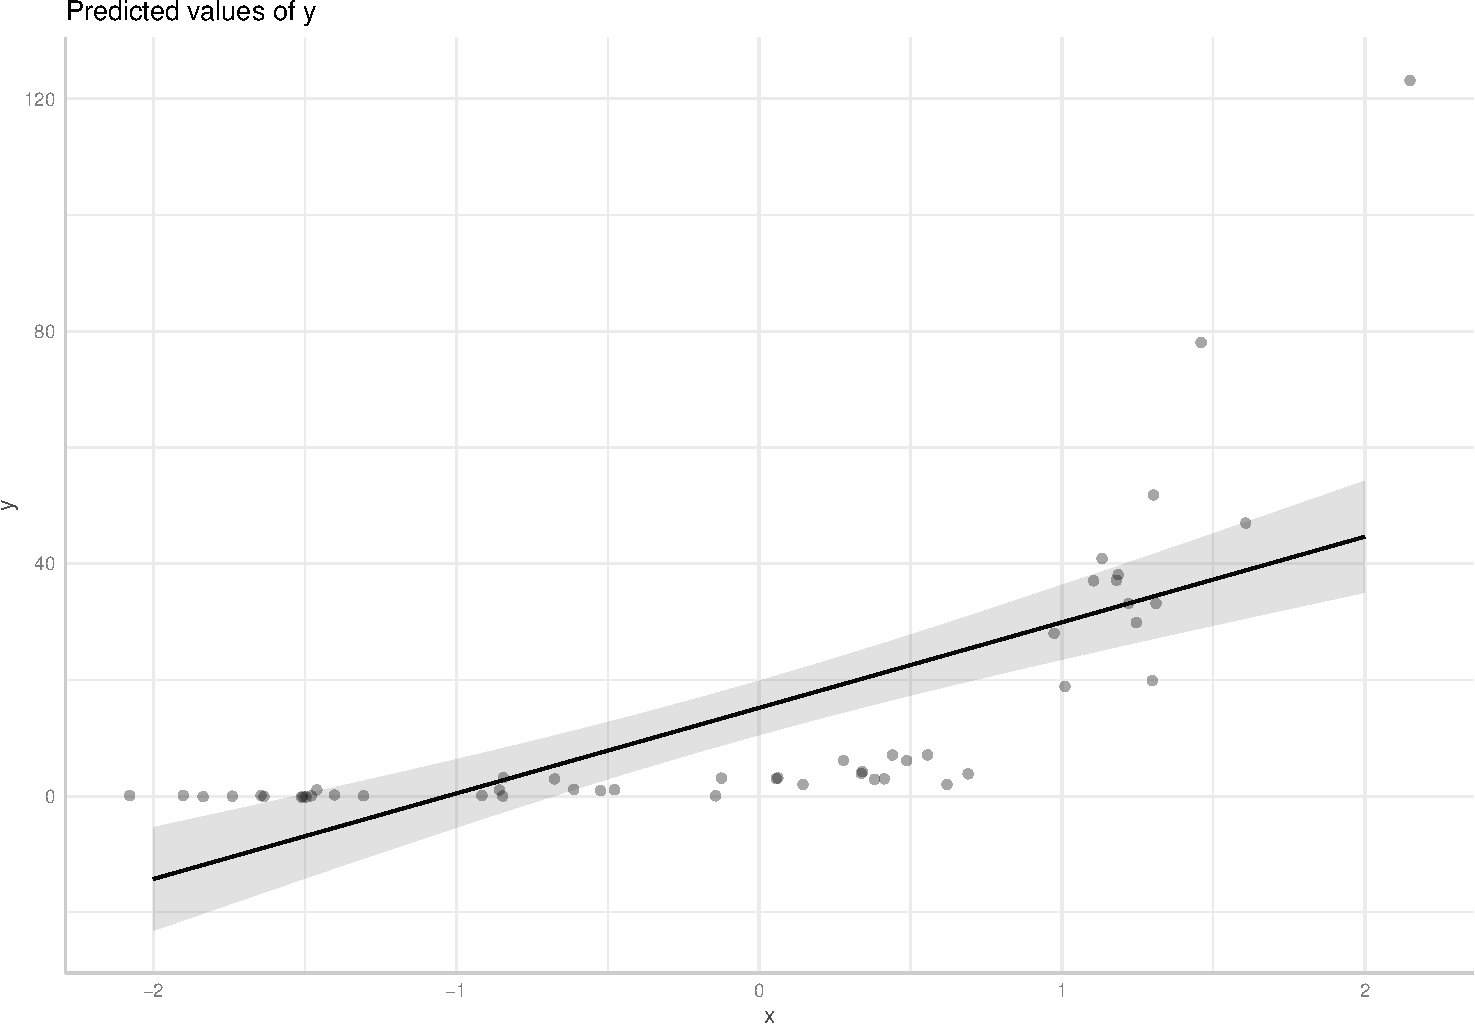
\includegraphics{slides_files/figure-beamer/unnamed-chunk-36-1.pdf}
\end{block}
\end{frame}

\begin{frame}{Splines}
\protect\hypertarget{splines}{}
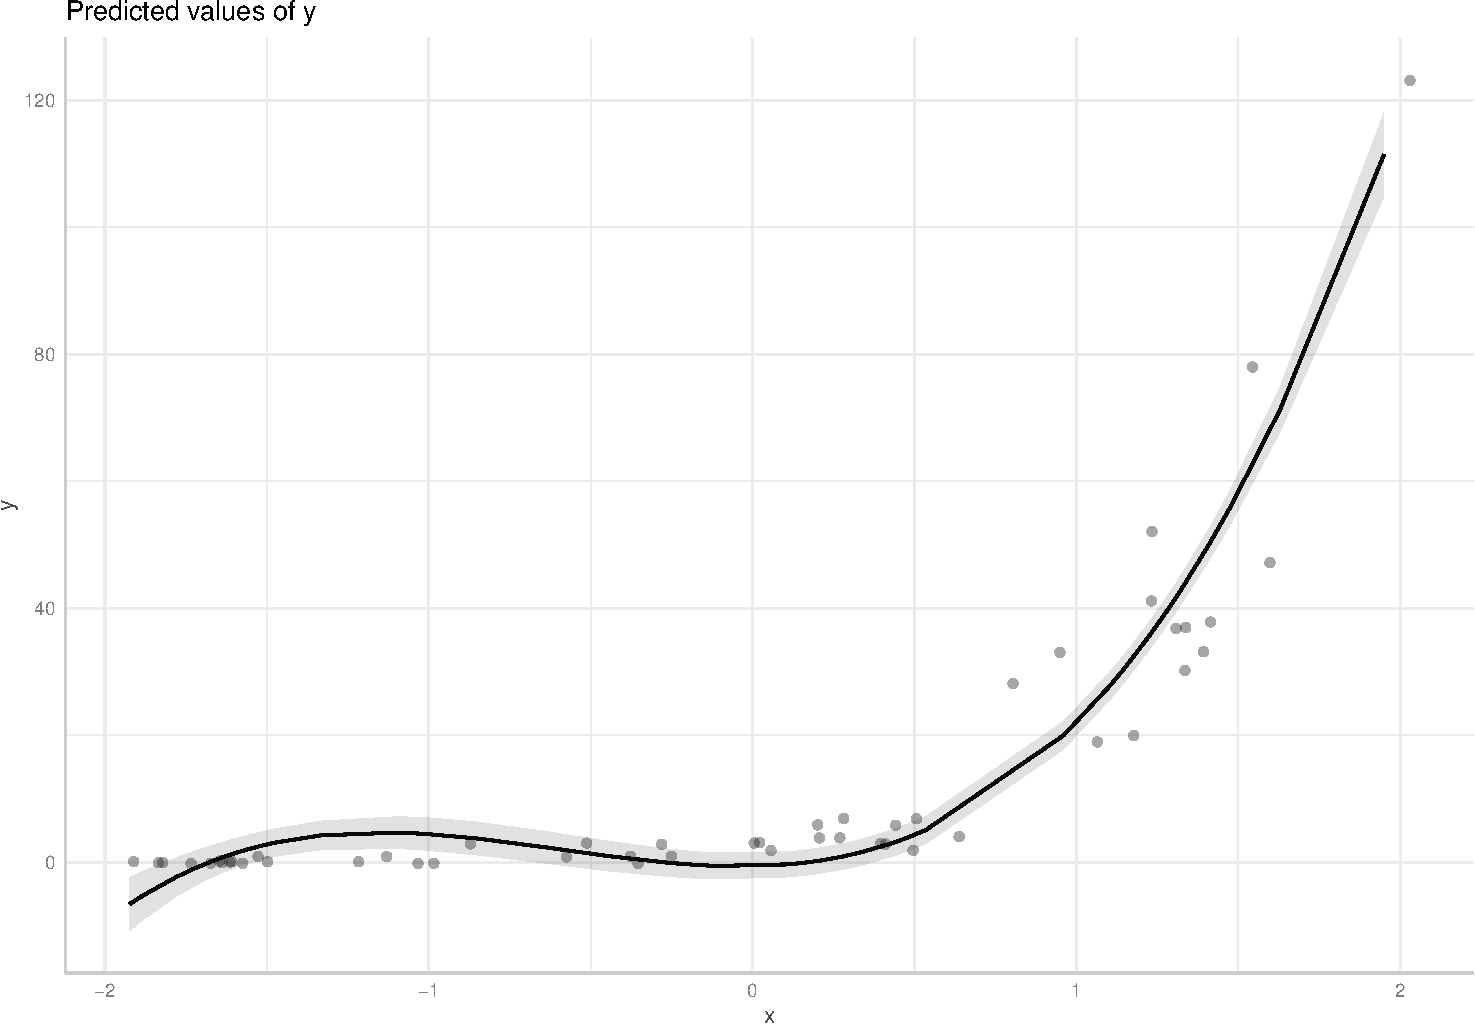
\includegraphics{slides_files/figure-beamer/unnamed-chunk-37-1.pdf}

\begin{block}{Graph all three}
\protect\hypertarget{graph-all-three}{}
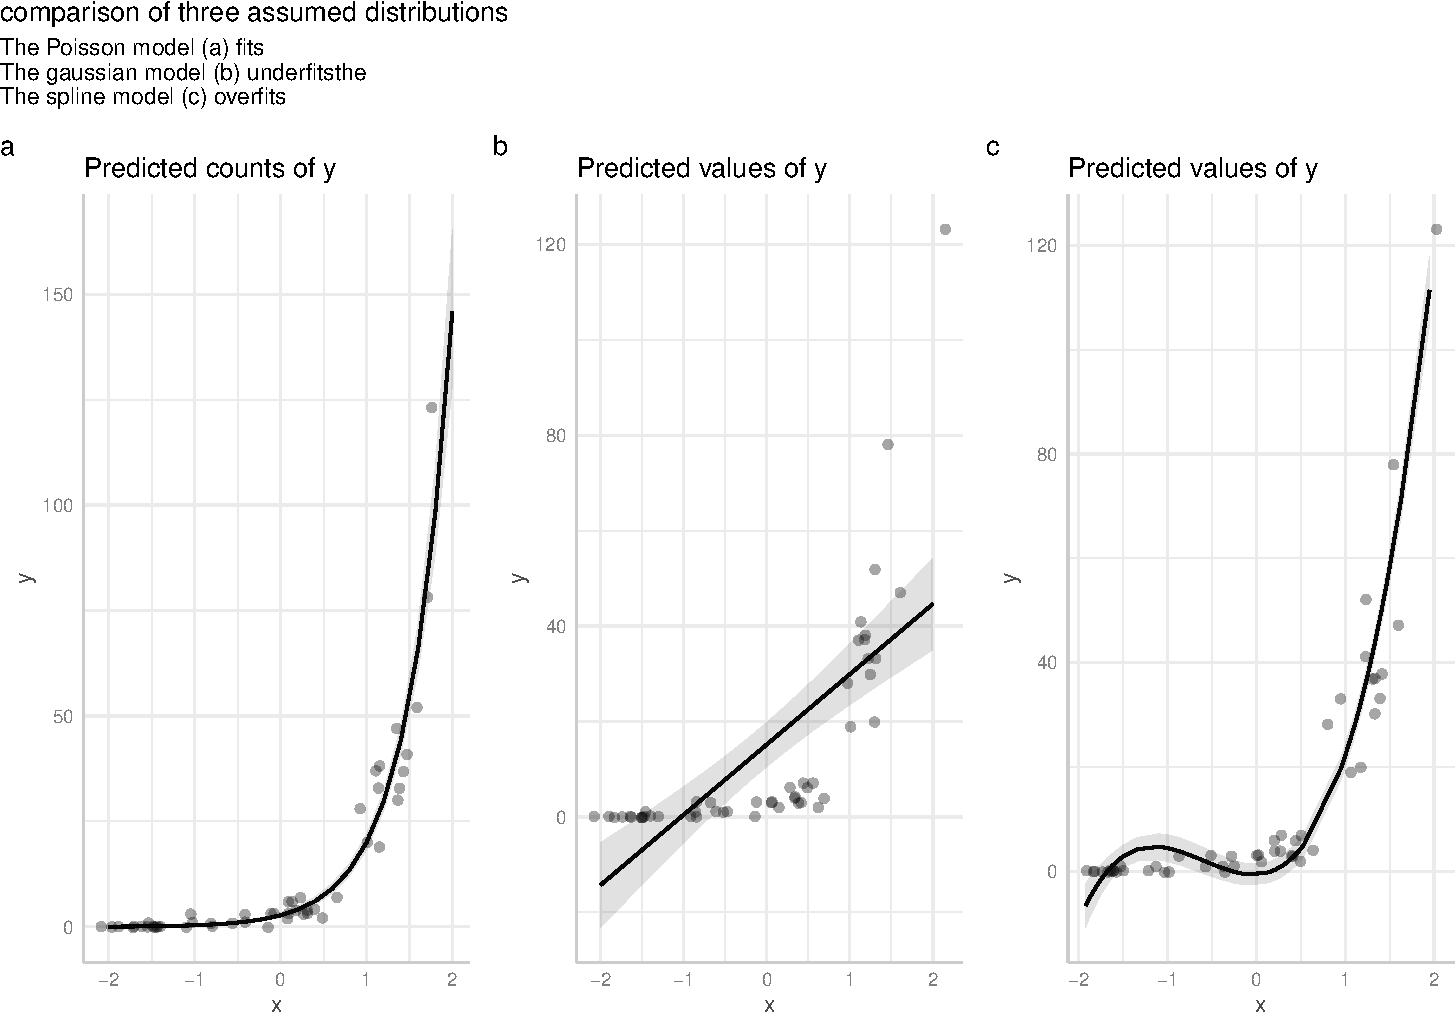
\includegraphics{slides_files/figure-beamer/unnamed-chunk-38-1.pdf}
\end{block}

\begin{block}{Compare performance}
\protect\hypertarget{compare-performance}{}
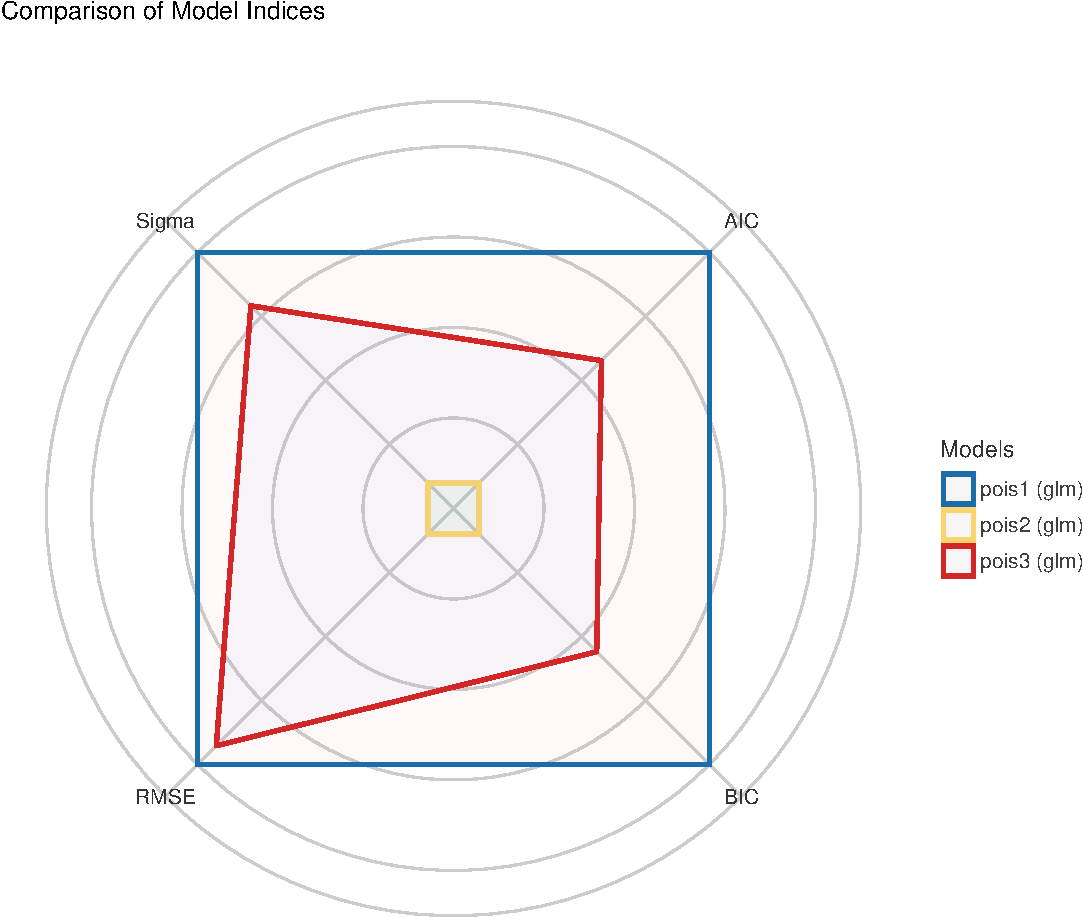
\includegraphics{slides_files/figure-beamer/unnamed-chunk-39-1.pdf}
\end{block}
\end{frame}

\begin{frame}[fragile]{Negative binomial models (over-dispersed
Poissons)}
\protect\hypertarget{negative-binomial-models-over-dispersed-poissons}{}
\begin{block}{Link function for a negative binomial model}
\protect\hypertarget{link-function-for-a-negative-binomial-model}{}
\[
y_i \sim NegBinomial(\lambda_i,\phi)\\
log(\lambda_i) = \alpha +\beta x_i\\
\phi \sim gamma(.01,.01)
\]
\end{block}

\begin{block}{Example data}
\protect\hypertarget{example-data}{}
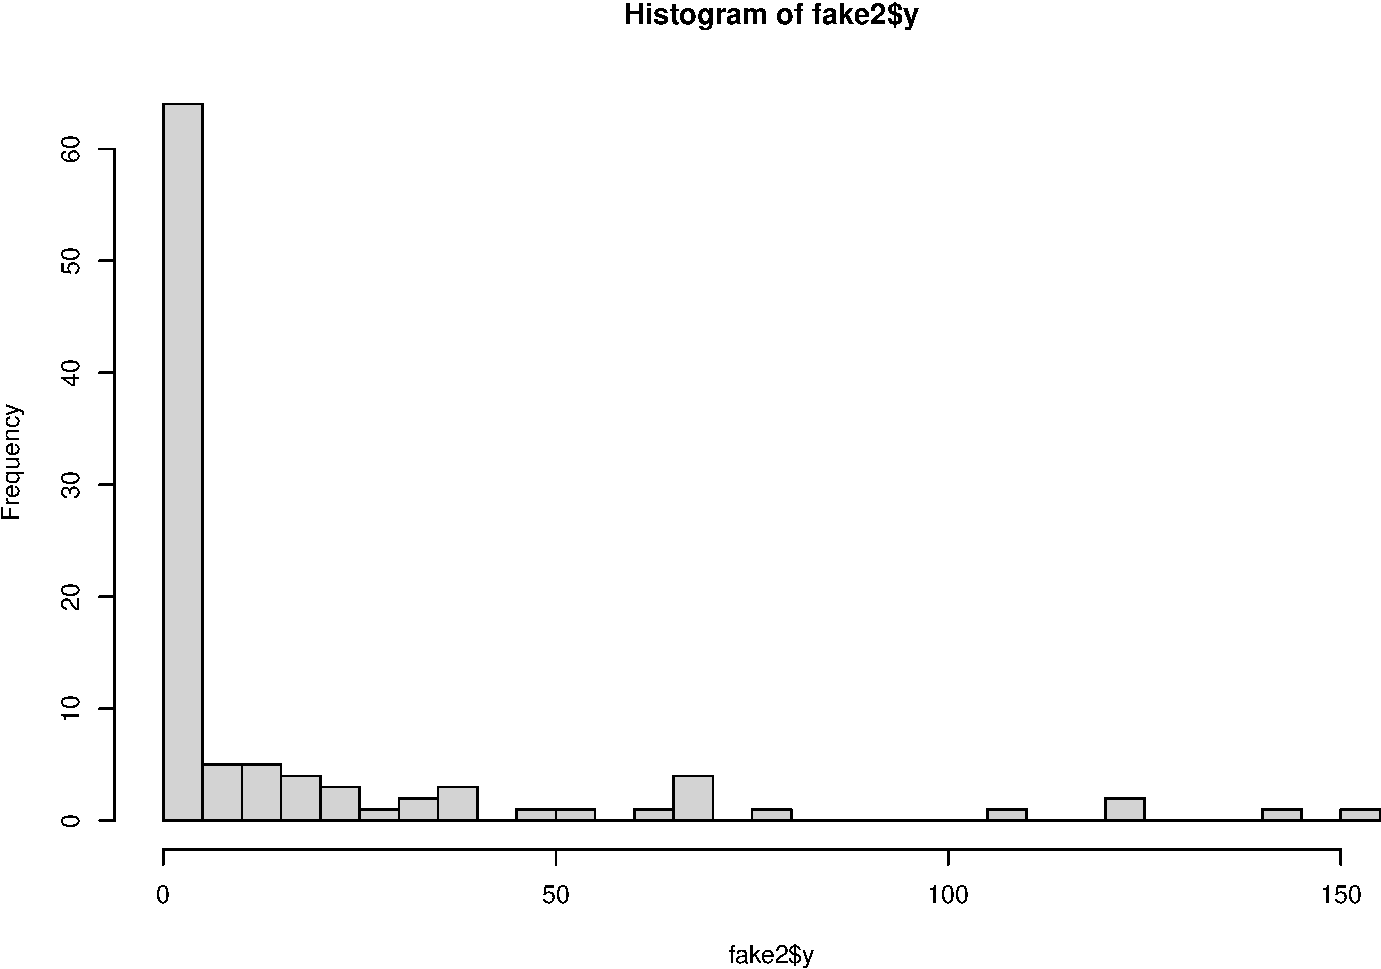
\includegraphics{slides_files/figure-beamer/unnamed-chunk-40-1.pdf}
\end{block}

\begin{block}{Fit model: poisson}
\protect\hypertarget{fit-model-poisson}{}
\begin{verbatim}
## # Overdispersion test
## 
##        dispersion ratio =   5.068
##   Pearson's Chi-Squared = 496.695
##                 p-value = < 0.001
\end{verbatim}
\end{block}

\begin{block}{Model syntax: neg.bin}
\protect\hypertarget{model-syntax-neg.bin}{}
\end{block}

\begin{block}{Graph poisson}
\protect\hypertarget{graph-poisson}{}
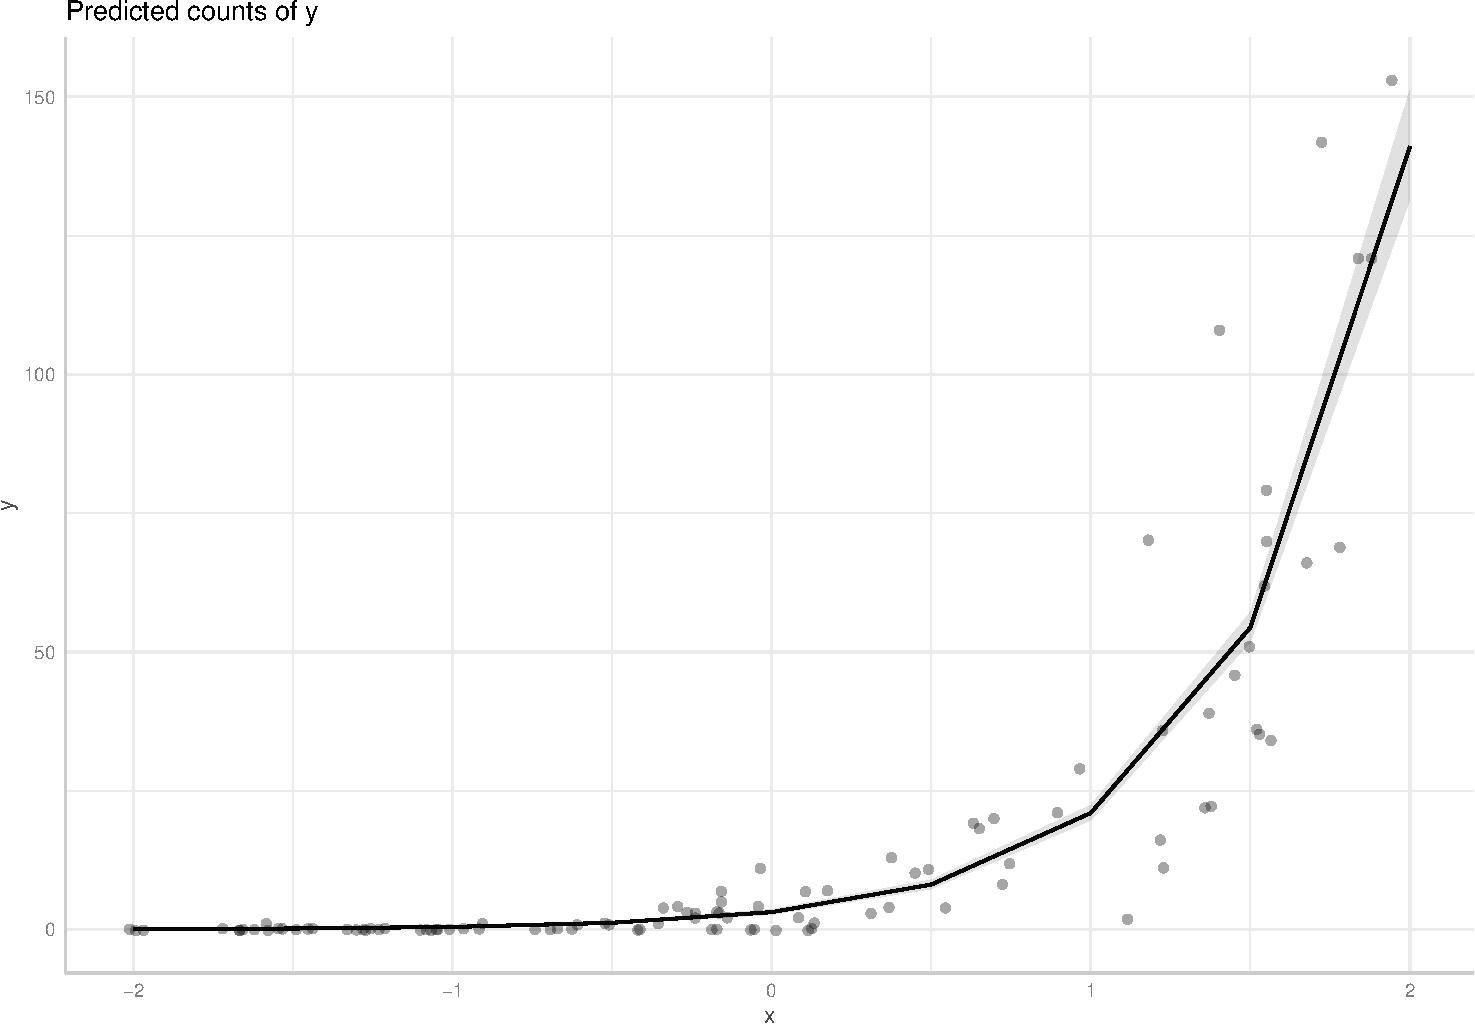
\includegraphics{slides_files/figure-beamer/unnamed-chunk-43-1.pdf}
\end{block}

\begin{block}{Graph negative binomial}
\protect\hypertarget{graph-negative-binomial}{}
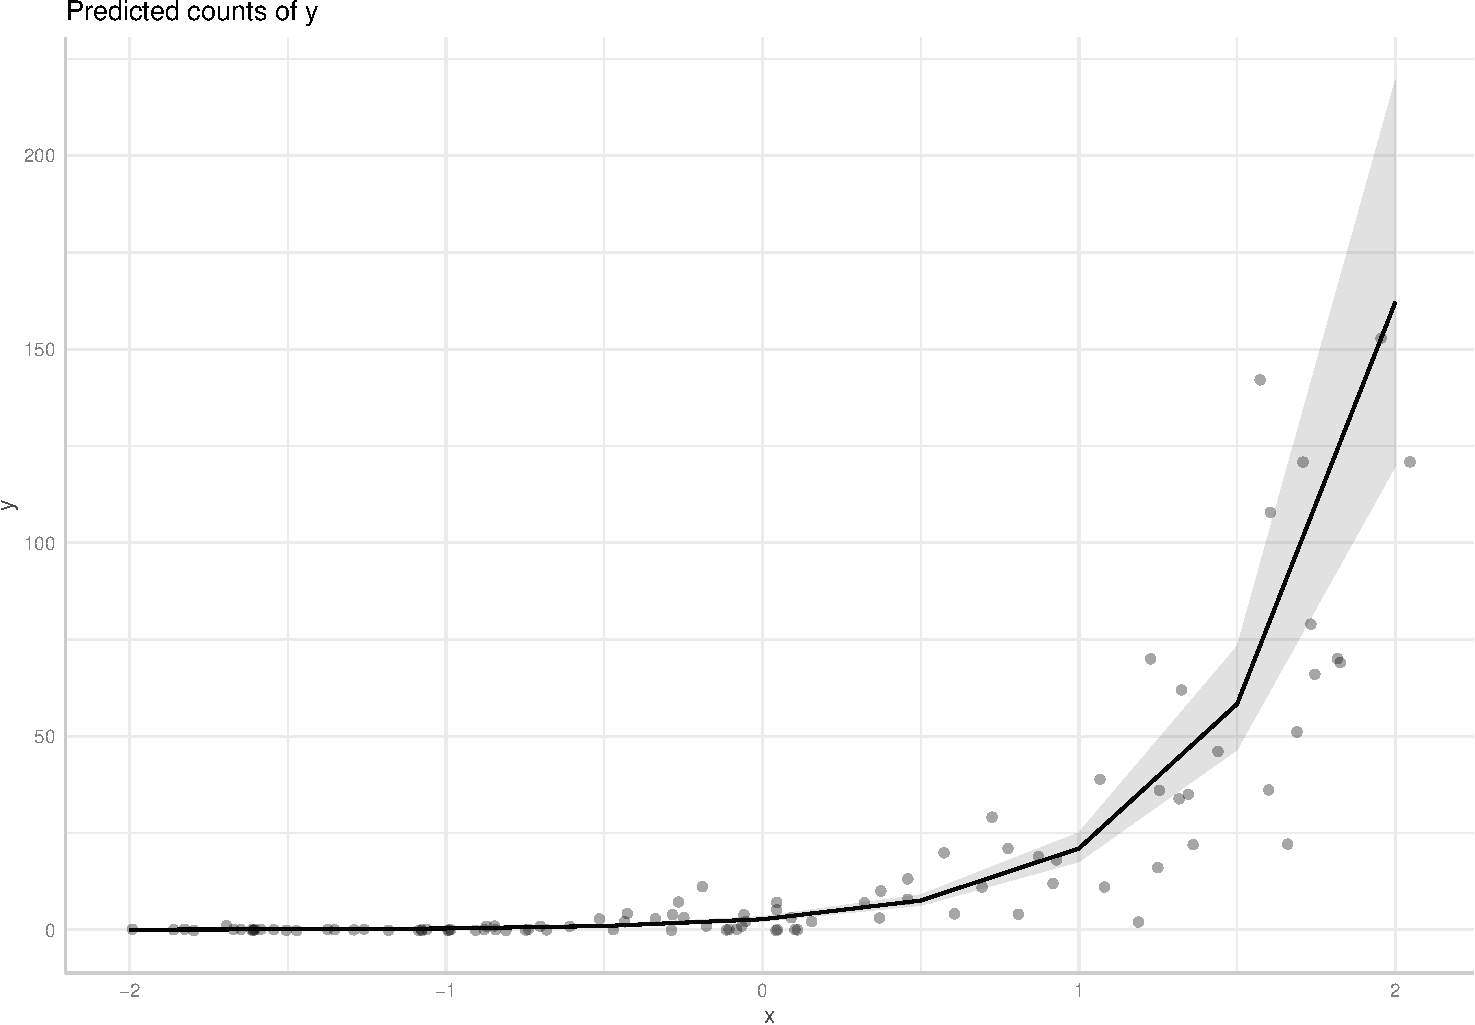
\includegraphics{slides_files/figure-beamer/unnamed-chunk-44-1.pdf}
\end{block}

\begin{block}{Linear model?}
\protect\hypertarget{linear-model}{}
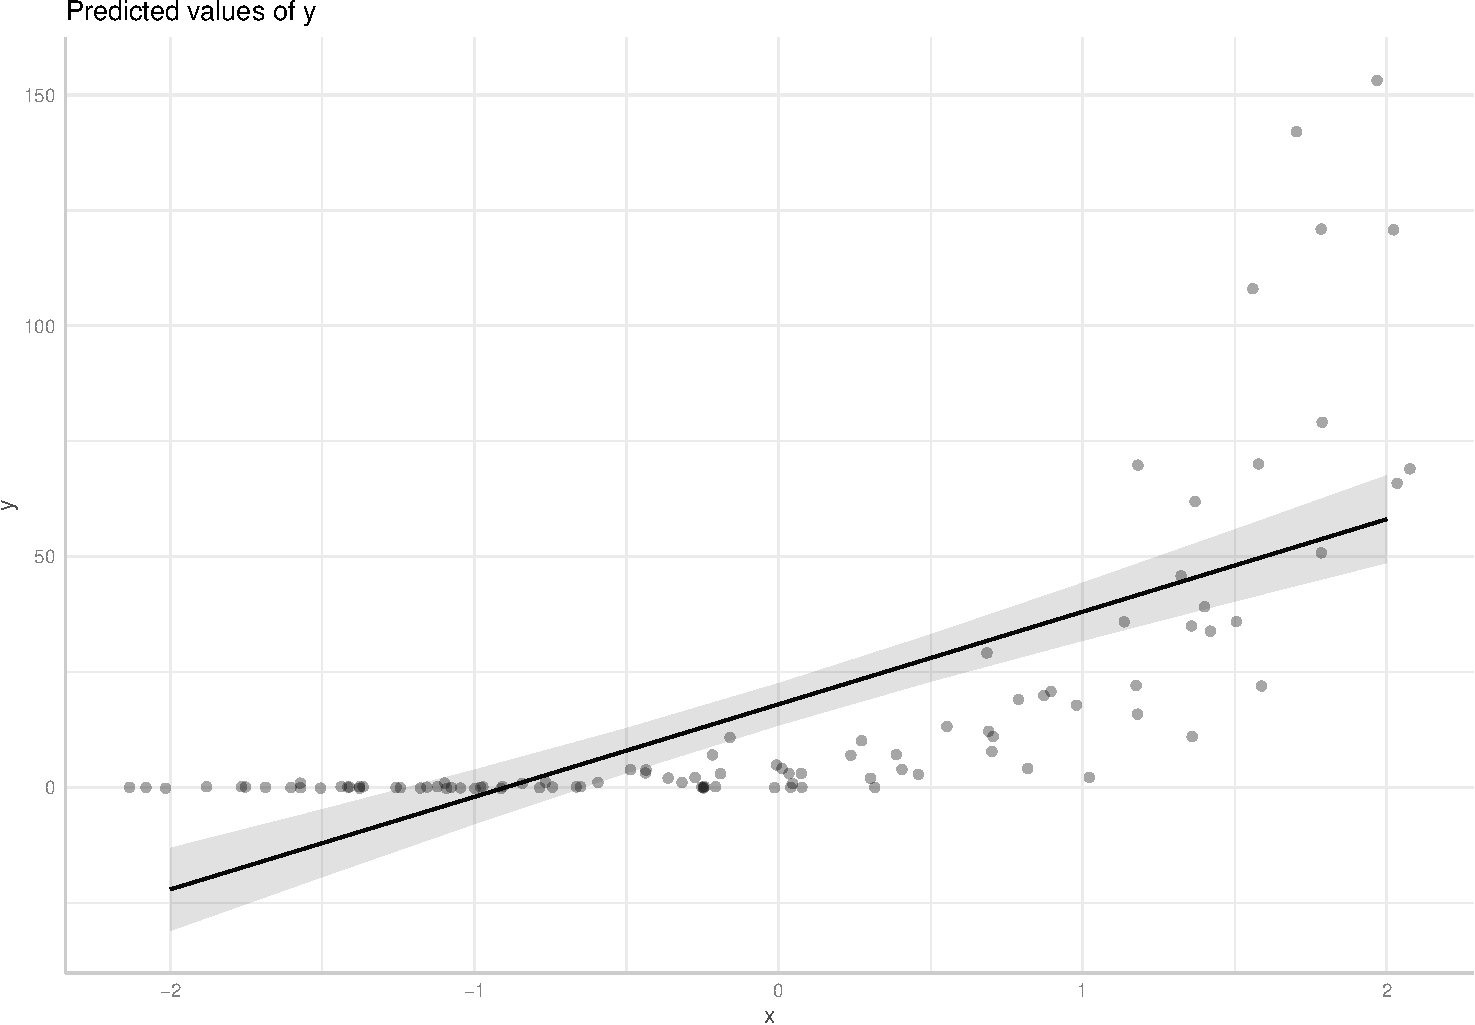
\includegraphics{slides_files/figure-beamer/unnamed-chunk-45-1.pdf}
\end{block}
\end{frame}

\begin{frame}[fragile]{Zero-inflated poisson/ neg binomial regression}
\protect\hypertarget{zero-inflated-poisson-neg-binomial-regression}{}
\begin{block}{Link function for zero-inflated poisson}
\protect\hypertarget{link-function-for-zero-inflated-poisson}{}
\[
y_i \sim ZIPoisson(p_i, \lambda_i)\\
logit(p_i) = \alpha_p + \beta_p x_i \\
log(\lambda) = \alpha_\lambda + \beta\lambda x_i
\]
\end{block}

\begin{block}{Example: hours volutneering}
\protect\hypertarget{example-hours-volutneering}{}
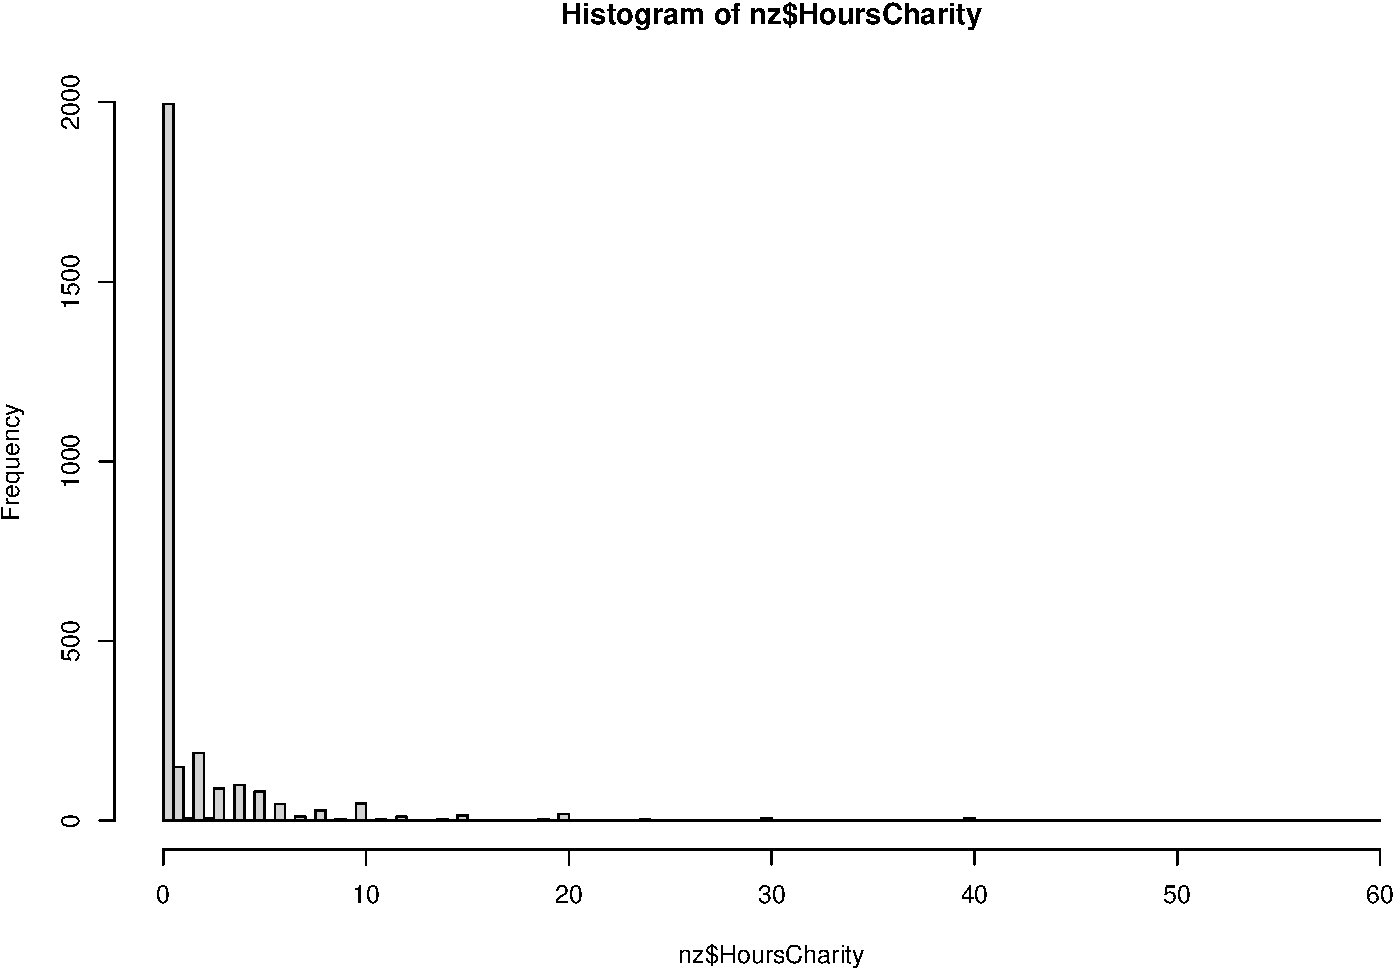
\includegraphics{slides_files/figure-beamer/unnamed-chunk-46-1.pdf}
\end{block}

\begin{block}{Proportion of non-volunteers}
\protect\hypertarget{proportion-of-non-volunteers}{}
\begin{verbatim}
## [1] 0.6826594
\end{verbatim}
\end{block}

\begin{block}{Crude estimate of overdispersion}
\protect\hypertarget{crude-estimate-of-overdispersion}{}
\begin{verbatim}
## [1] 1.680429
\end{verbatim}

There's about 1.68 more dispersion that a poisson model would expect
\end{block}

\begin{block}{Formal zero-inflation check}
\protect\hypertarget{formal-zero-inflation-check}{}
\begin{verbatim}
## # Check for zero-inflation
## 
##    Observed zeros: 1992
##   Predicted zeros: 536
##             Ratio: 0.27
\end{verbatim}
\end{block}

\begin{block}{Formal overdispersion check}
\protect\hypertarget{formal-overdispersion-check}{}
\begin{verbatim}
## # Overdispersion test
## 
##        dispersion ratio =    13.196
##   Pearson's Chi-Squared = 37595.179
##                 p-value =   < 0.001
\end{verbatim}
\end{block}

\begin{block}{Model syntax (\texttt{brms\ package})}
\protect\hypertarget{model-syntax-brms-package}{}
\end{block}

\begin{block}{Results}
\protect\hypertarget{results-3}{}
\begin{verbatim}
##  Family: zero_inflated_poisson 
##   Links: mu = log; zi = identity 
## Formula: HoursCharity ~ Relid_s + Household.INC_s 
##    Data: nz (Number of observations: 2796) 
## Samples: 4 chains, each with iter = 2000; warmup = 1000; thin = 1;
##          total post-warmup samples = 4000
## 
## Population-Level Effects: 
##                 Estimate Est.Error l-95% CI u-95% CI Rhat Bulk_ESS Tail_ESS
## Intercept           1.70      0.02     1.67     1.73 1.00     3785     3068
## Relid_s             0.00      0.01    -0.02     0.03 1.00     4501     3362
## Household.INC_s    -0.09      0.02    -0.12    -0.05 1.00     3704     3054
## 
## Family Specific Parameters: 
##    Estimate Est.Error l-95% CI u-95% CI Rhat Bulk_ESS Tail_ESS
## zi     0.70      0.01     0.68     0.72 1.00     3849     2989
## 
## Samples were drawn using sampling(NUTS). For each parameter, Bulk_ESS
## and Tail_ESS are effective sample size measures, and Rhat is the potential
## scale reduction factor on split chains (at convergence, Rhat = 1).
\end{verbatim}
\end{block}

\begin{block}{Predicted effects of religion}
\protect\hypertarget{predicted-effects-of-religion}{}
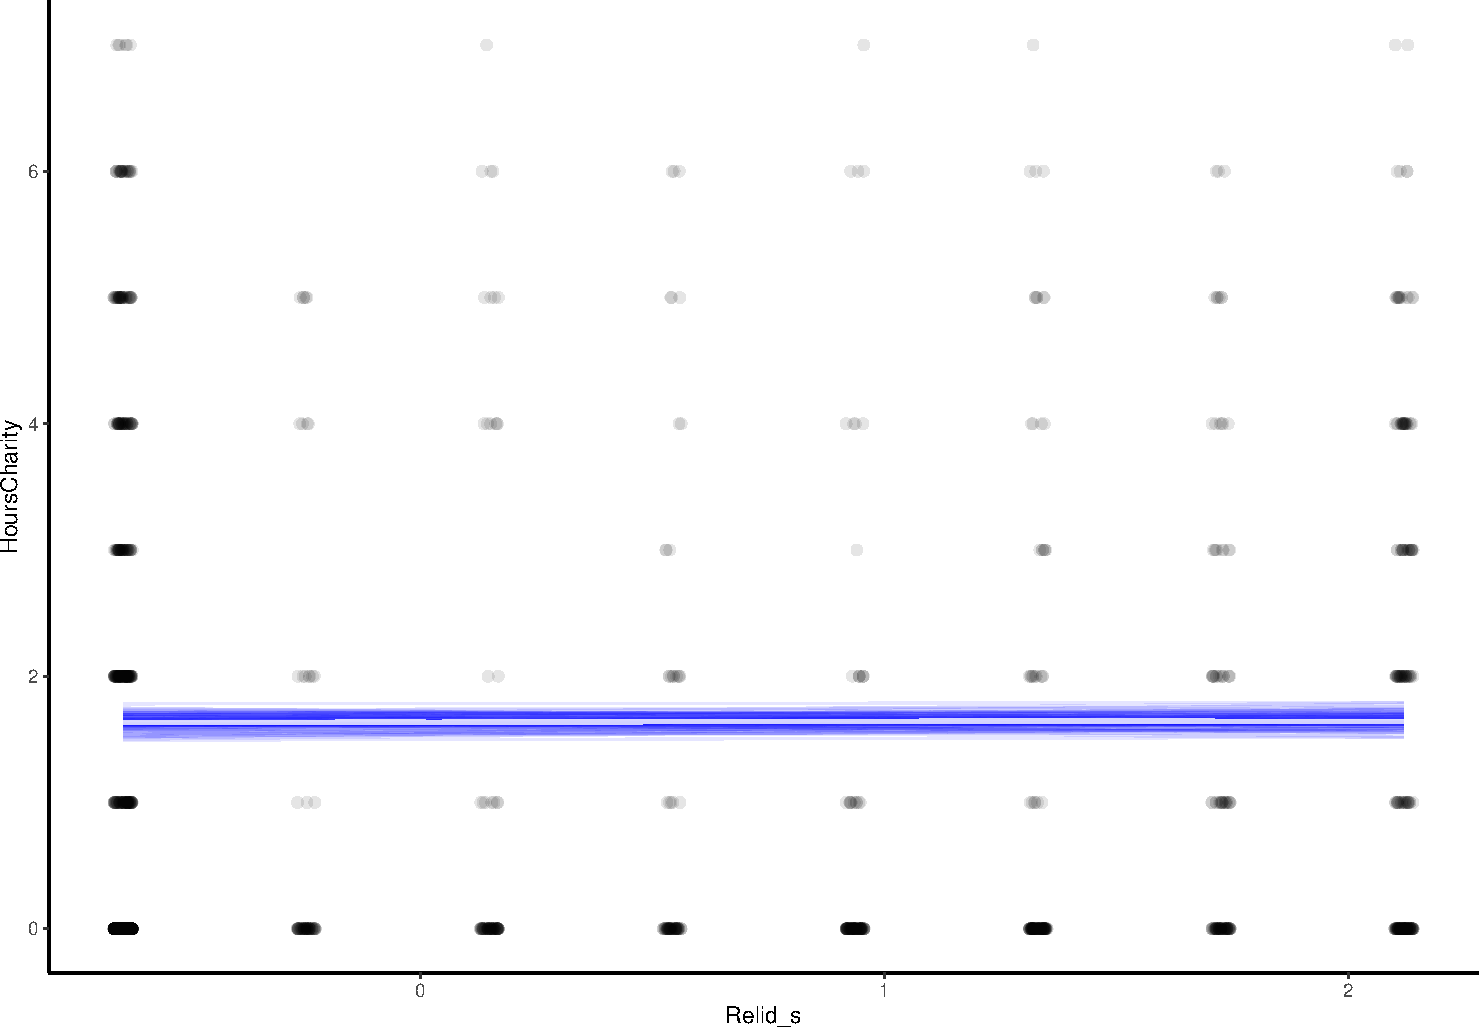
\includegraphics{slides_files/figure-beamer/unnamed-chunk-54-1.pdf}
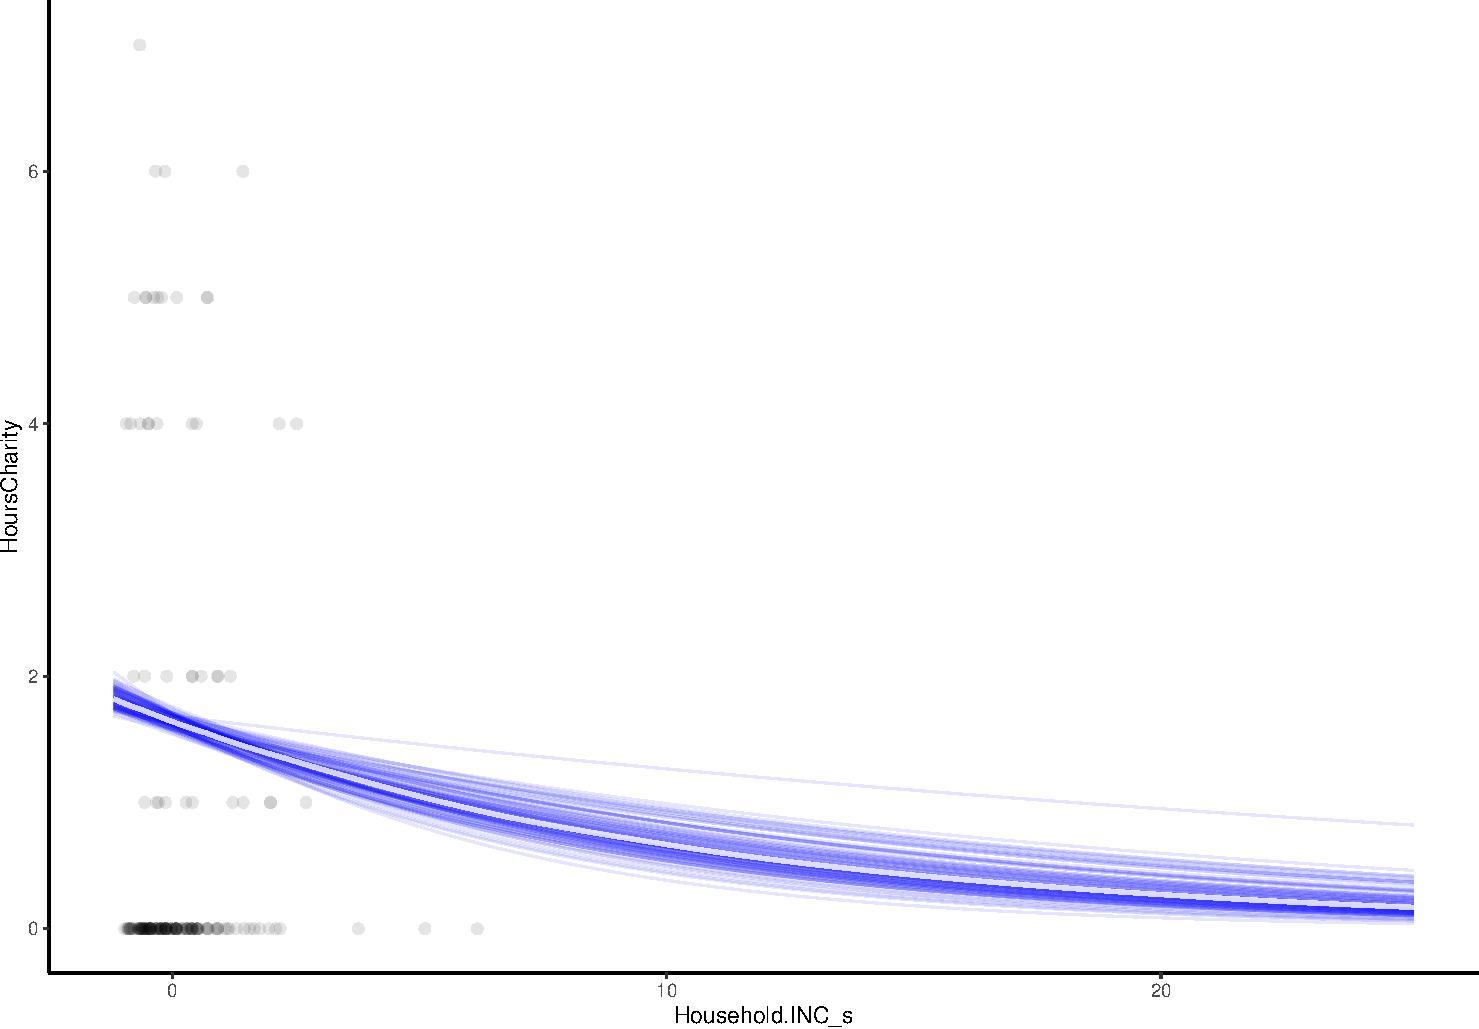
\includegraphics{slides_files/figure-beamer/unnamed-chunk-54-2.pdf}
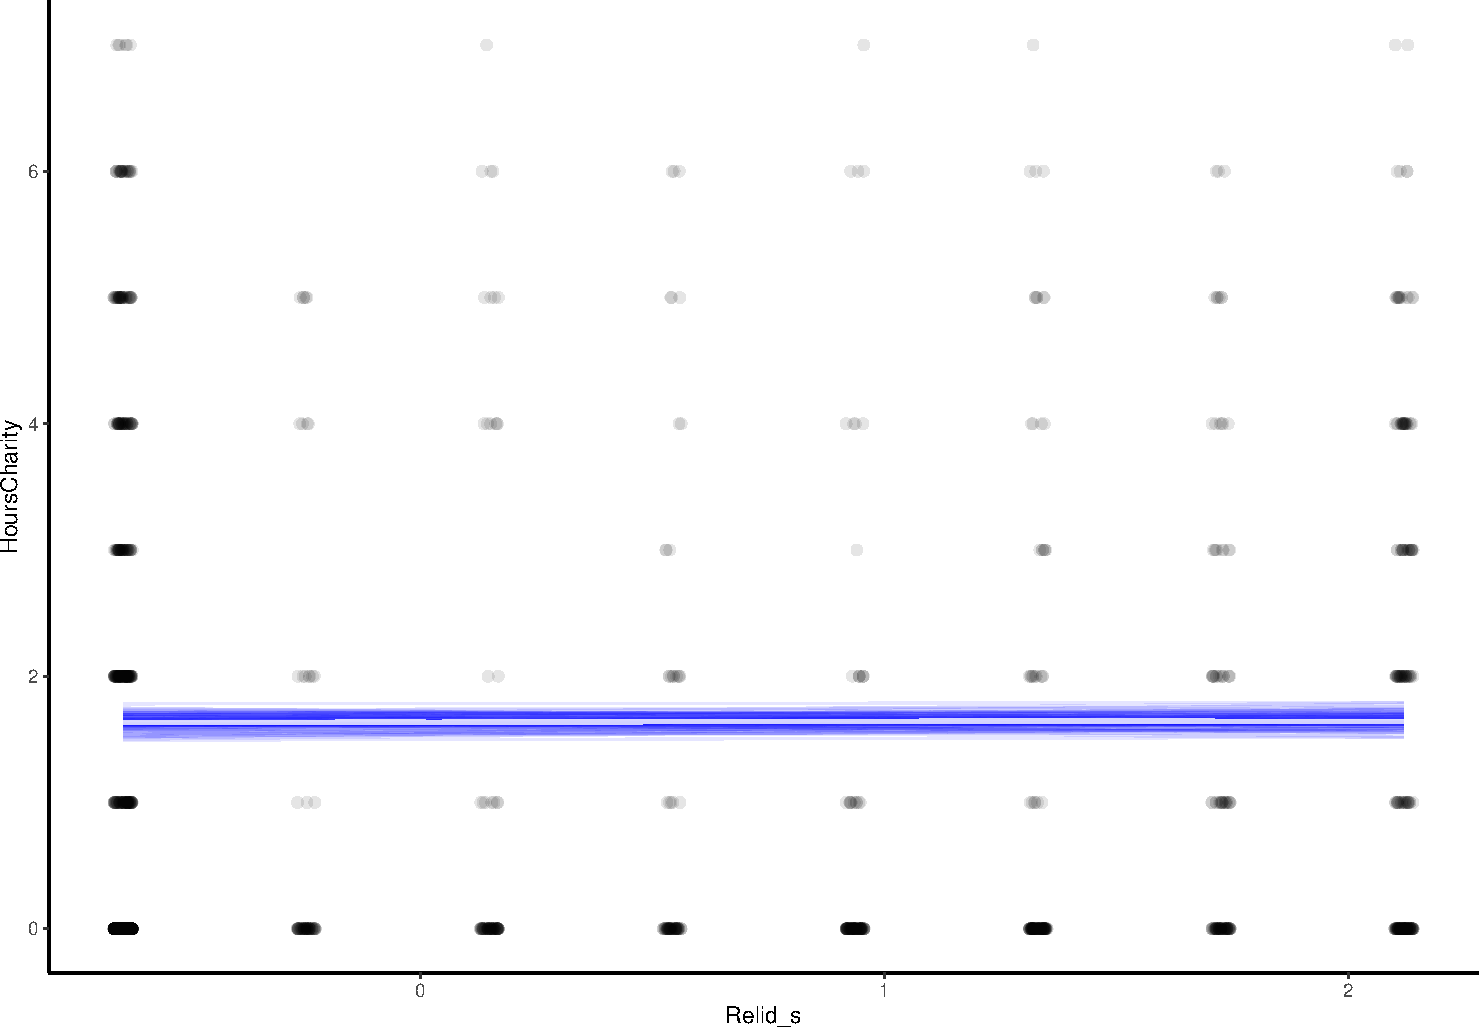
\includegraphics{slides_files/figure-beamer/unnamed-chunk-54-3.pdf}
\end{block}

\begin{block}{Predicted effects of income:}
\protect\hypertarget{predicted-effects-of-income}{}
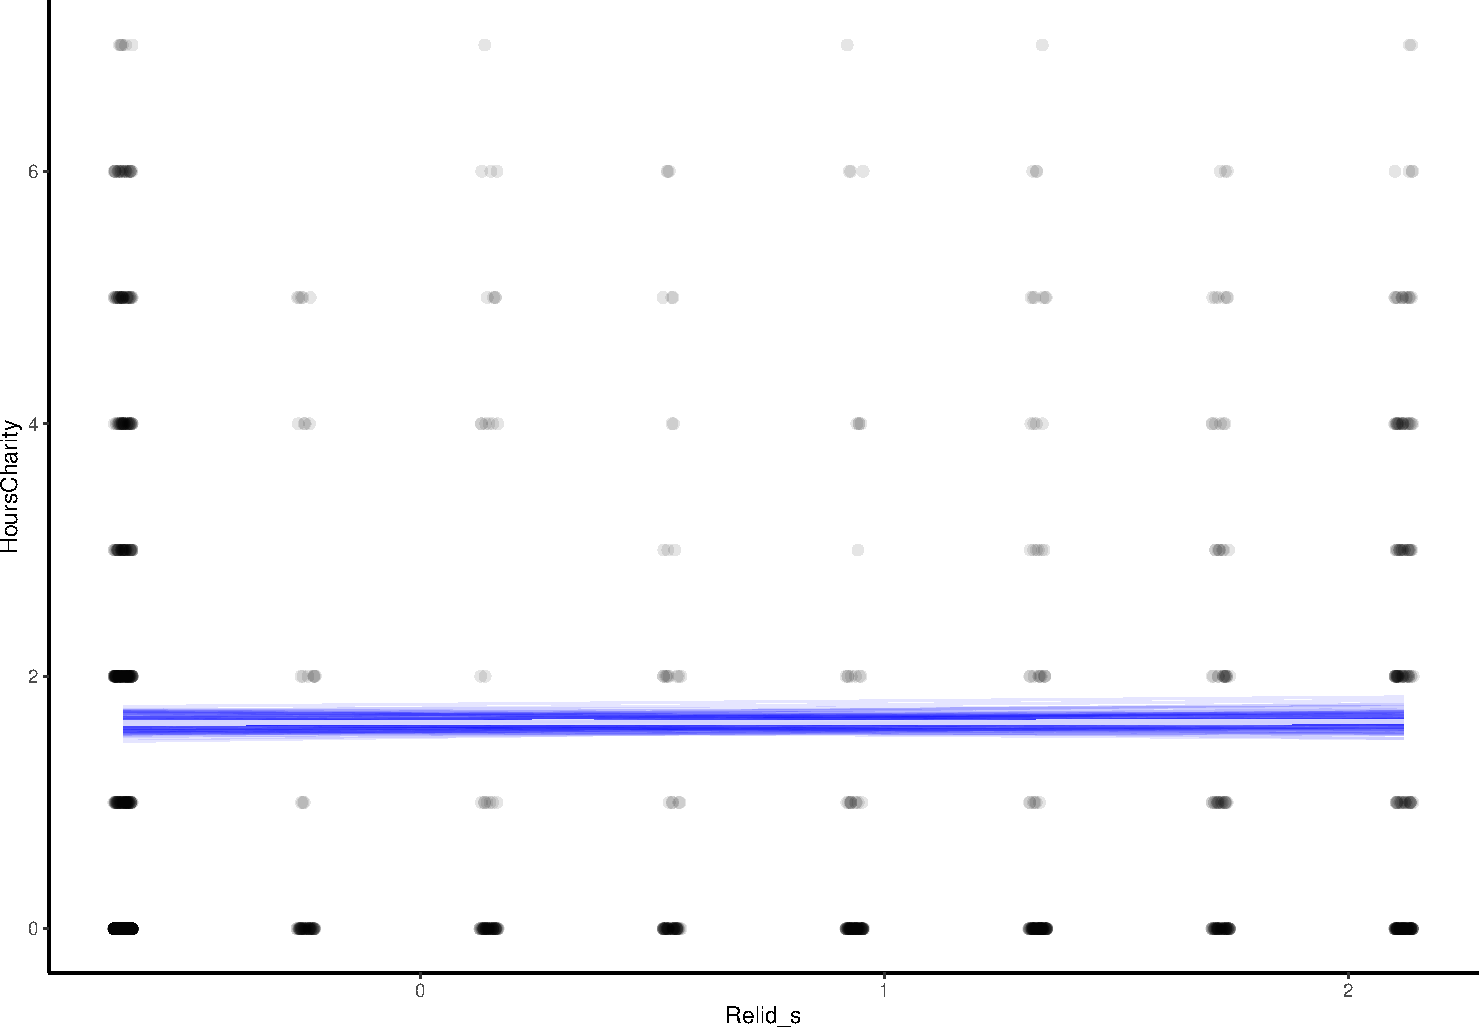
\includegraphics{slides_files/figure-beamer/unnamed-chunk-55-1.pdf}
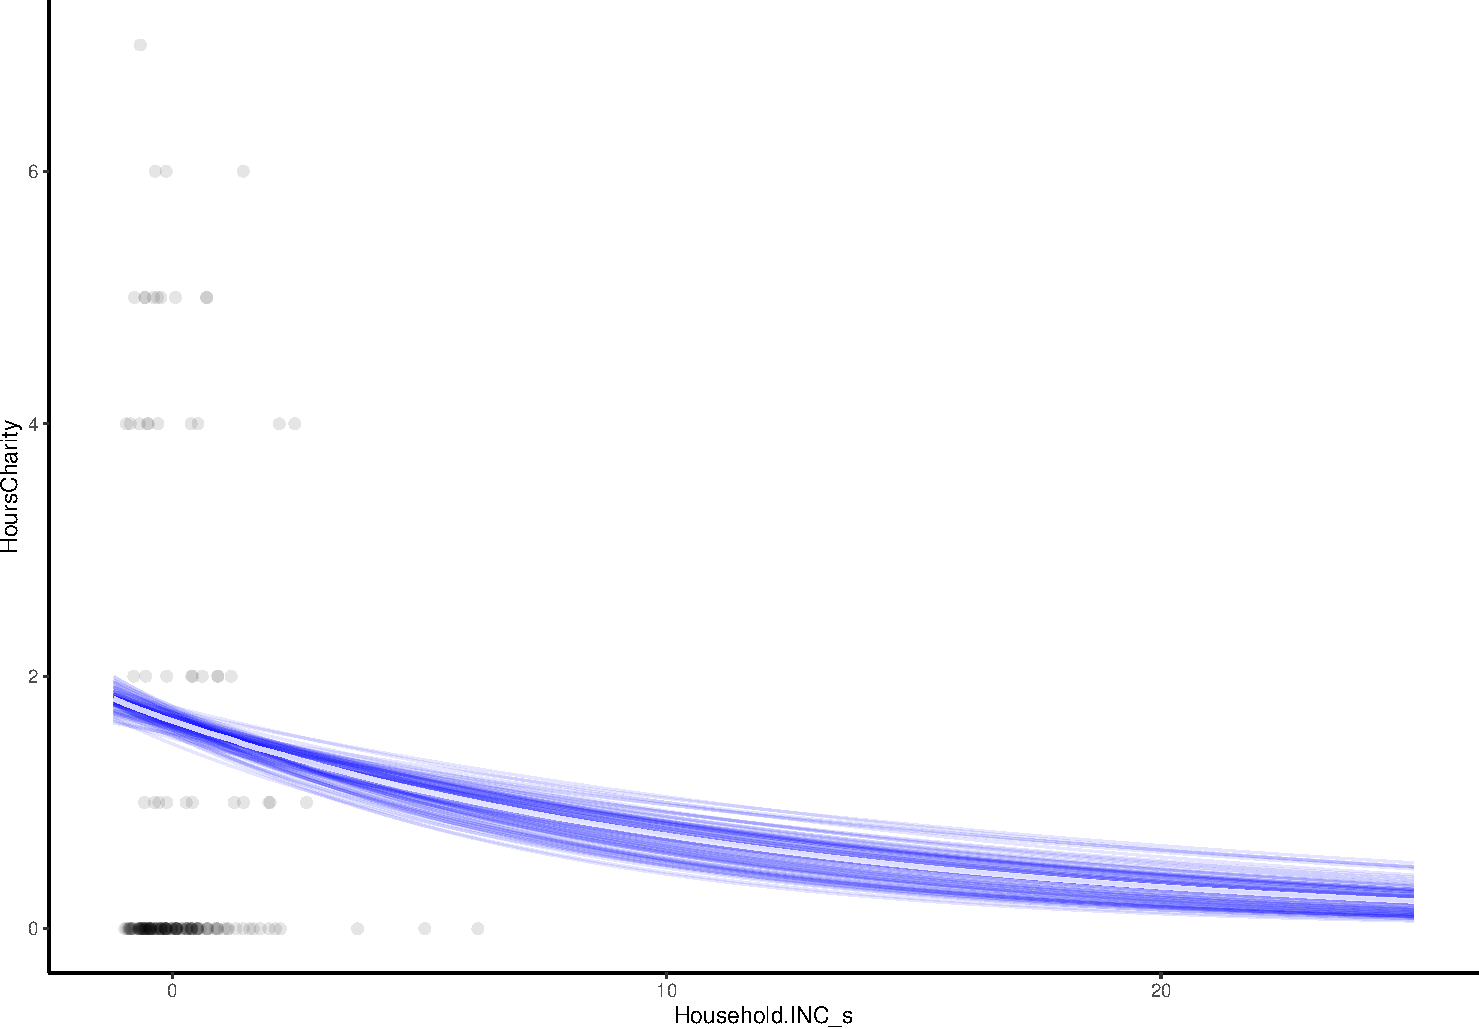
\includegraphics{slides_files/figure-beamer/unnamed-chunk-55-2.pdf}
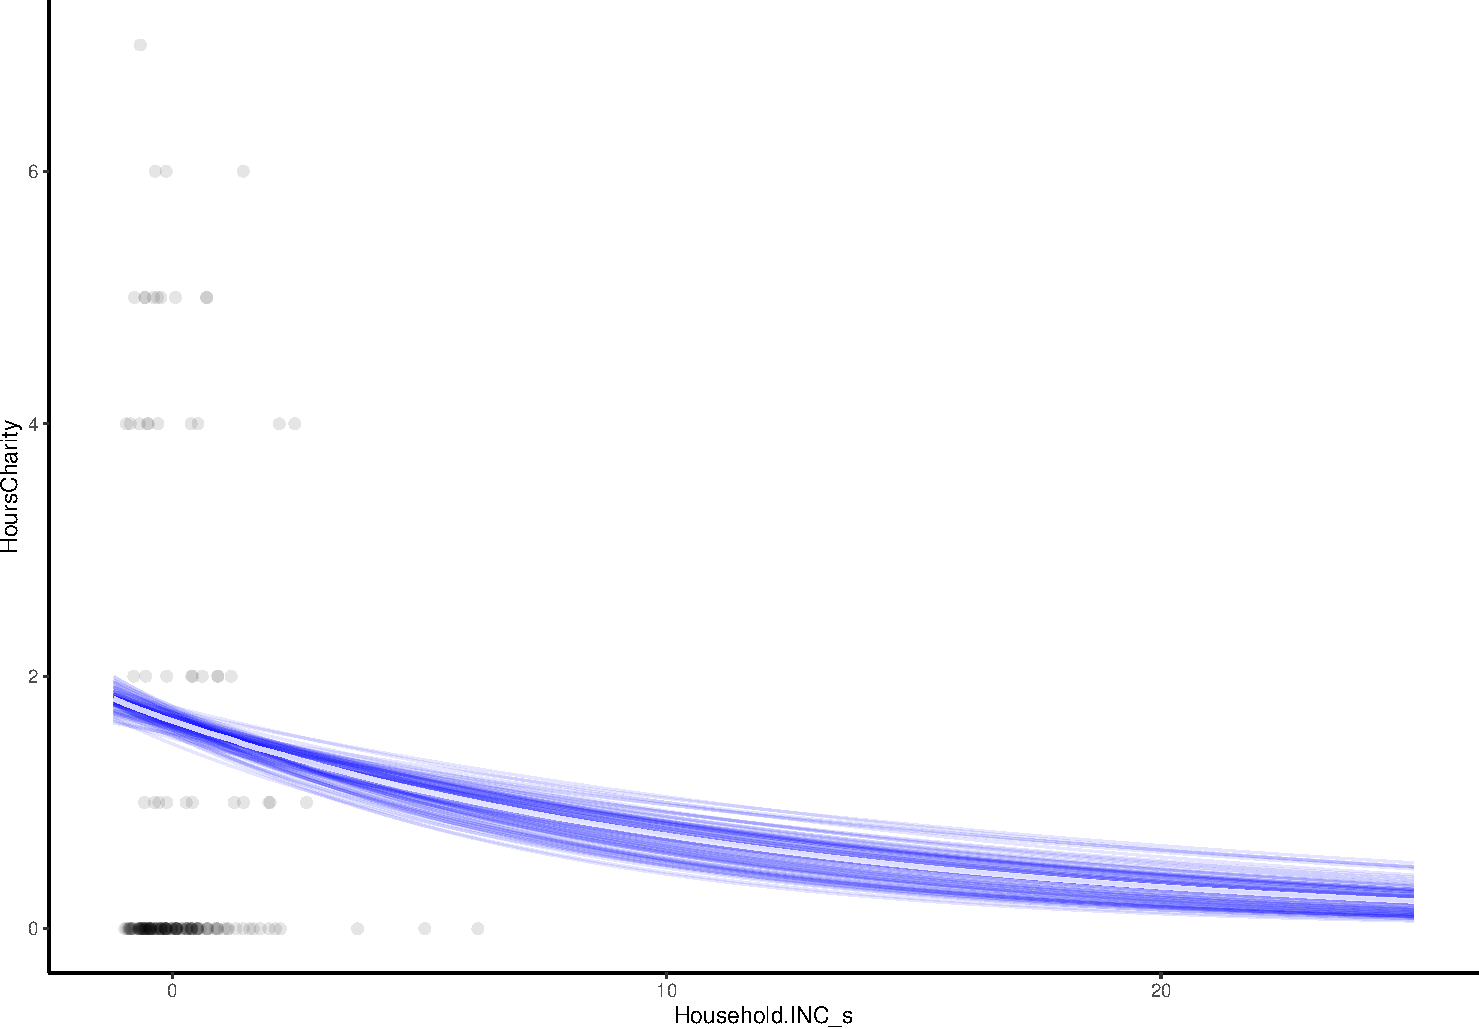
\includegraphics{slides_files/figure-beamer/unnamed-chunk-55-3.pdf}
\end{block}

\begin{block}{Negative binomial zero-inflated model}
\protect\hypertarget{negative-binomial-zero-inflated-model}{}
\end{block}

\begin{block}{Results}
\protect\hypertarget{results-4}{}
\begin{verbatim}
##  Family: zero_inflated_negbinomial 
##   Links: mu = log; shape = identity; zi = identity 
## Formula: HoursCharity ~ Relid_s + Household.INC_s 
##    Data: nz (Number of observations: 2796) 
## Samples: 4 chains, each with iter = 2000; warmup = 1000; thin = 1;
##          total post-warmup samples = 4000
## 
## Population-Level Effects: 
##                 Estimate Est.Error l-95% CI u-95% CI Rhat Bulk_ESS Tail_ESS
## Intercept           0.89      0.17     0.52     1.17 1.00      949      885
## Relid_s             0.21      0.06     0.11     0.33 1.00     1456     1698
## Household.INC_s    -0.07      0.05    -0.16     0.03 1.00     2061     2040
## 
## Family Specific Parameters: 
##       Estimate Est.Error l-95% CI u-95% CI Rhat Bulk_ESS Tail_ESS
## shape     0.28      0.07     0.16     0.42 1.00      938      914
## zi        0.35      0.11     0.07     0.50 1.00      939      697
## 
## Samples were drawn using sampling(NUTS). For each parameter, Bulk_ESS
## and Tail_ESS are effective sample size measures, and Rhat is the potential
## scale reduction factor on split chains (at convergence, Rhat = 1).
\end{verbatim}
\end{block}

\begin{block}{Compare models}
\protect\hypertarget{compare-models}{}
\begin{verbatim}
##    elpd_diff se_diff
## b1     0.0       0.0
## b0 -1514.8     207.5
\end{verbatim}
\end{block}

\begin{block}{Translation}
\protect\hypertarget{translation}{}
We can translate the \texttt{loo\_compare} output into a \texttt{waic}
convention as:

\begin{verbatim}
##    waic_diff       se
## b1     0.000   0.0000
## b0  3029.657 414.9648
\end{verbatim}
\end{block}

\begin{block}{What predicts the zeros?}
\protect\hypertarget{what-predicts-the-zeros}{}
\begin{verbatim}
##  Family: zero_inflated_negbinomial 
##   Links: mu = log; shape = identity; zi = identity 
## Formula: HoursCharity ~ Relid_s + Household.INC_s 
##    Data: nz (Number of observations: 2796) 
## Samples: 4 chains, each with iter = 2000; warmup = 1000; thin = 1;
##          total post-warmup samples = 4000
## 
## Population-Level Effects: 
##                 Estimate Est.Error l-95% CI u-95% CI Rhat Bulk_ESS Tail_ESS
## Intercept           0.89      0.17     0.52     1.17 1.00      949      885
## Relid_s             0.21      0.06     0.11     0.33 1.00     1456     1698
## Household.INC_s    -0.07      0.05    -0.16     0.03 1.00     2061     2040
## 
## Family Specific Parameters: 
##       Estimate Est.Error l-95% CI u-95% CI Rhat Bulk_ESS Tail_ESS
## shape     0.28      0.07     0.16     0.42 1.00      938      914
## zi        0.35      0.11     0.07     0.50 1.00      939      697
## 
## Samples were drawn using sampling(NUTS). For each parameter, Bulk_ESS
## and Tail_ESS are effective sample size measures, and Rhat is the potential
## scale reduction factor on split chains (at convergence, Rhat = 1).
\end{verbatim}
\end{block}

\begin{block}{Intepretation}
\protect\hypertarget{intepretation}{}
The probability of non-volunteering in the preferred model for people
who are at the mean Religious Identification and mean Household income
in this population is \texttt{plogis(.35)} or 0.5866176. More often than
not, we should predict zeros in this population. What predicts the zero
component of the model? We can use this syntax:
\end{block}

\begin{block}{ZI\_NEGBIN Syntax}
\protect\hypertarget{zi_negbin-syntax}{}
\end{block}

\begin{block}{Results}
\protect\hypertarget{results-5}{}
~

HoursCharity

Predictors

Incidence Rate Ratios

CI (95\%)

Count Model

Intercept

3.40

2.85~--~3.95

Relid\_s

1.02

0.94~--~1.11

Household.INC\_s

0.93

0.84~--~1.03

Zero-Inflated Model

Intercept

1.06

0.72~--~1.38

Relid\_s

0.52

0.42~--~0.61

Household.INC\_s

1.02

0.87~--~1.17

Observations

2796

R2 Bayes

0.015
\end{block}

\begin{block}{Interpretation: relid}
\protect\hypertarget{interpretation-relid}{}
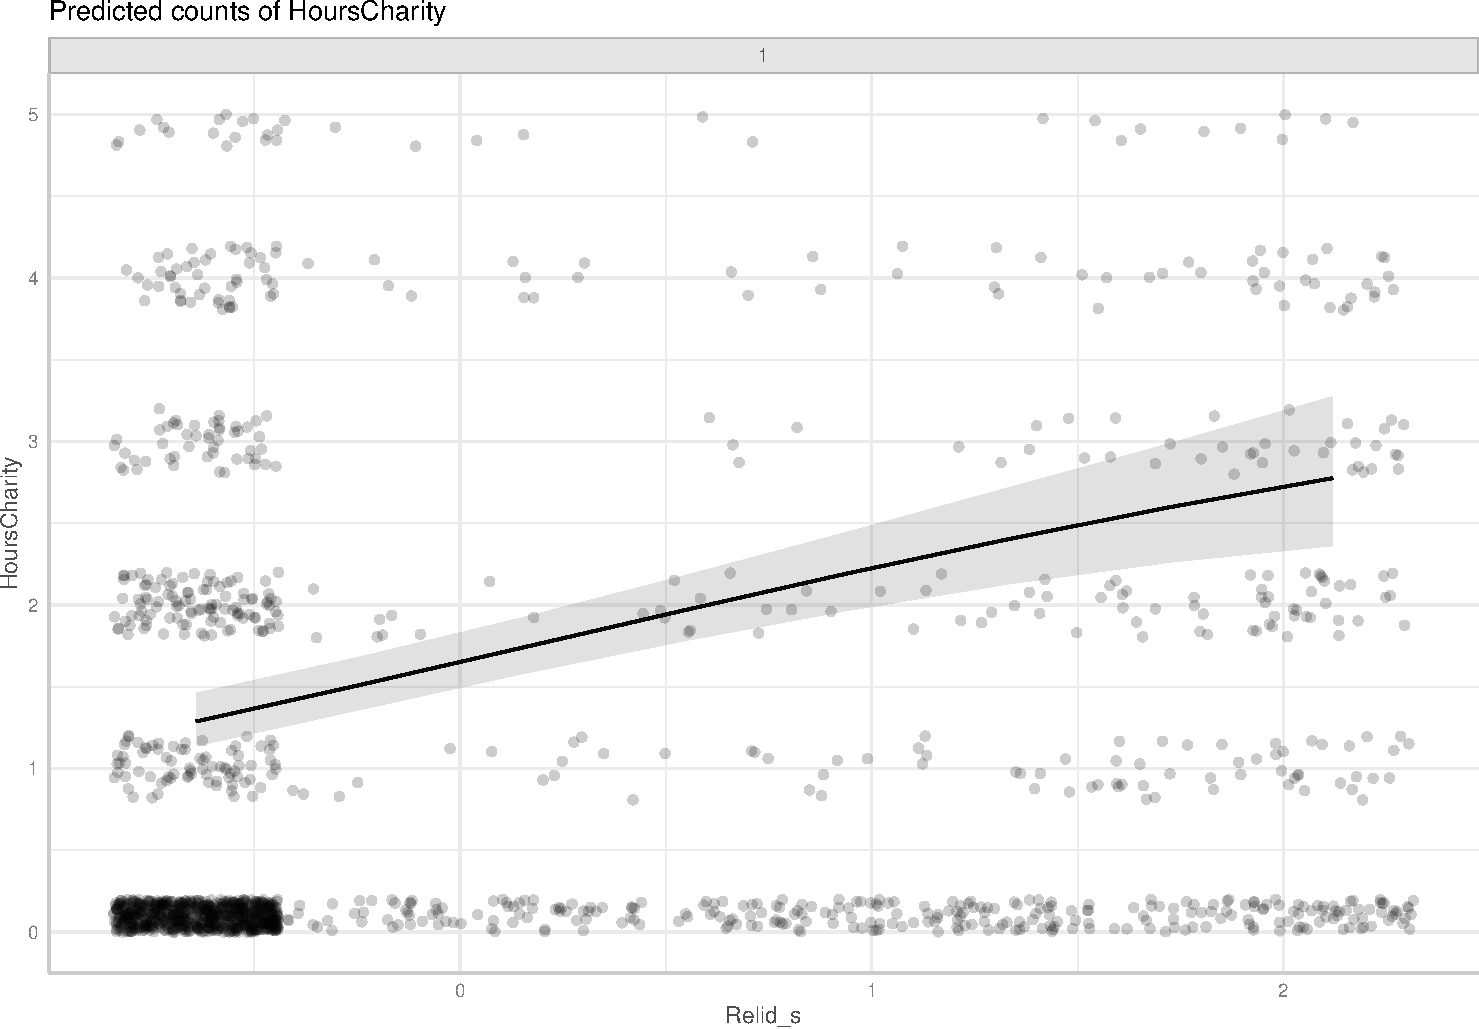
\includegraphics{slides_files/figure-beamer/unnamed-chunk-63-1.pdf}
\end{block}

\begin{block}{Interpretation: Household income}
\protect\hypertarget{interpretation-household-income}{}
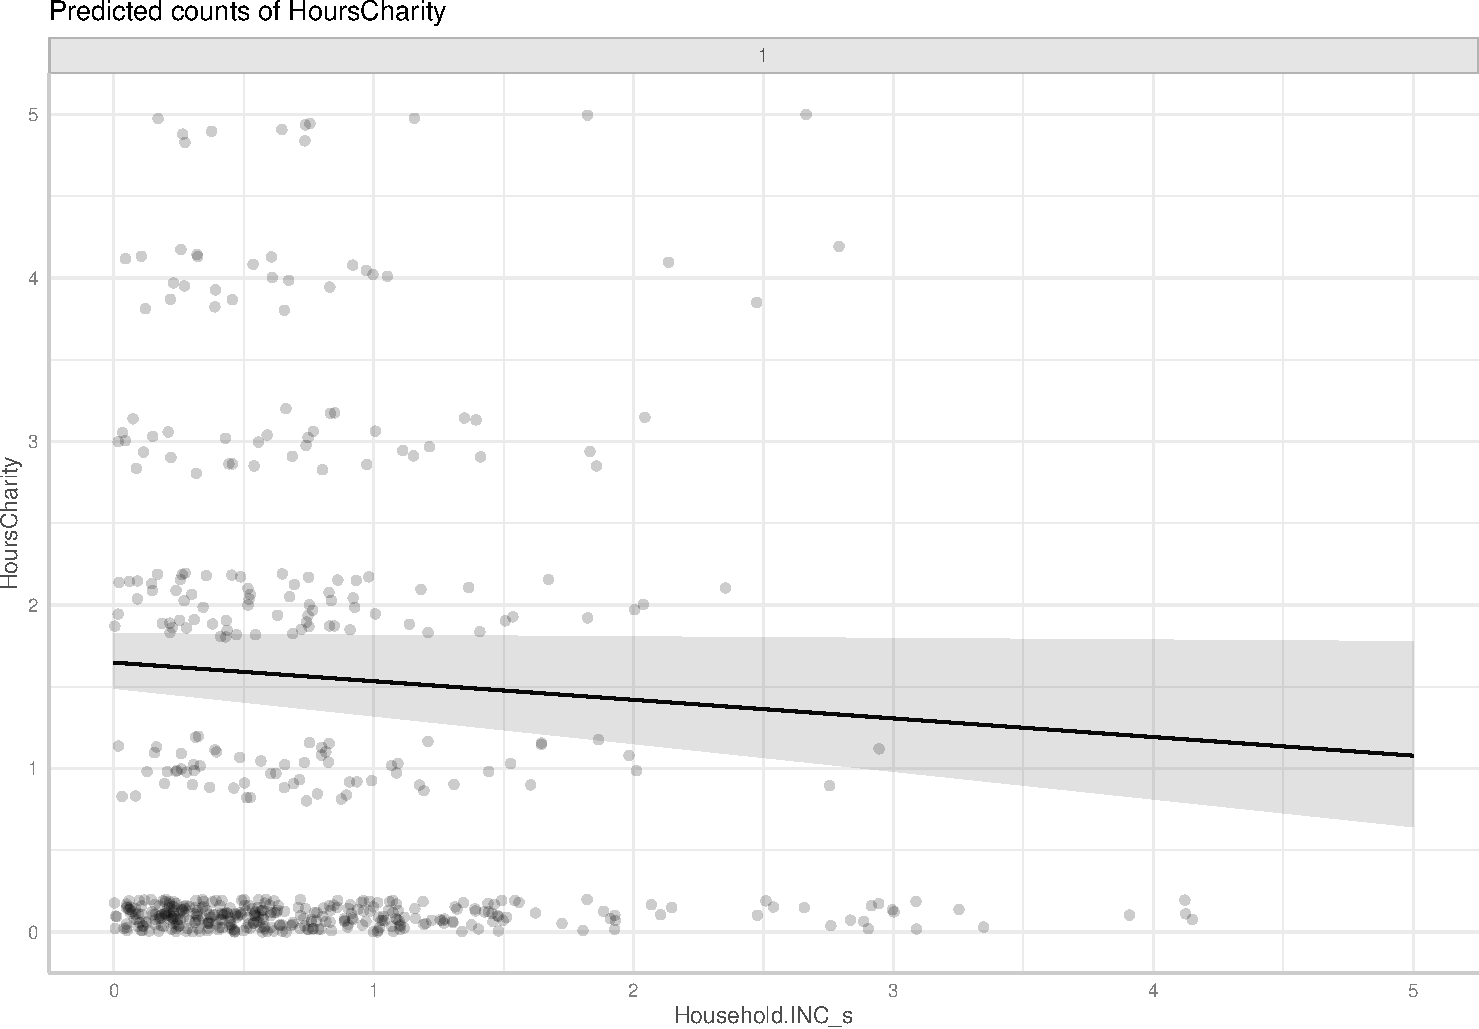
\includegraphics{slides_files/figure-beamer/unnamed-chunk-64-1.pdf}
\end{block}

\begin{block}{Better graphs}
\protect\hypertarget{better-graphs}{}
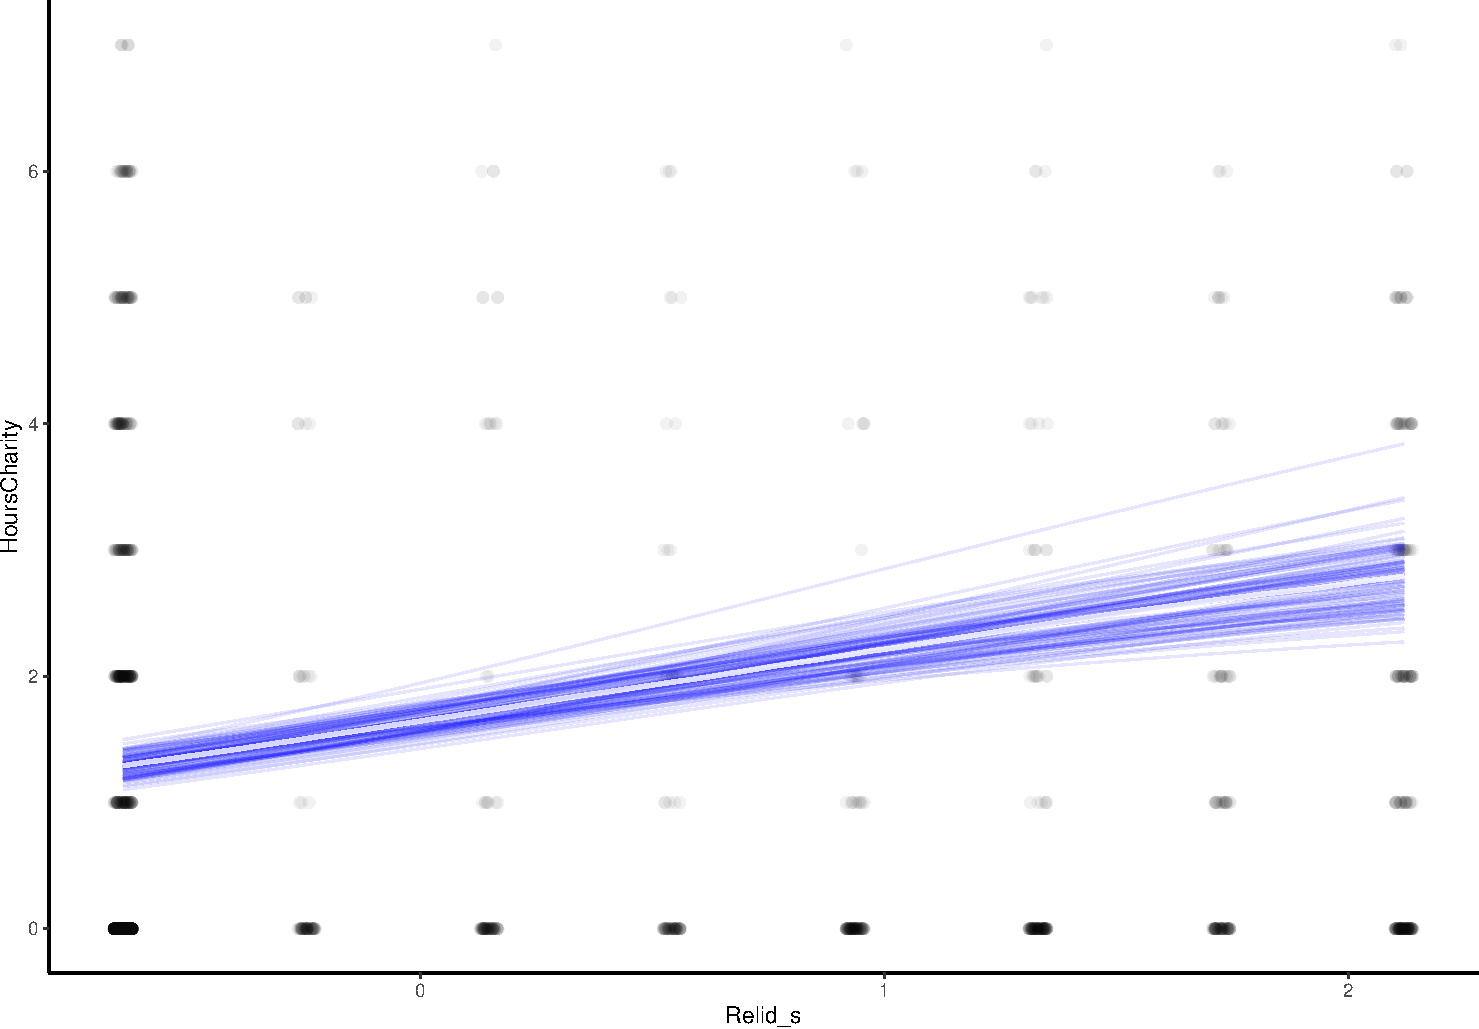
\includegraphics{slides_files/figure-beamer/unnamed-chunk-65-1.pdf}
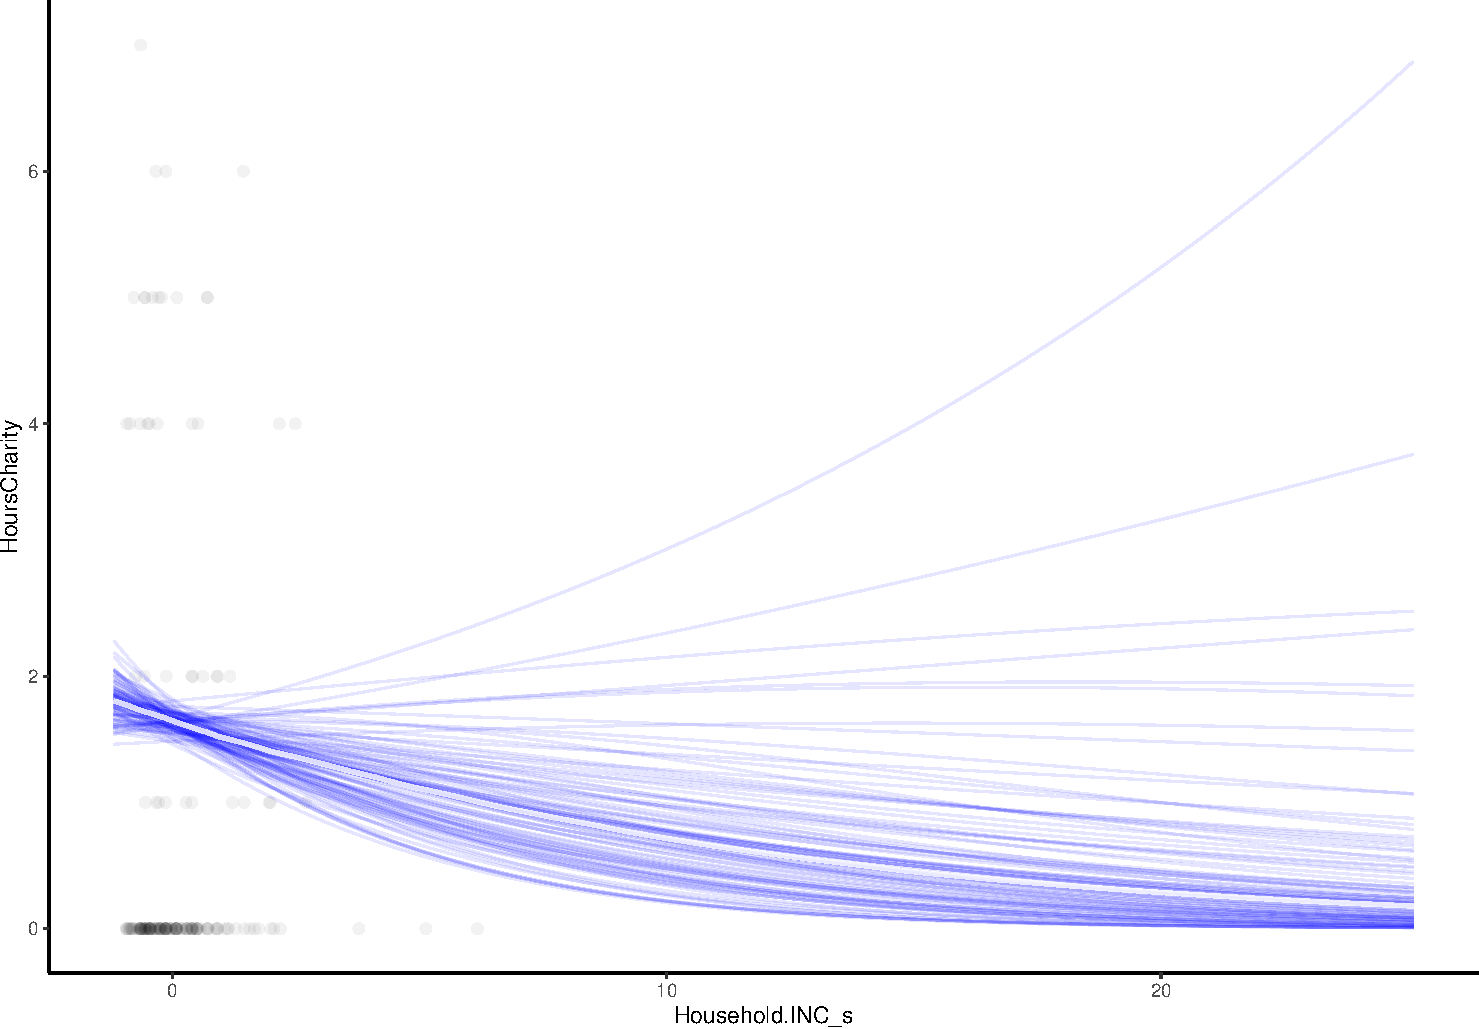
\includegraphics{slides_files/figure-beamer/unnamed-chunk-65-2.pdf}

\begin{verbatim}
## NULL
\end{verbatim}
\end{block}

\begin{block}{Model selection}
\protect\hypertarget{model-selection-1}{}
\begin{verbatim}
##    elpd_diff se_diff
## b2     0.0       0.0
## b1   -50.0      10.1
## b0 -1564.8     206.1
\end{verbatim}
\end{block}

\begin{block}{Model Selection}
\protect\hypertarget{model-selection-2}{}
\begin{verbatim}
##    waic_diff        se
## b2    0.0000   0.00000
## b1  100.0416  20.14189
## b0 3129.6983 412.13260
\end{verbatim}
\end{block}

\begin{block}{Posterior predictive checks:poisson}
\protect\hypertarget{posterior-predictive-checkspoisson}{}
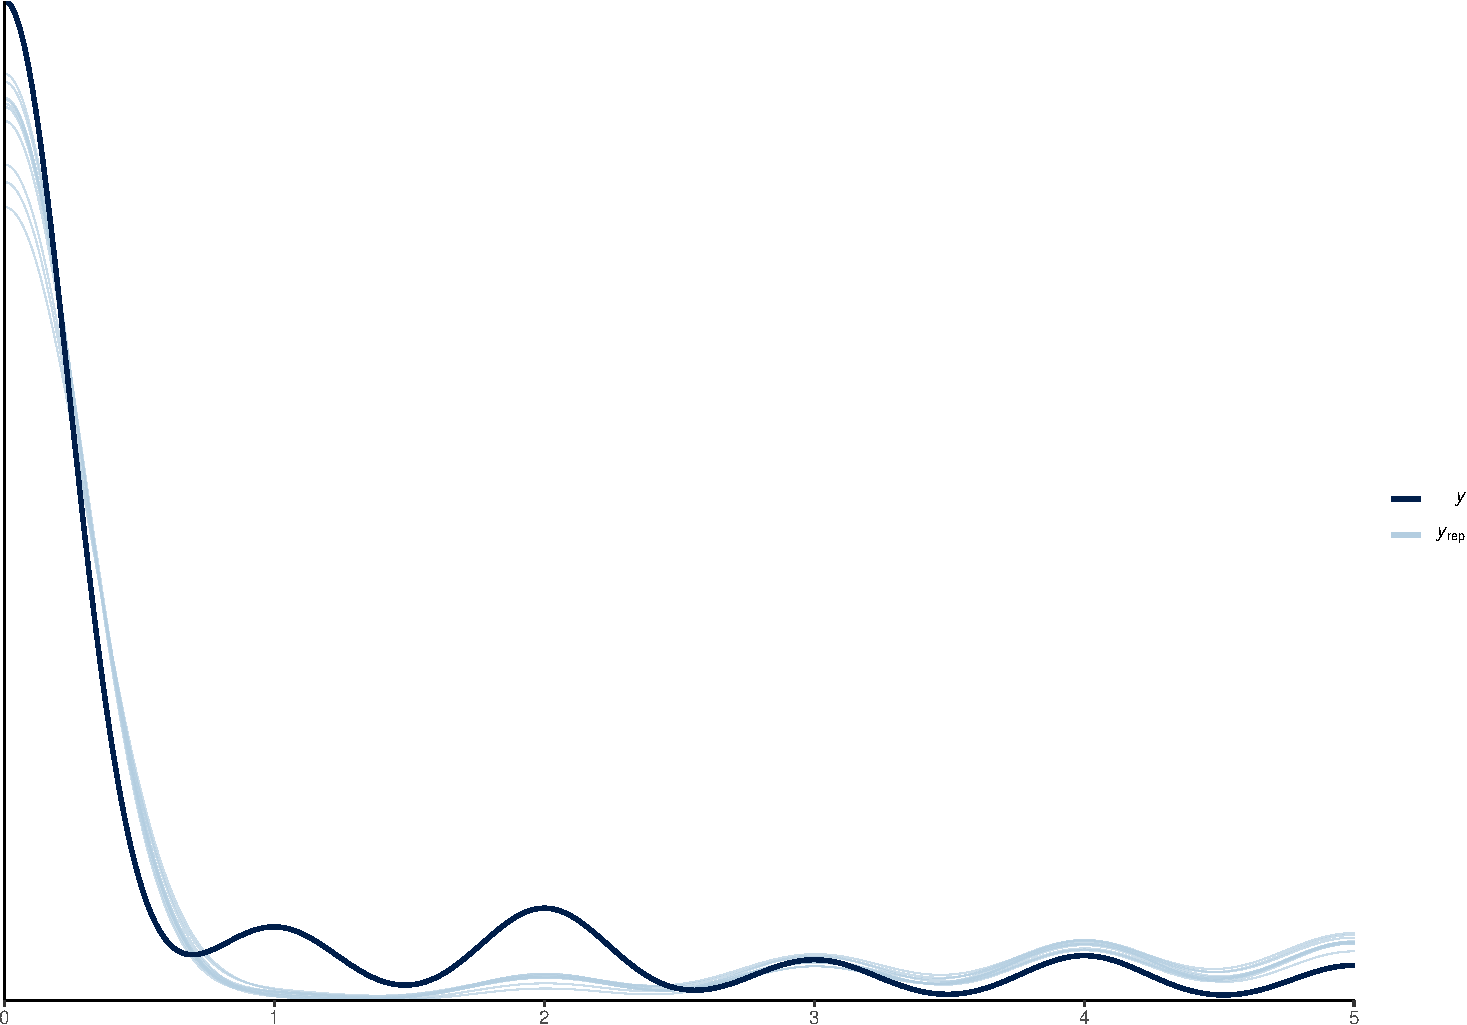
\includegraphics{slides_files/figure-beamer/unnamed-chunk-68-1.pdf}

Zero-inflated negative binomial with no predictors for the
zero-inflation part.
\end{block}

\begin{block}{Posterior predictive checks:zipoisson zinegbin}
\protect\hypertarget{posterior-predictive-checkszipoisson-zinegbin}{}
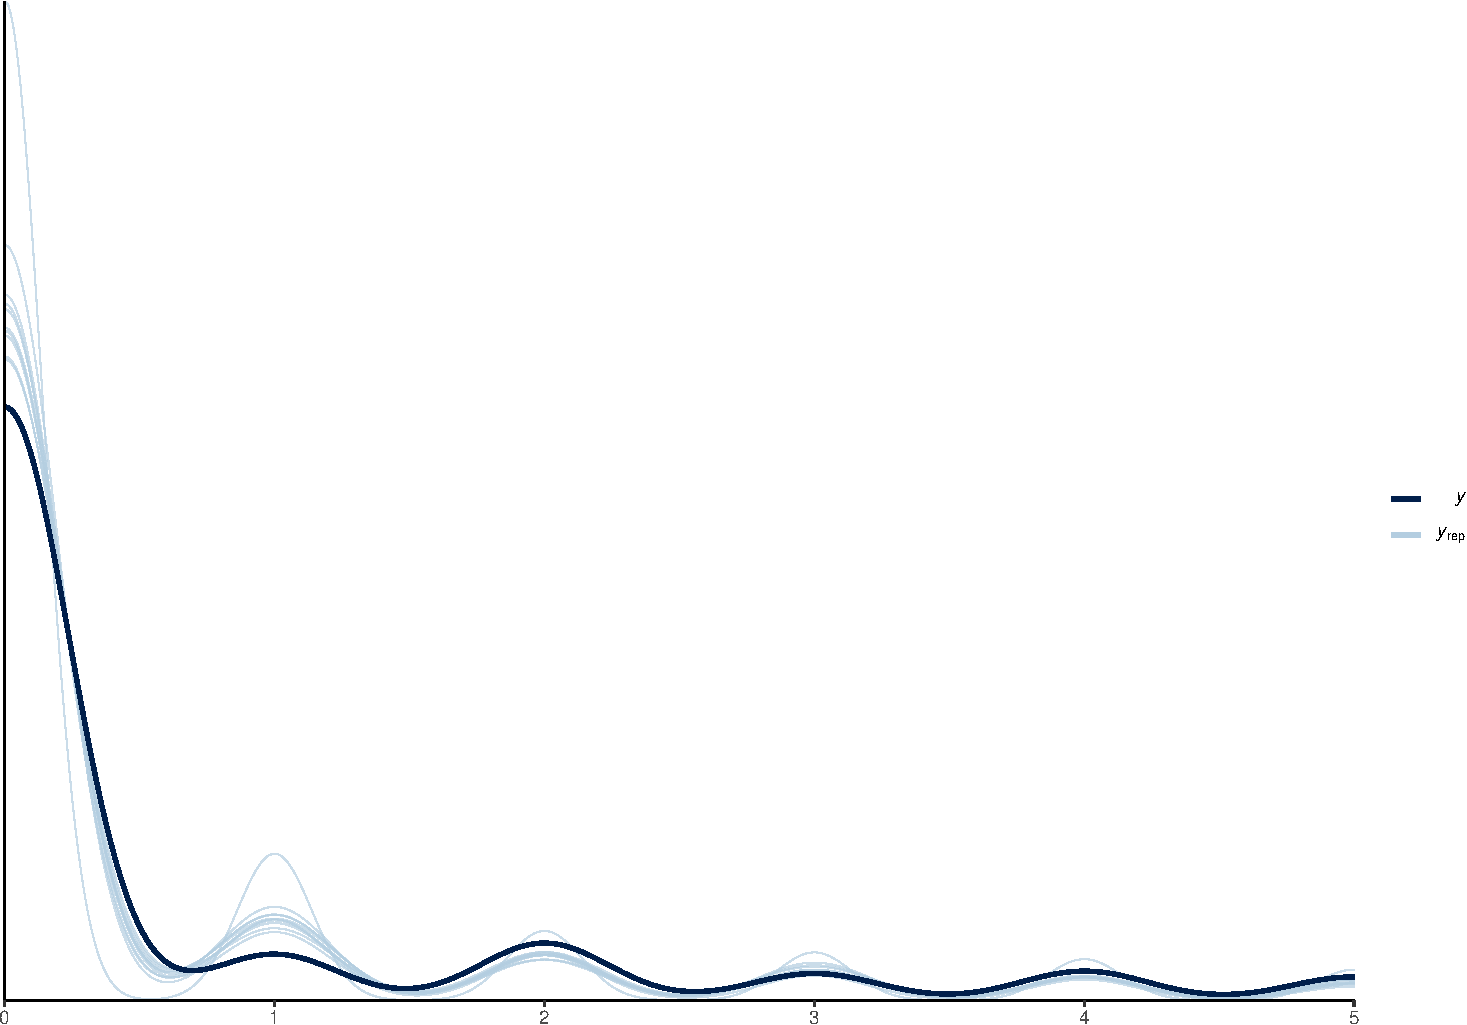
\includegraphics{slides_files/figure-beamer/unnamed-chunk-69-1.pdf}
\end{block}

\begin{block}{Posterior predictive checks: zinegbin}
\protect\hypertarget{posterior-predictive-checks-zinegbin}{}
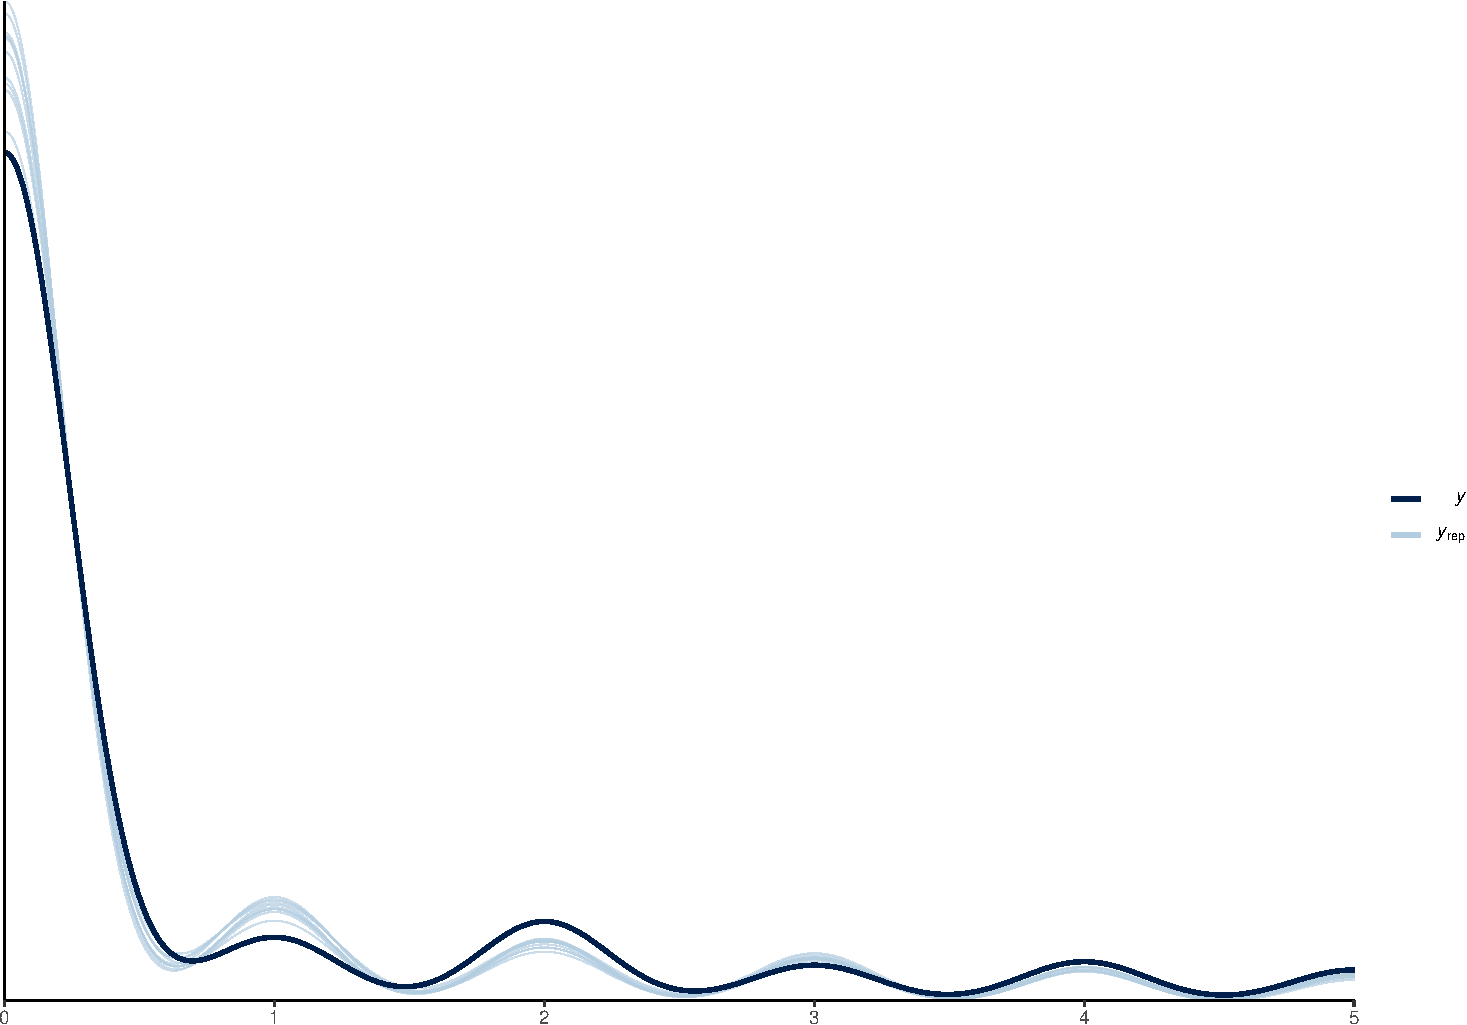
\includegraphics{slides_files/figure-beamer/unnamed-chunk-70-1.pdf}
\end{block}

\begin{block}{Appendix 1}
\protect\hypertarget{appendix-1}{}
If you want to graph each predictor separately emply the
\texttt{{[}{[}1{]}{]}} or \texttt{{[}{[}2{]}} syntax as follows:{]}

Predicted effects of religious identification
\end{block}

\begin{block}{Aside}
\protect\hypertarget{aside}{}
\end{block}

\begin{block}{Plot}
\protect\hypertarget{plot}{}
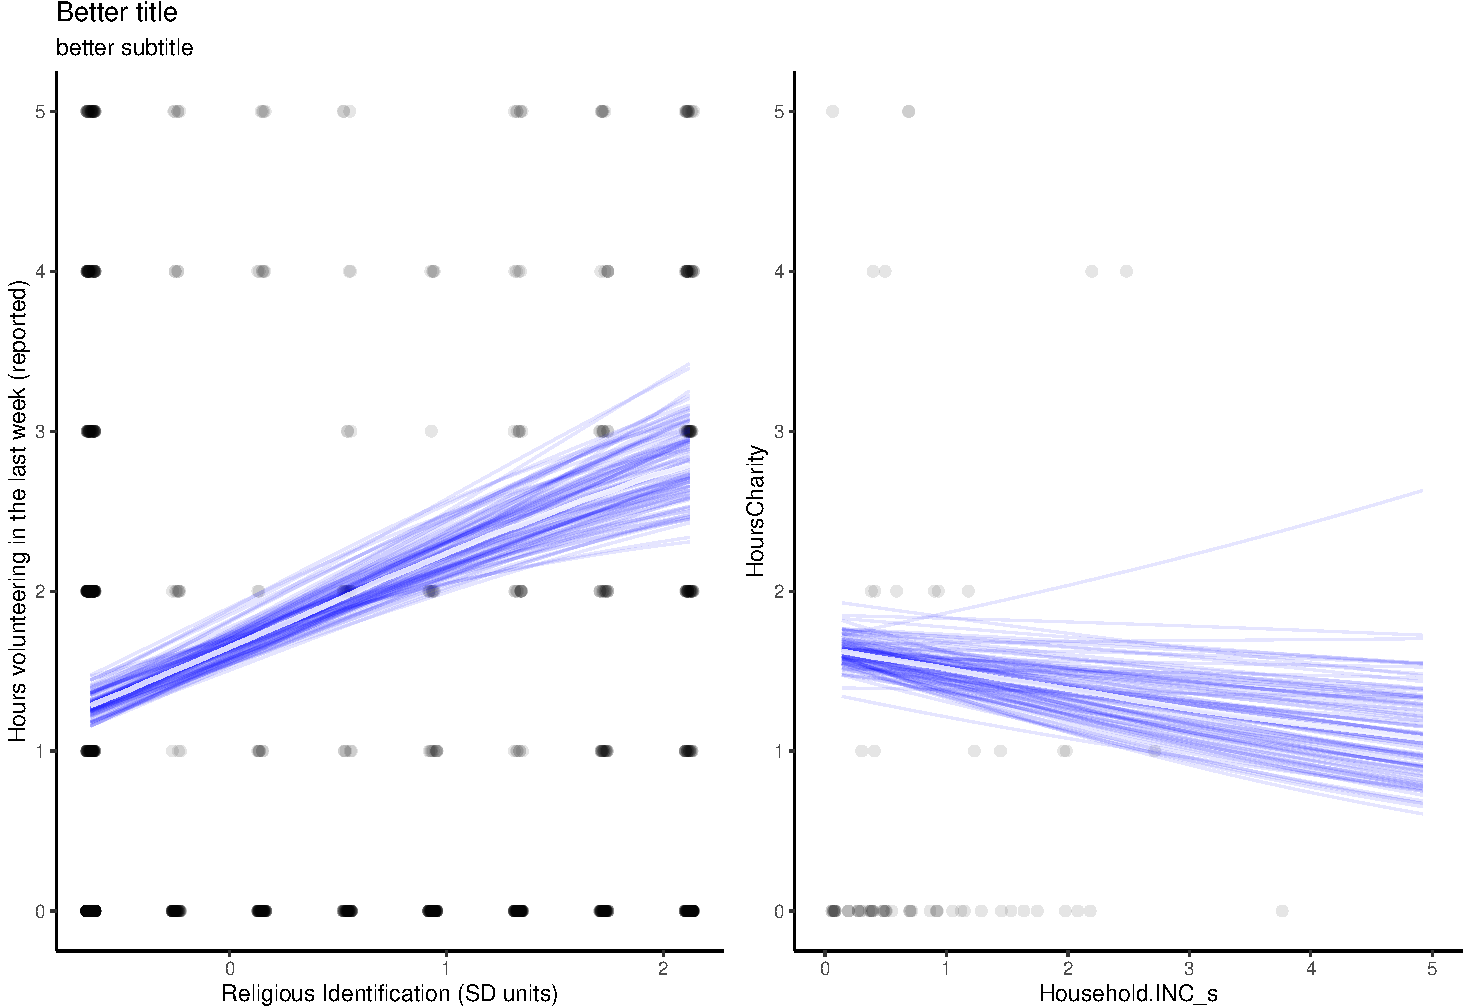
\includegraphics{slides_files/figure-beamer/unnamed-chunk-74-1.pdf}
\end{block}

\begin{block}{Acknowledgments and References}
\protect\hypertarget{acknowledgments-and-references}{}
Gelman, Hill, and Vehtari (2020)

Kurz (2020)

Bürkner and Vuorre (2019)
\end{block}

\begin{block}{Bibliography}
\protect\hypertarget{bibliography}{}
\hypertarget{refs}{}
\begin{CSLReferences}{1}{0}
\leavevmode\hypertarget{ref-buxfcrkner2019}{}%
Bürkner, Paul-Christian, and Matti Vuorre. 2019. {``Ordinal Regression
Models in Psychology: A Tutorial.''} \emph{Advances in Methods and
Practices in Psychological Science} 2 (1): 77--101.

\leavevmode\hypertarget{ref-gelman2020}{}%
Gelman, Andrew, Jennifer Hill, and Aki Vehtari. 2020. \emph{Regression
and Other Stories}. Cambridge University Press.

\leavevmode\hypertarget{ref-kurz2020}{}%
Kurz, A. Solomon. 2020. Zenodo.
\url{https://doi.org/10.5281/zenodo.4080013}.

\end{CSLReferences}
\end{block}
\end{frame}

\end{document}
